In this section, we present user interfaces for Students and Educators. We created a detailed user interface design to inform the reader from a broader perspective.  It provides a clear understanding of how the end-user will interact with the software. This visual representation can demonstrate the flow and layout of the application, making it easier for stakeholders to grasp the user experience. In the UI design we aim to serve as a common language for all stakeholders, including developers, designers, project managers, and clients. It helps in bridging the gap between non-technical and technical team members with help of graphical demonstration. We tried to create every screen possible in order to inform to developers and stakeholders as much as possible. Developer can simplify and advance this user interface designs if they needed.
\\
Naturally runtime views contain much information however user design shows the application from students and educators. However, every mockup is somehow related to a runtime view. Related runtime views are shown.

\begin{center}
    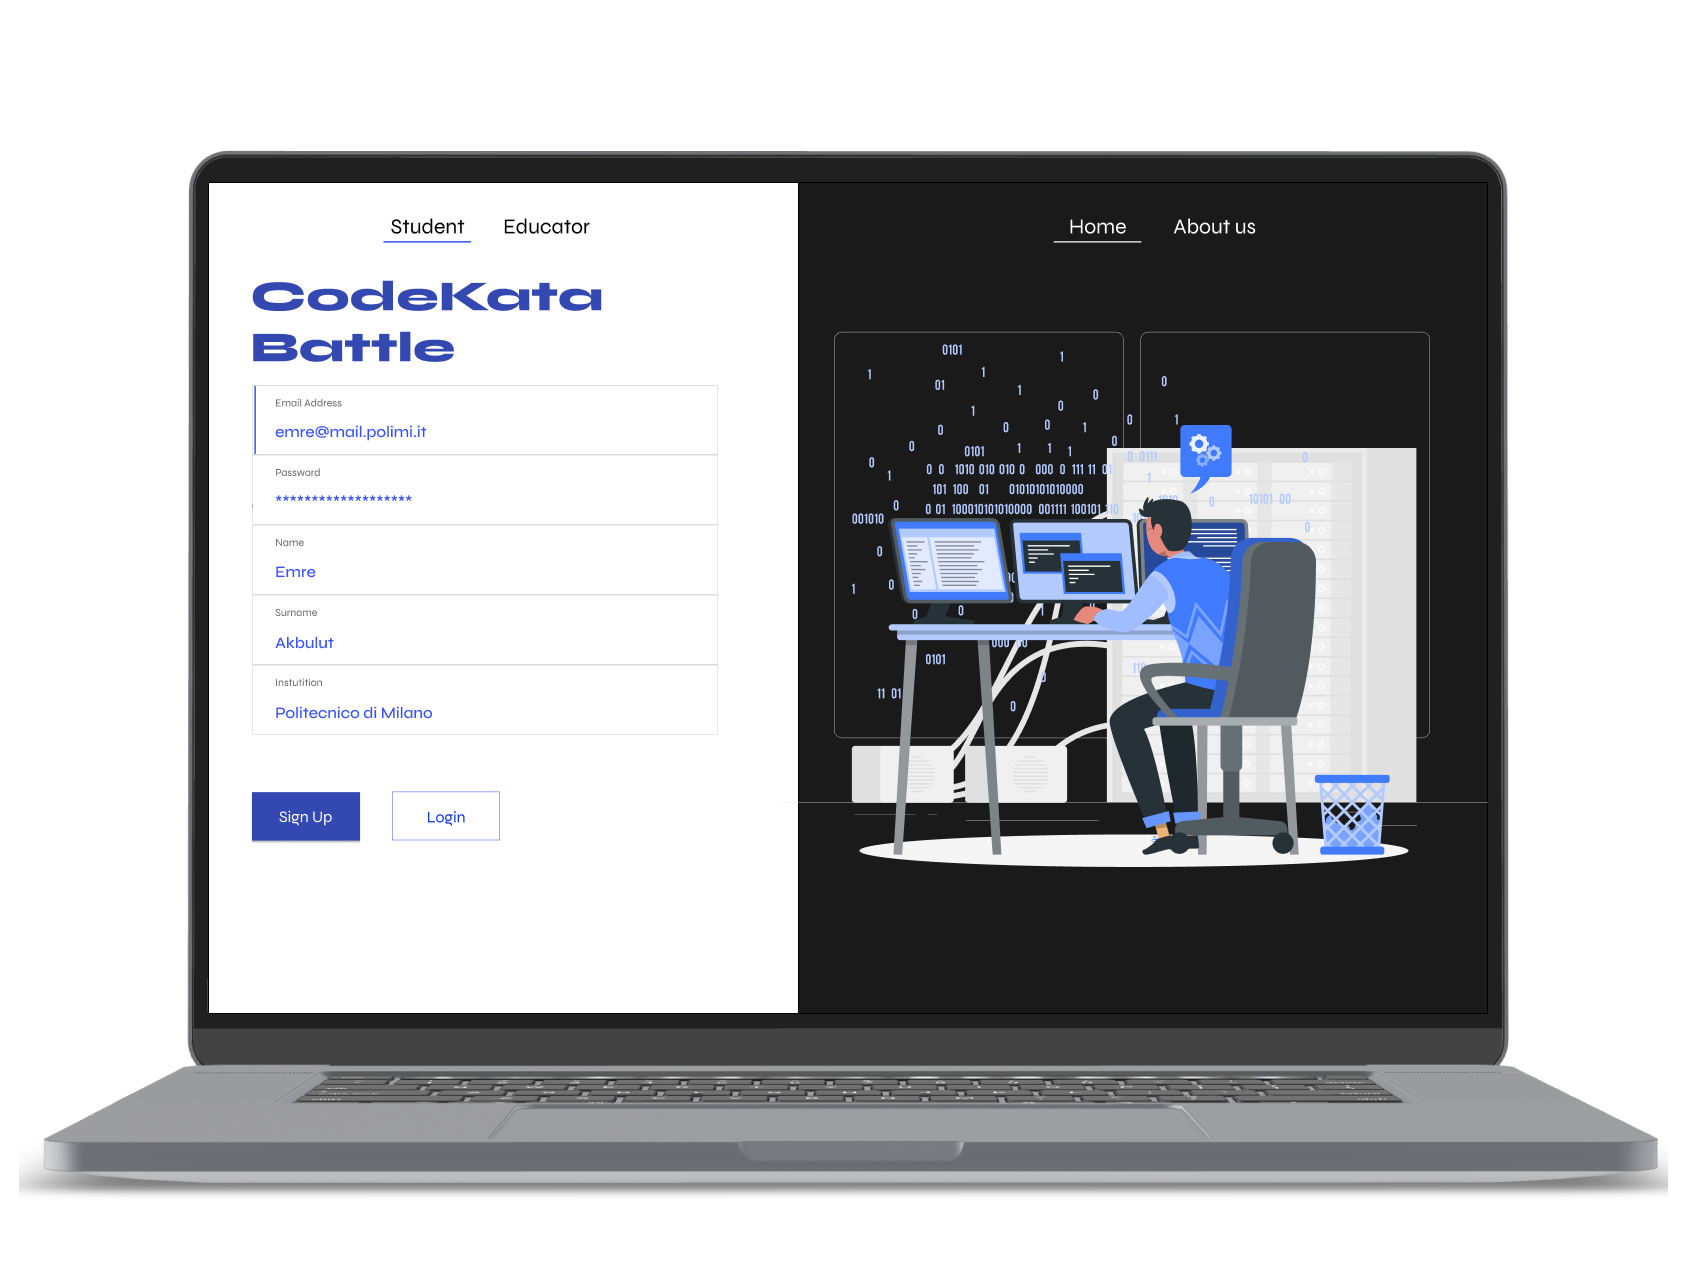
\includegraphics[scale=0.13]{Images/ui-ux/student_signup.png}
    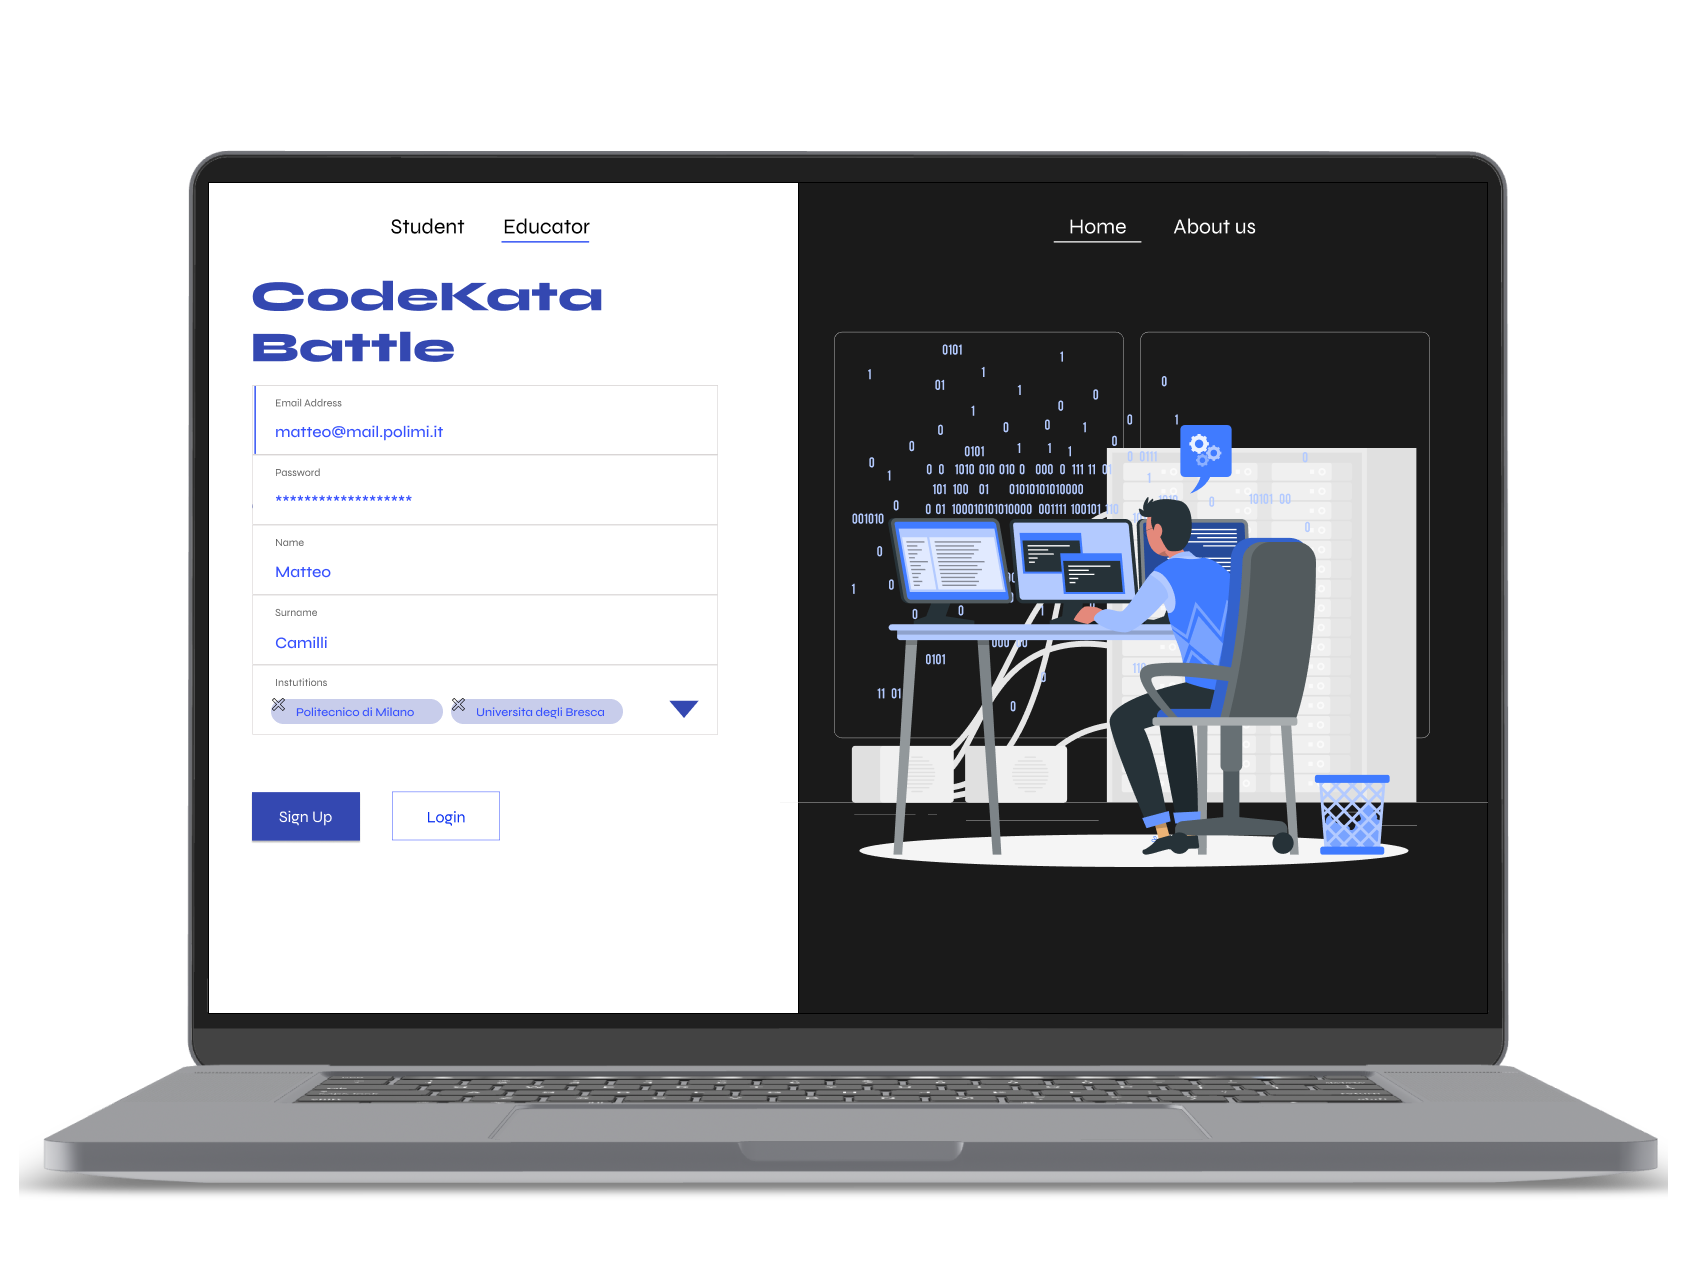
\includegraphics[scale=0.13]{Images/ui-ux/educator_signup.png}
    (a) $UI_{1}$ Sign up Screens 
\end{center}

\begin{center}
    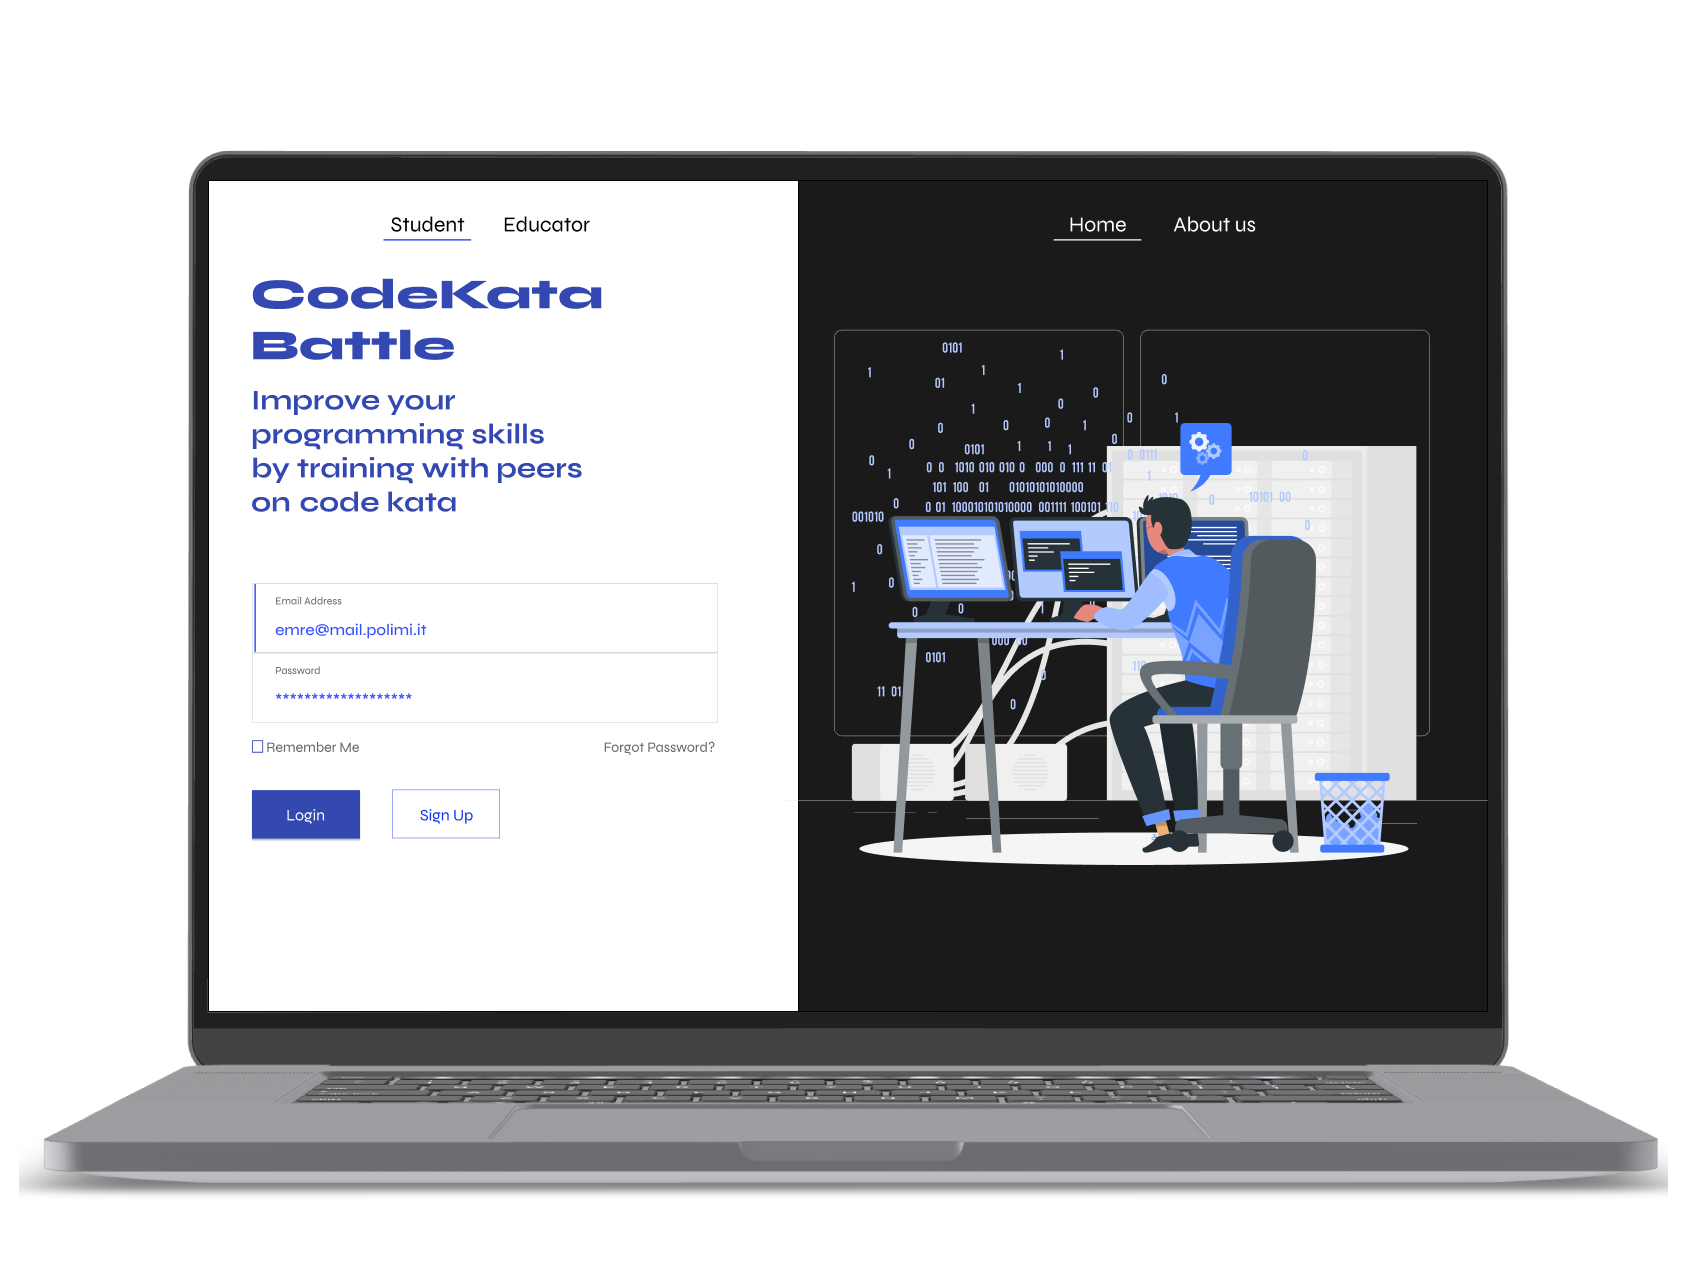
\includegraphics[scale=0.13]{Images/ui-ux/student_login.png}
    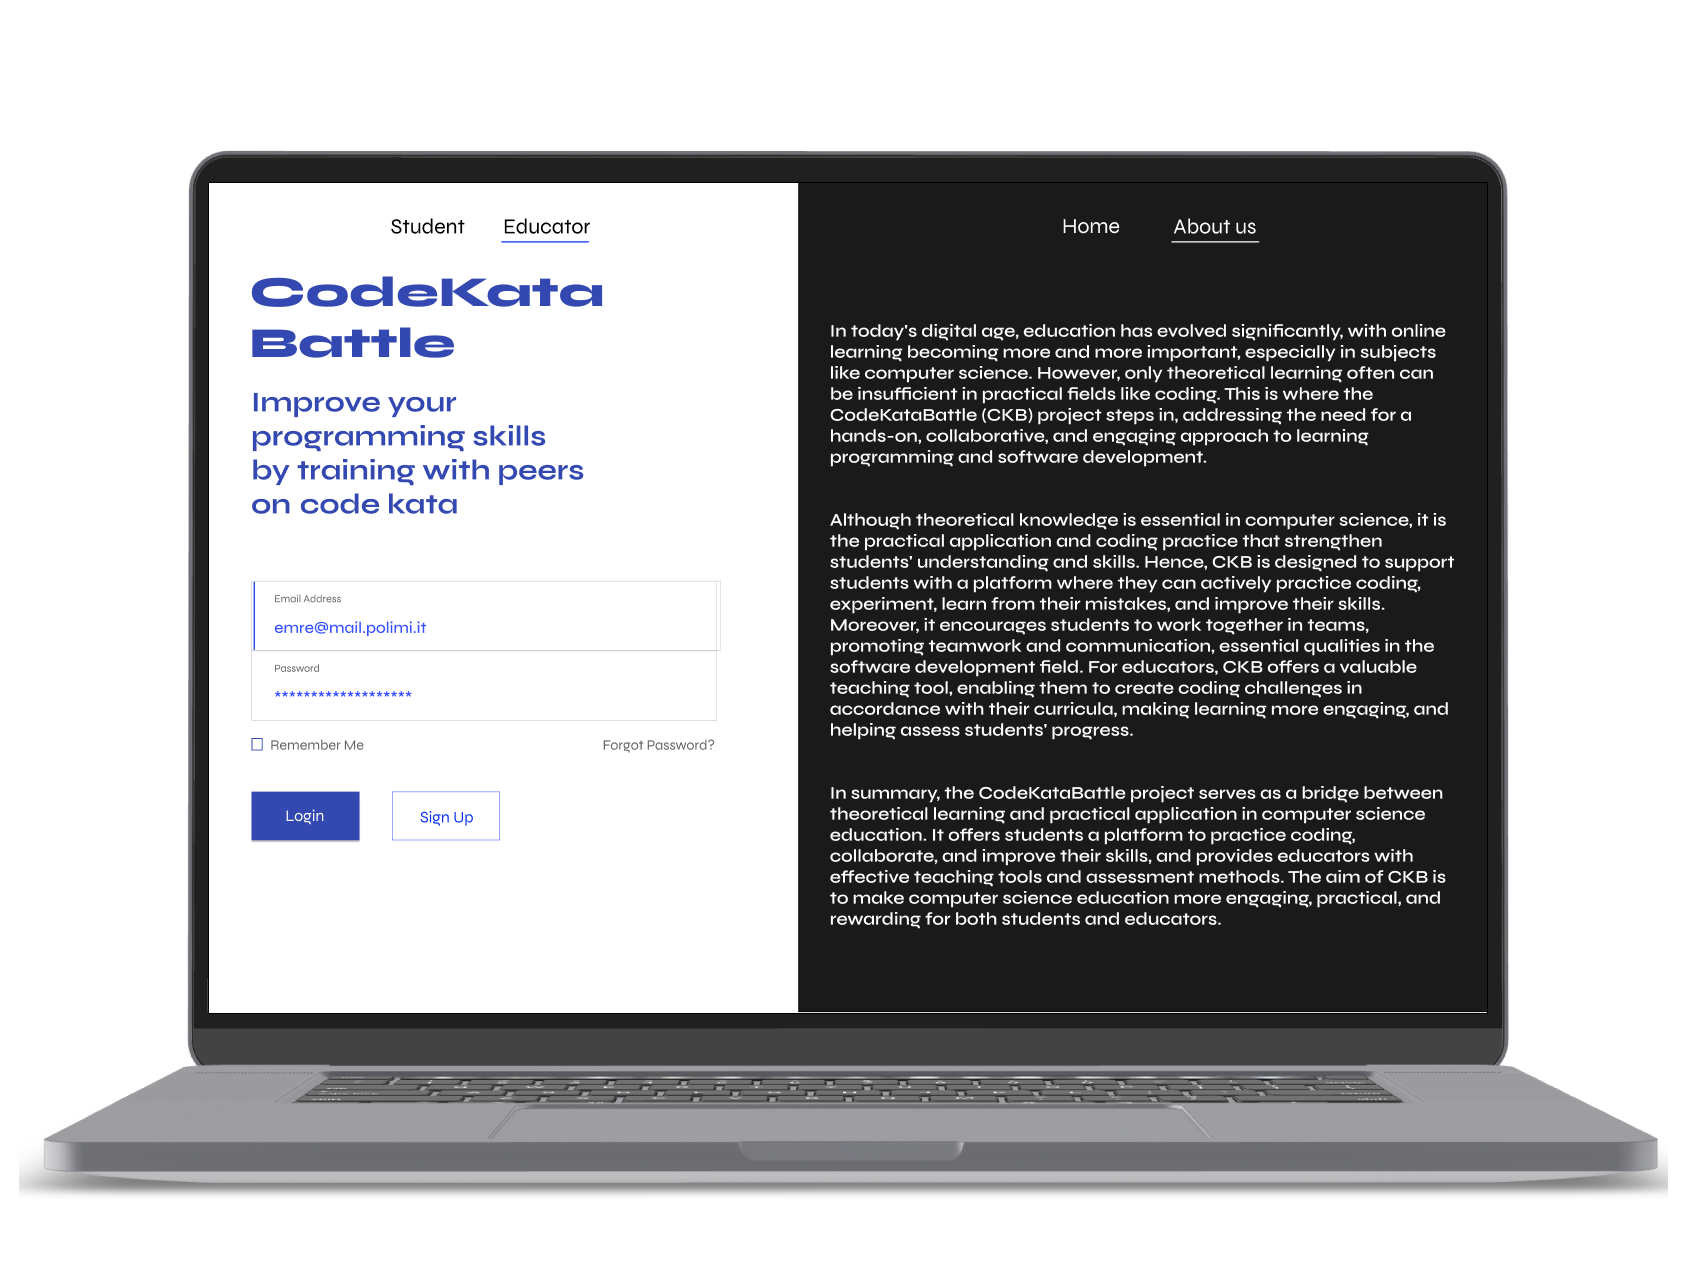
\includegraphics[scale=0.13]{Images/ui-ux/educator_login.png}
\end{center}
    \begin{center}
        (b) $UI_{2}$ Login Screens
    \end{center}

\newpage
\begin{center}
    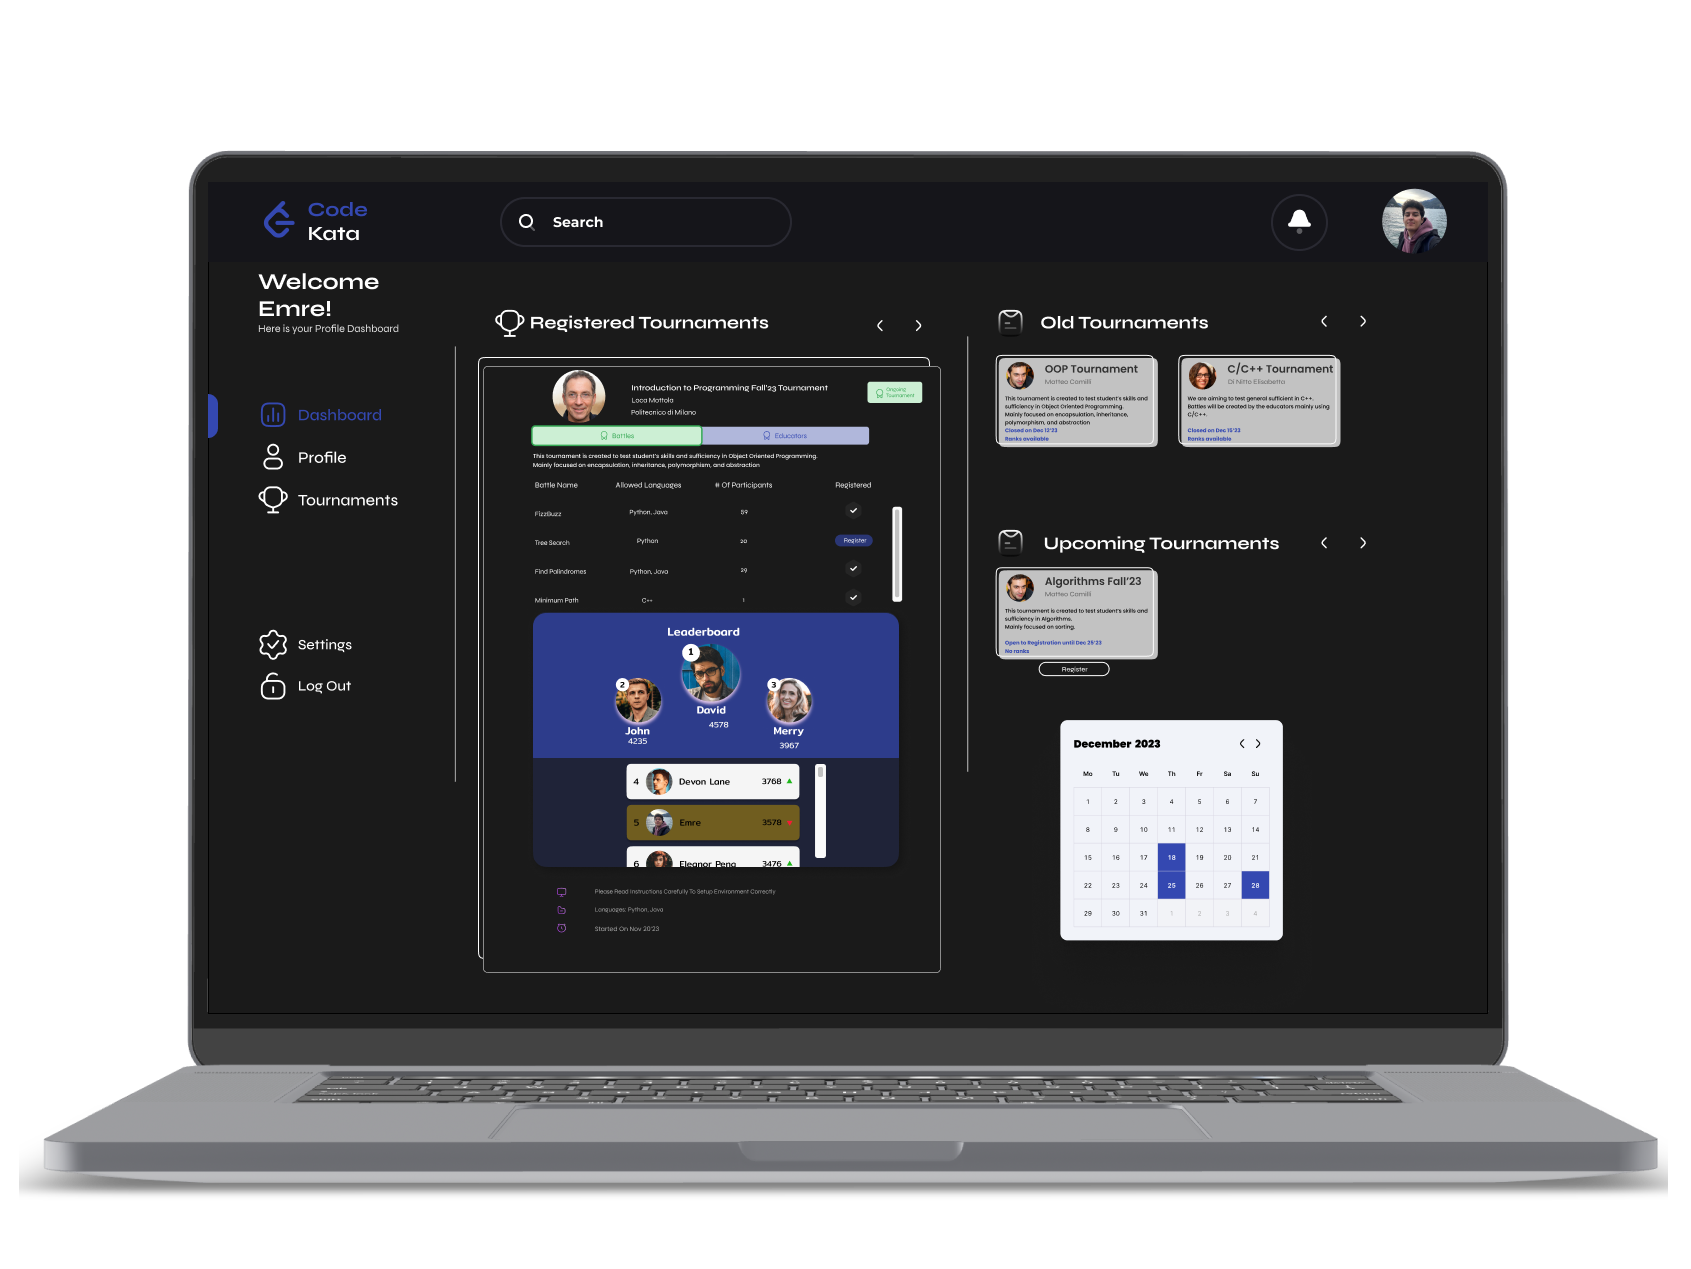
\includegraphics[scale=0.13]{Images/ui-ux/student_dashboard_1.png}
    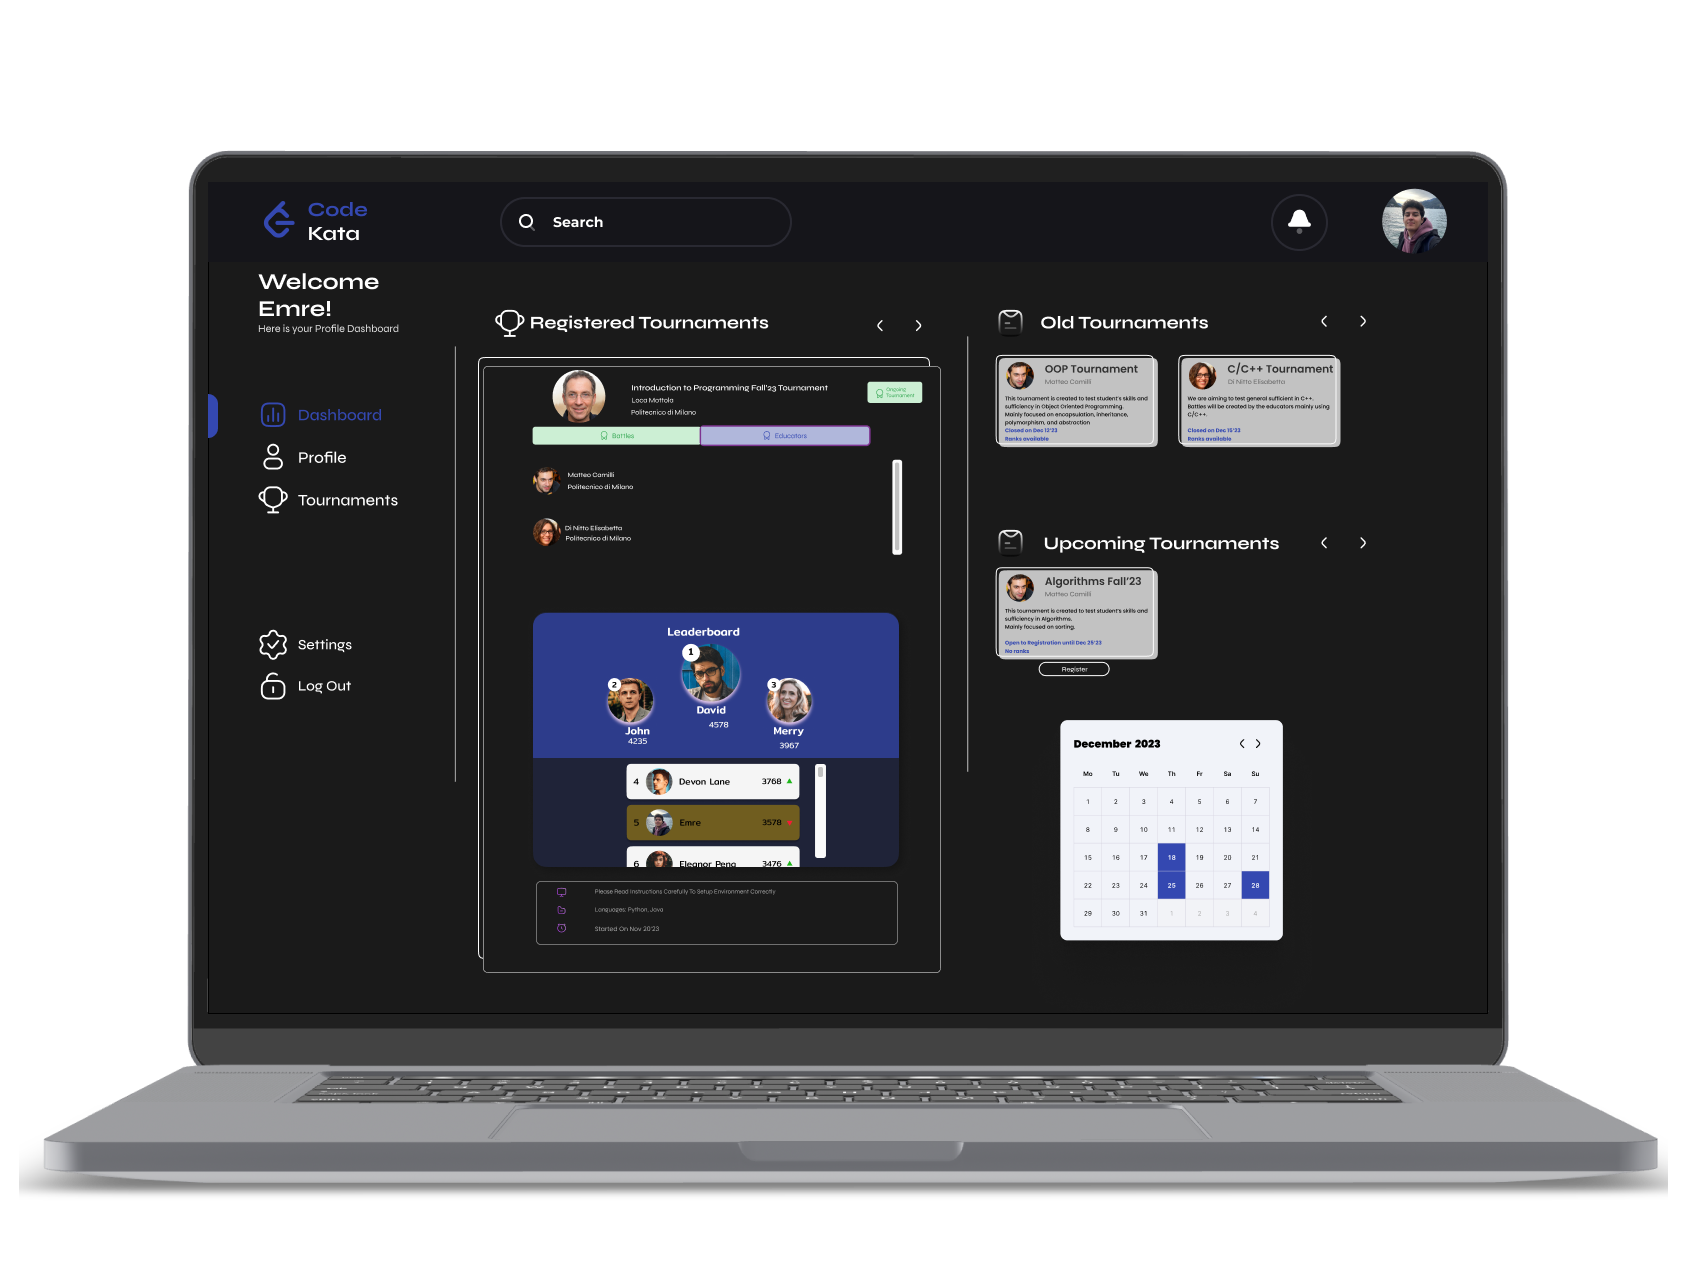
\includegraphics[scale=0.13]{Images/ui-ux/student_dashboard_2.png}
        (c) $UI_{3}$ Student Dashboard
\end{center}
\begin{center}
    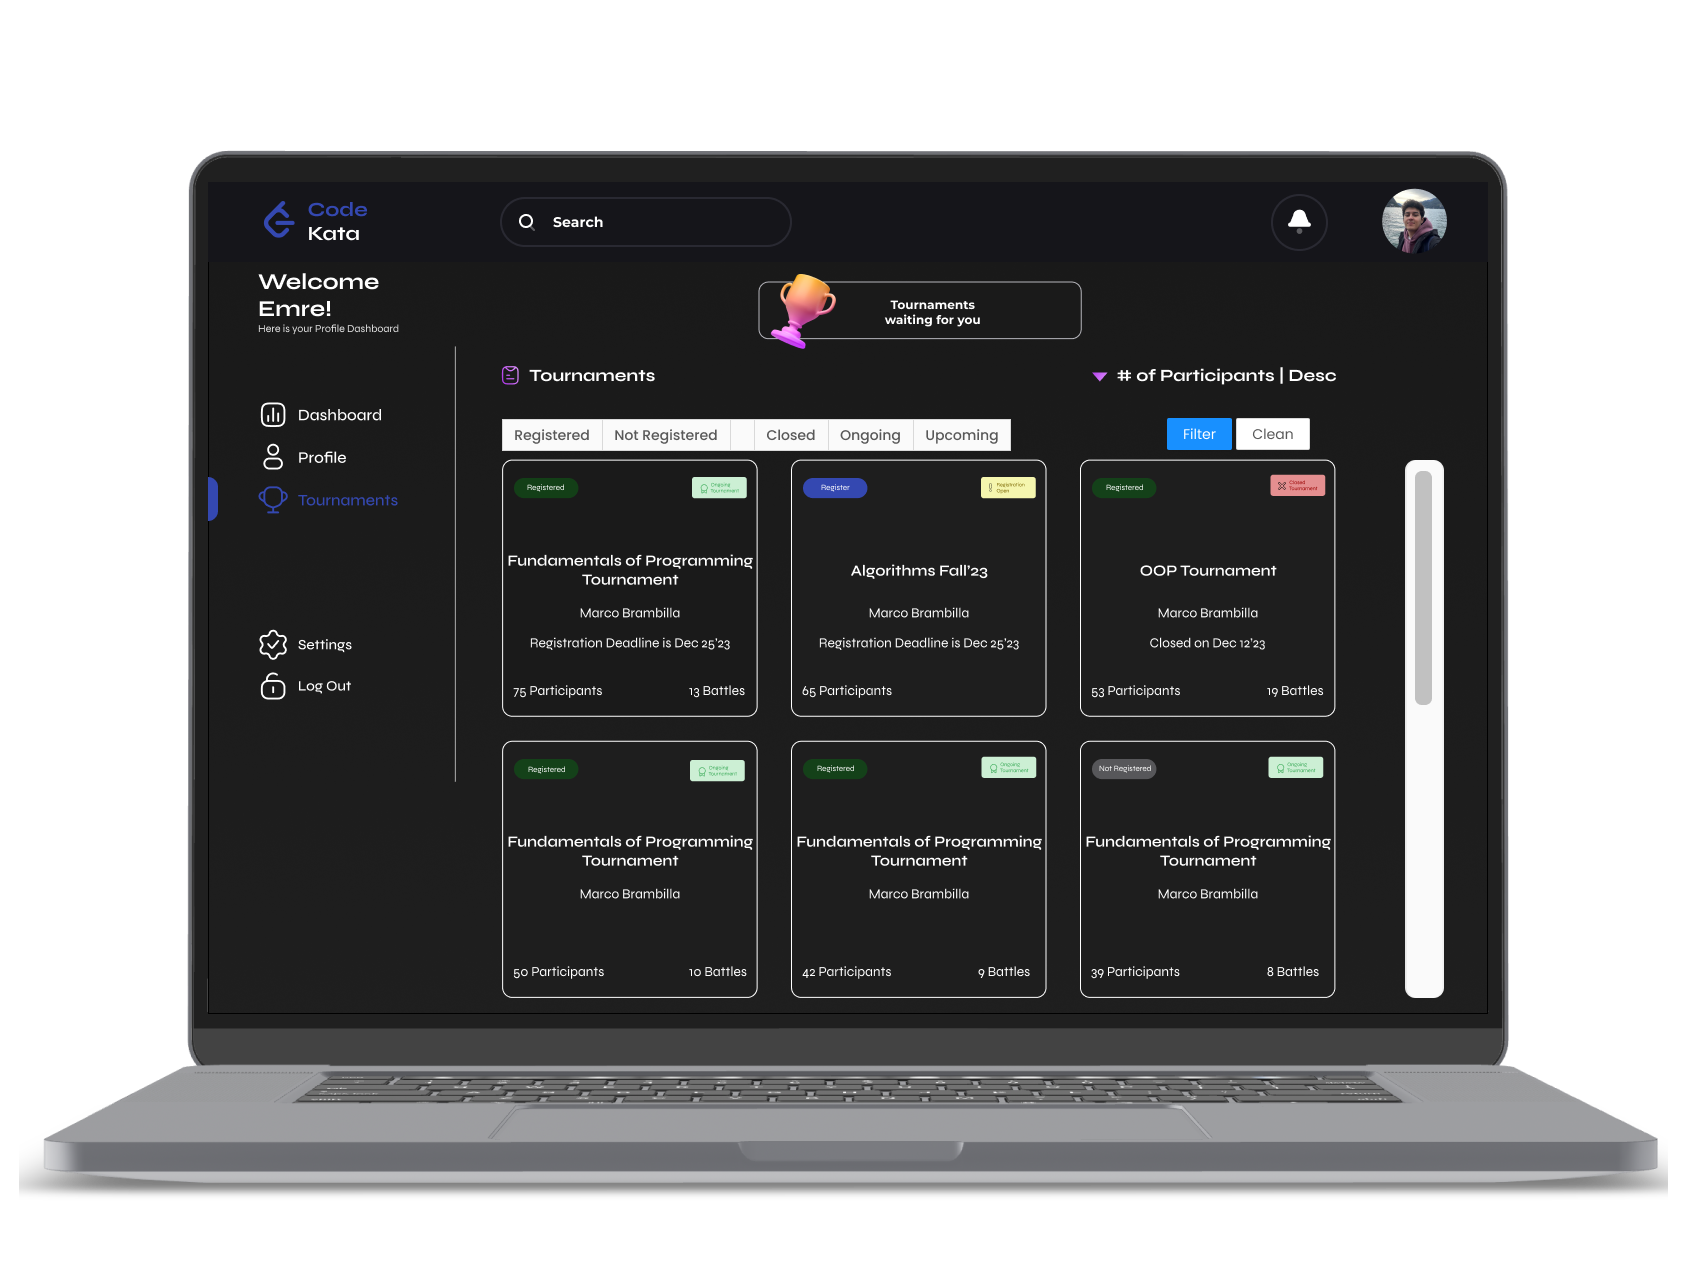
\includegraphics[scale=0.13]{Images/ui-ux/student_tournaments_1.png}
    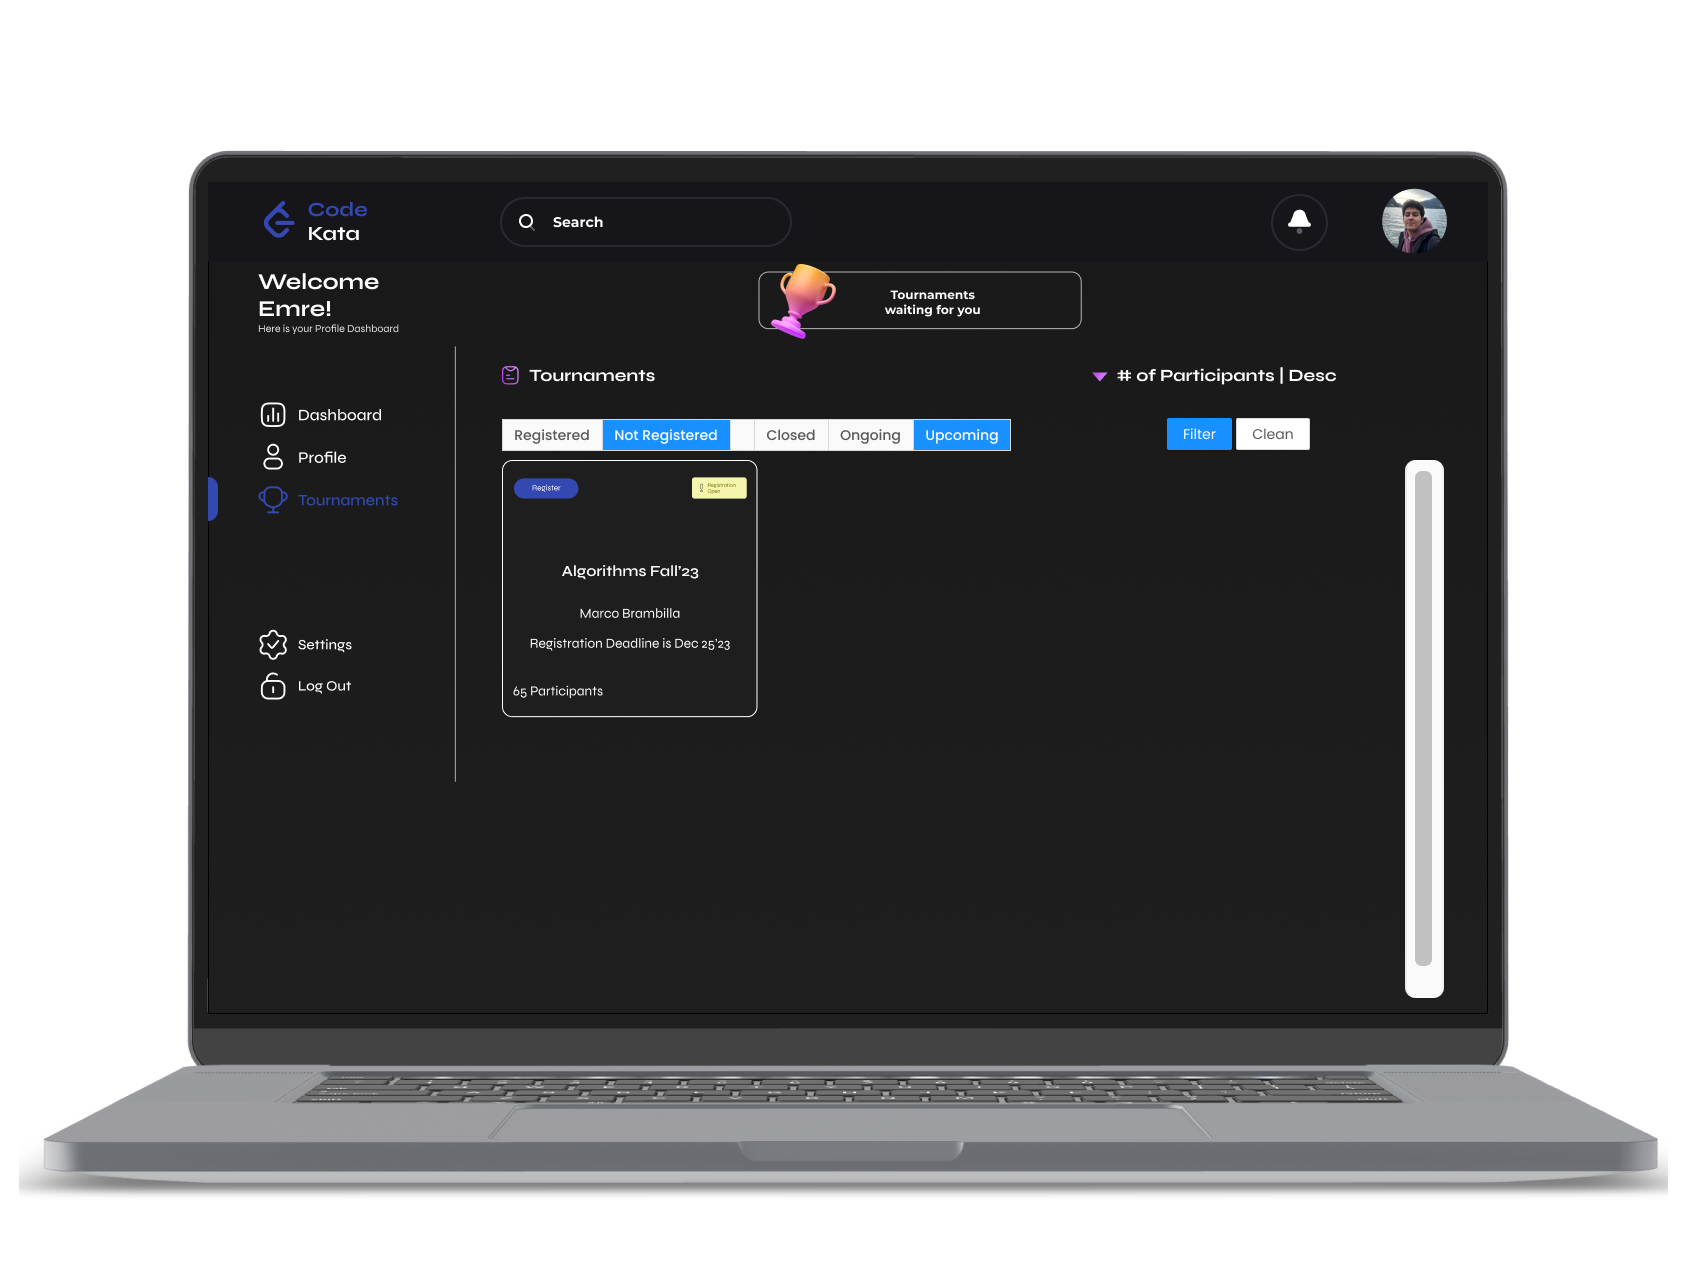
\includegraphics[scale=0.13]{Images/ui-ux/student_tournaments_2.png}    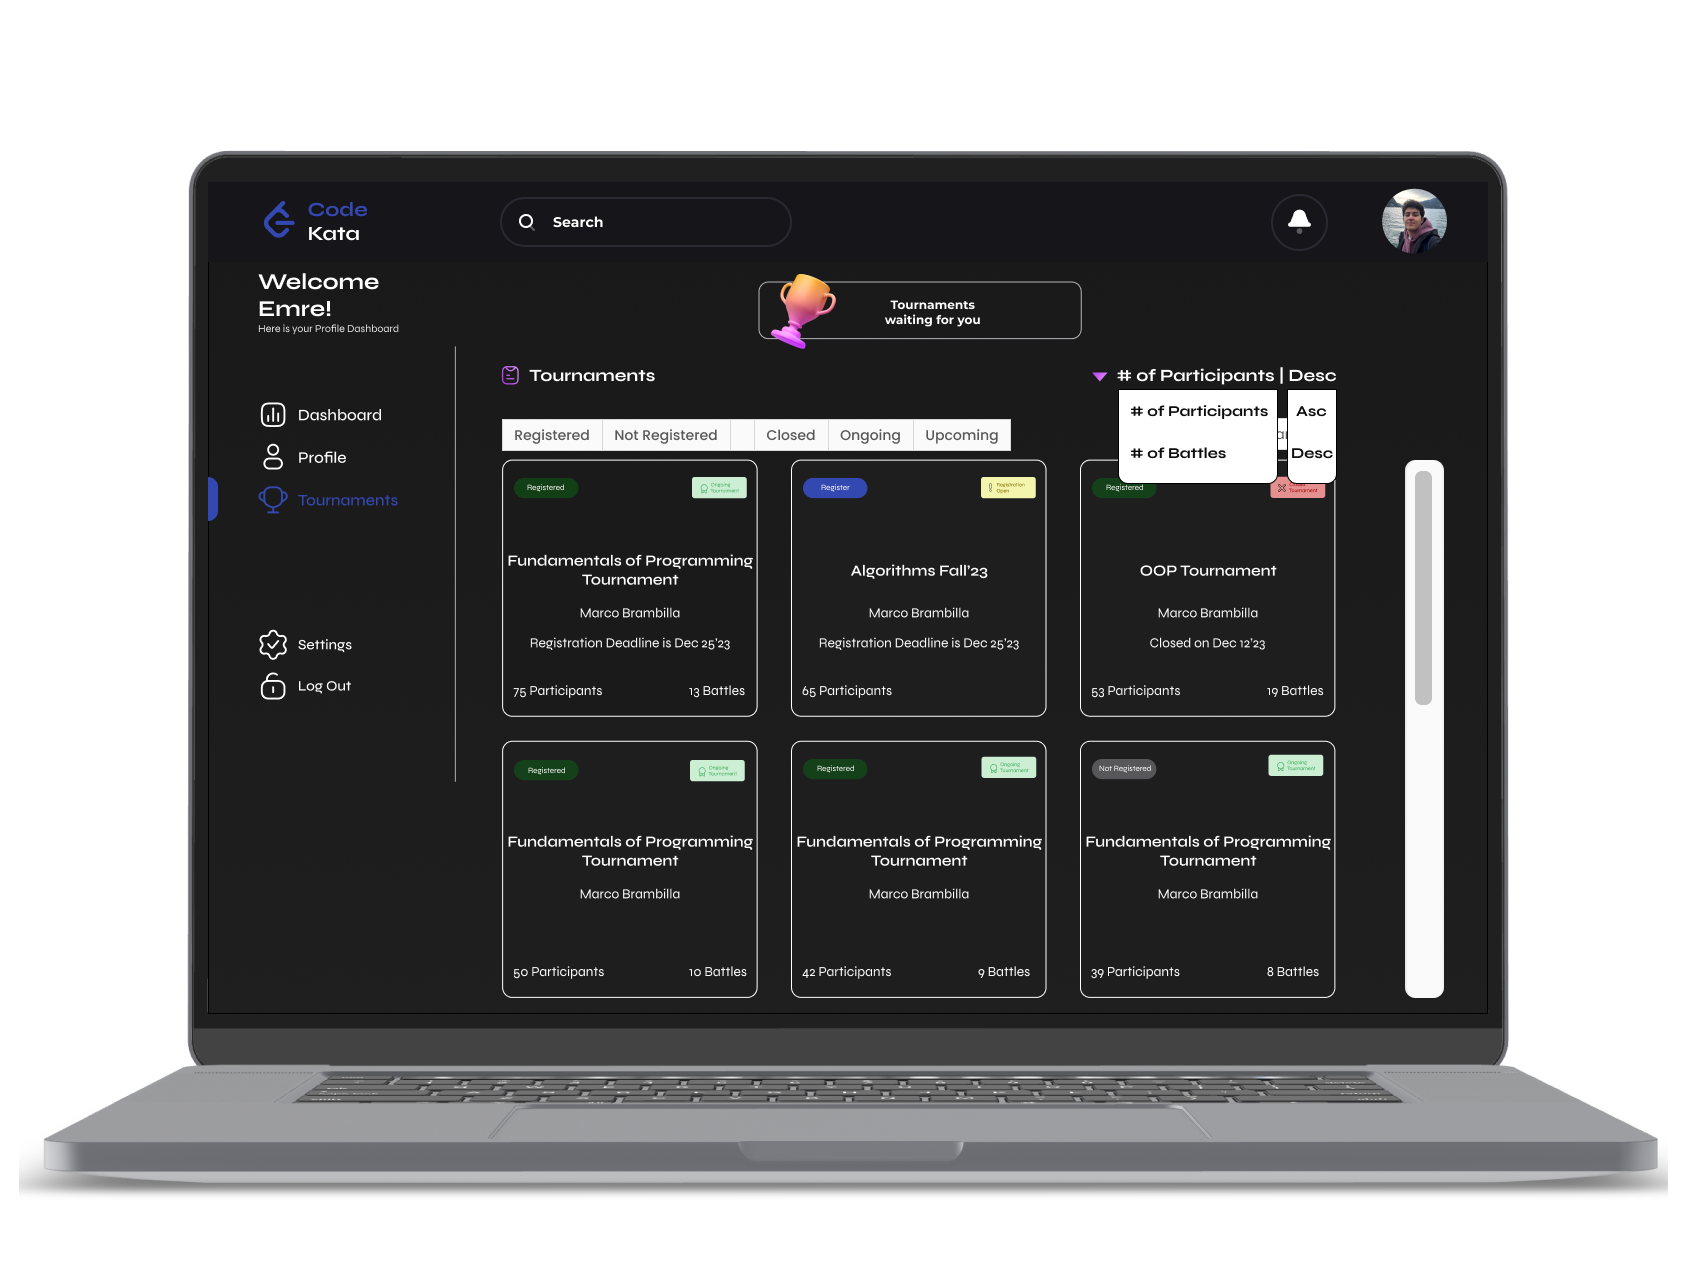
\includegraphics[scale=0.13]{Images/ui-ux/student_tournaments_3.png}    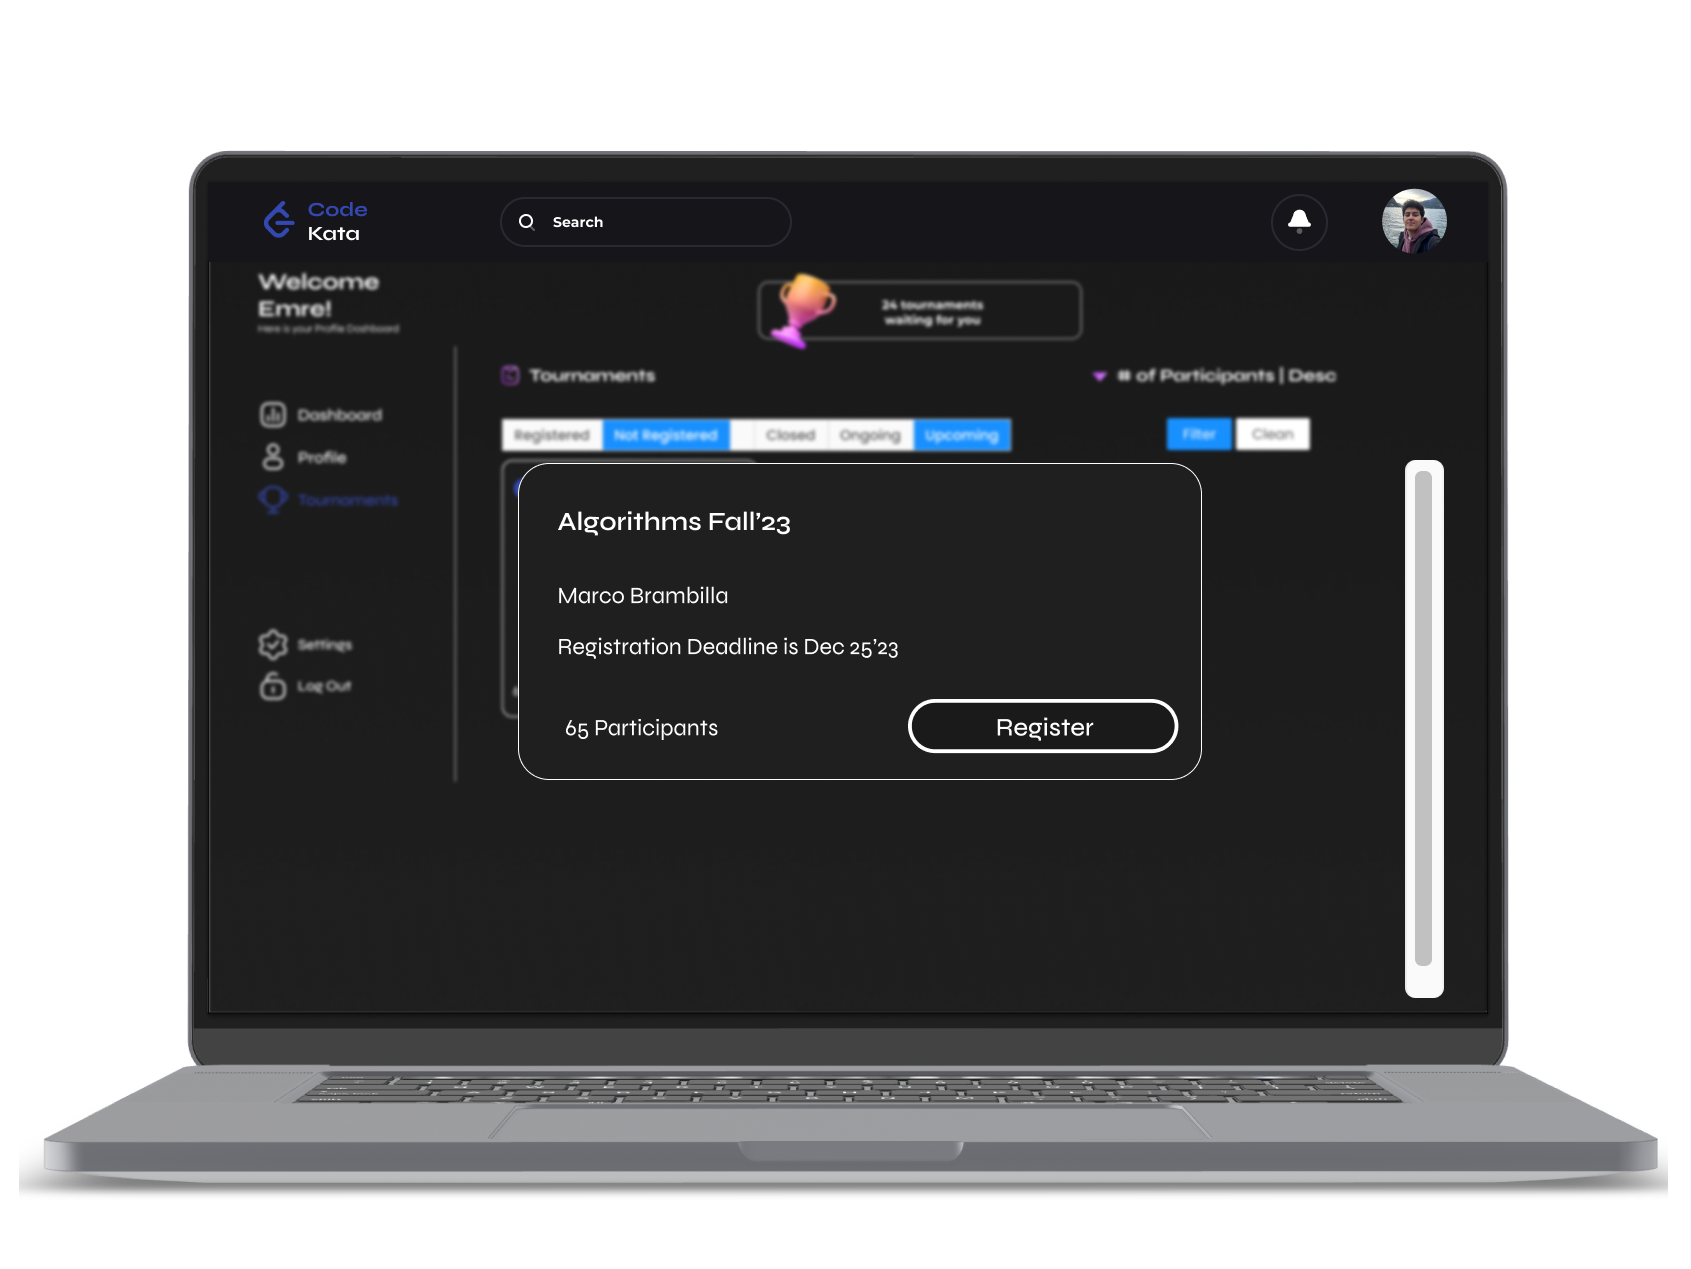
\includegraphics[scale=0.13]{Images/ui-ux/student_tournaments_4.png}
        (d) $UI_{4}$ Student Tournaments Page
\end{center}

\begin{center}
    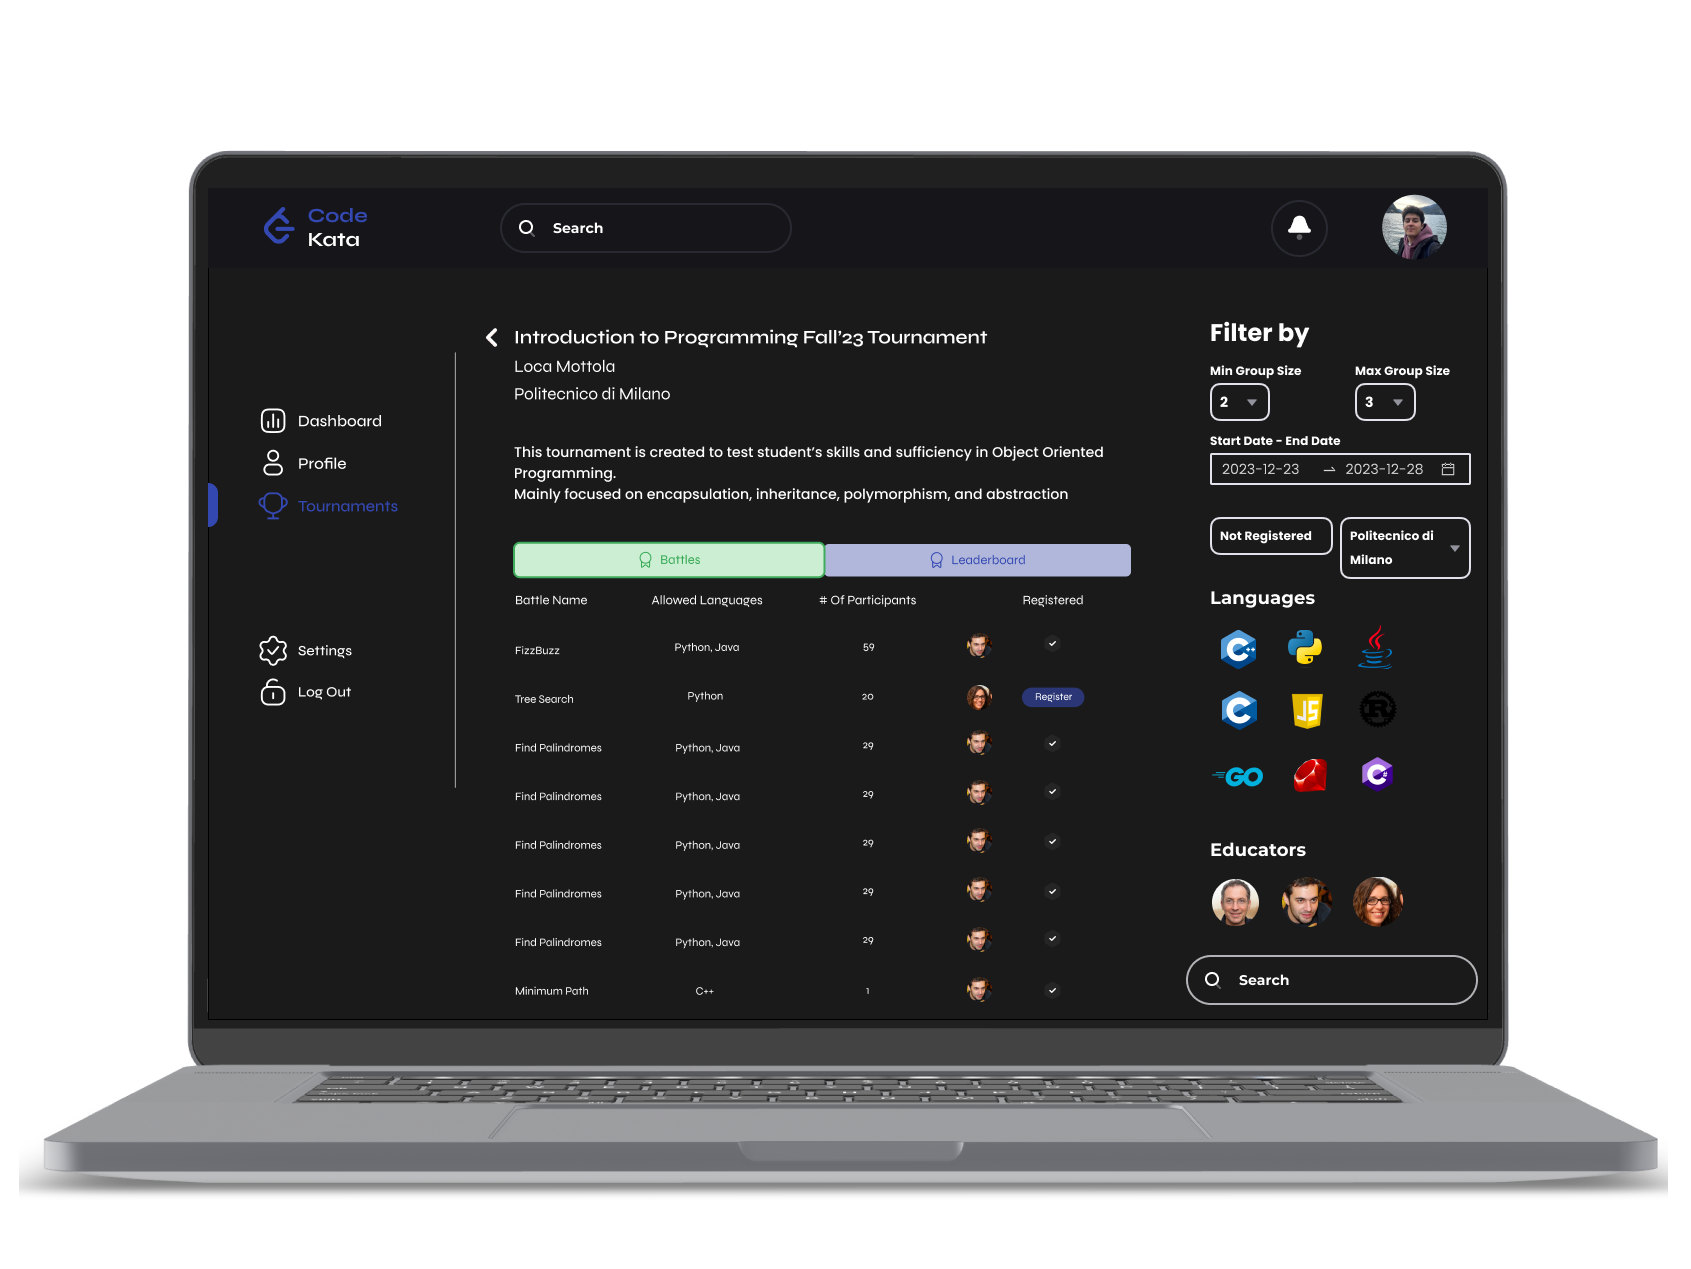
\includegraphics[scale=0.13]{Images/ui-ux/student_tournament_1.png}
    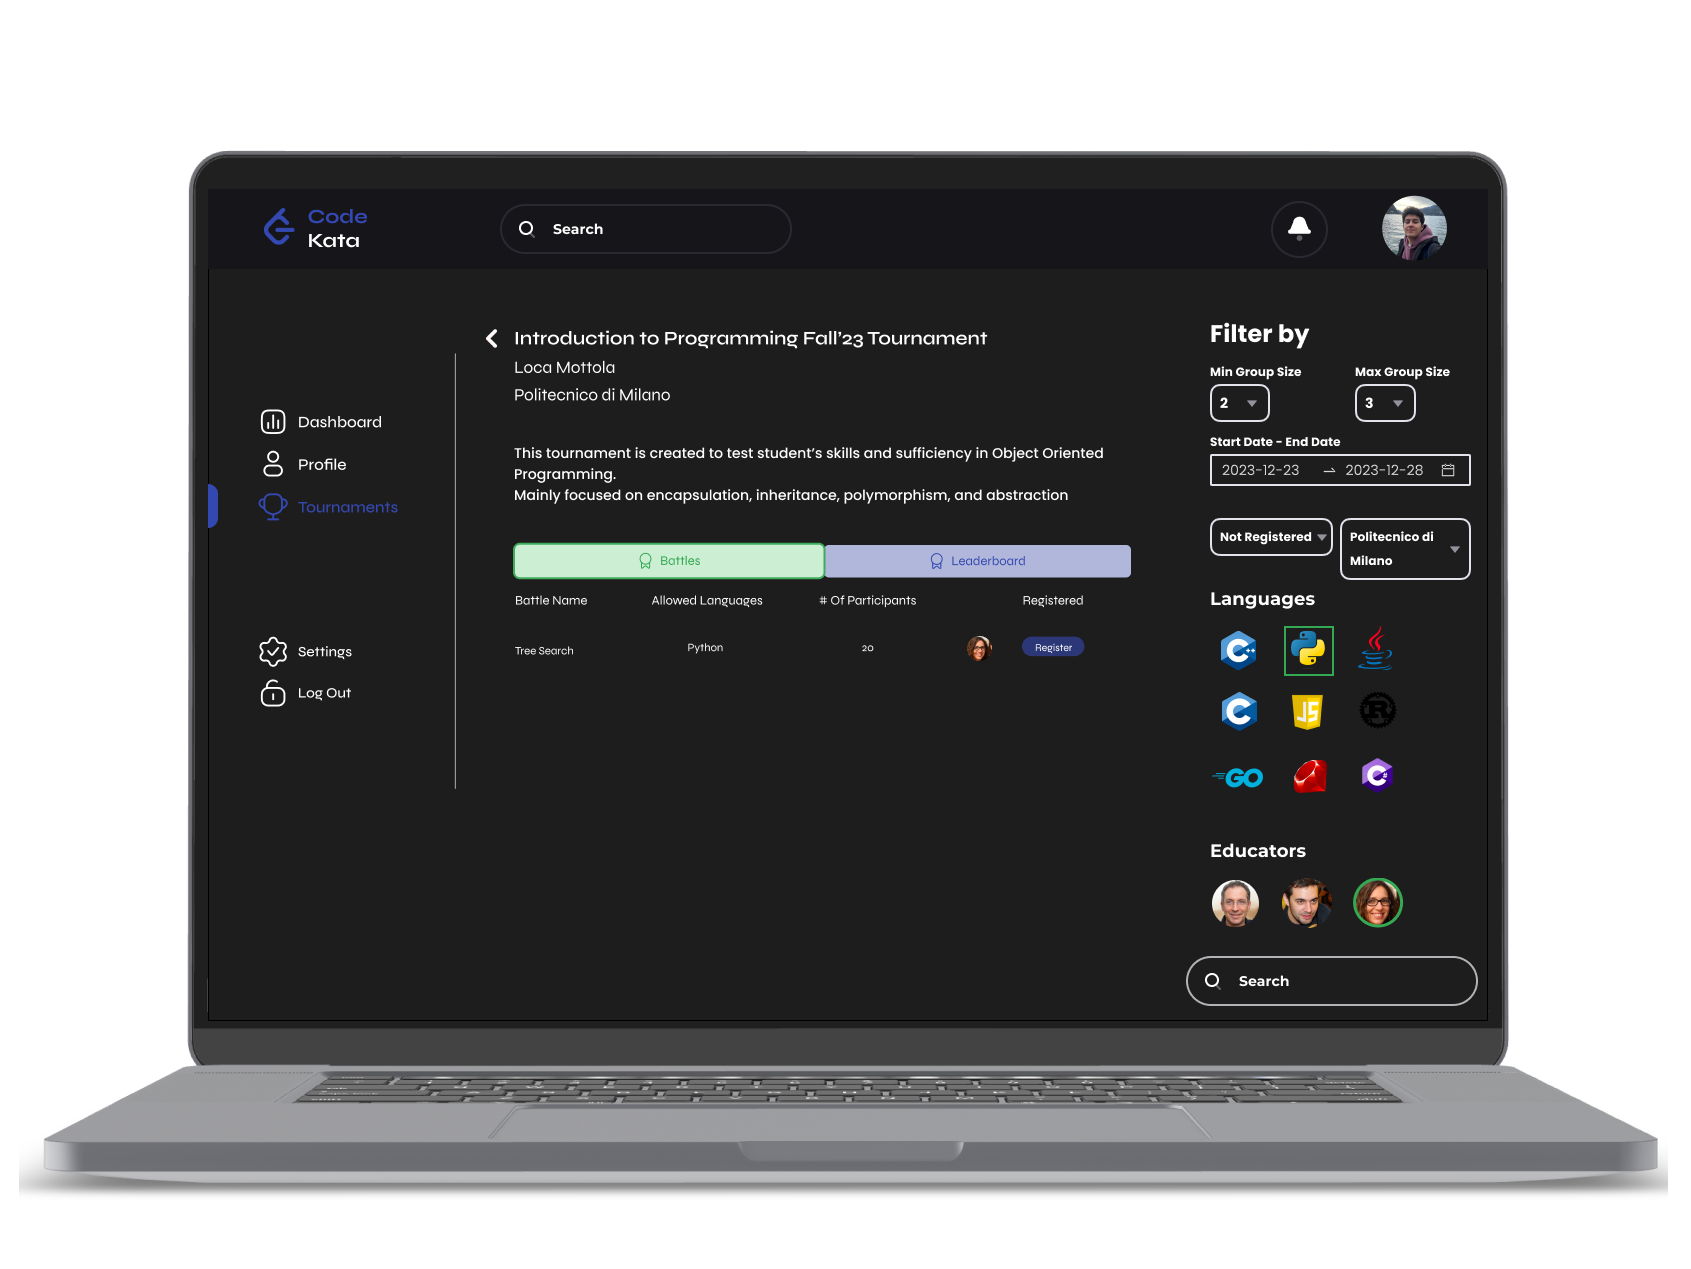
\includegraphics[scale=0.13]{Images/ui-ux/student_tournament_2.png}    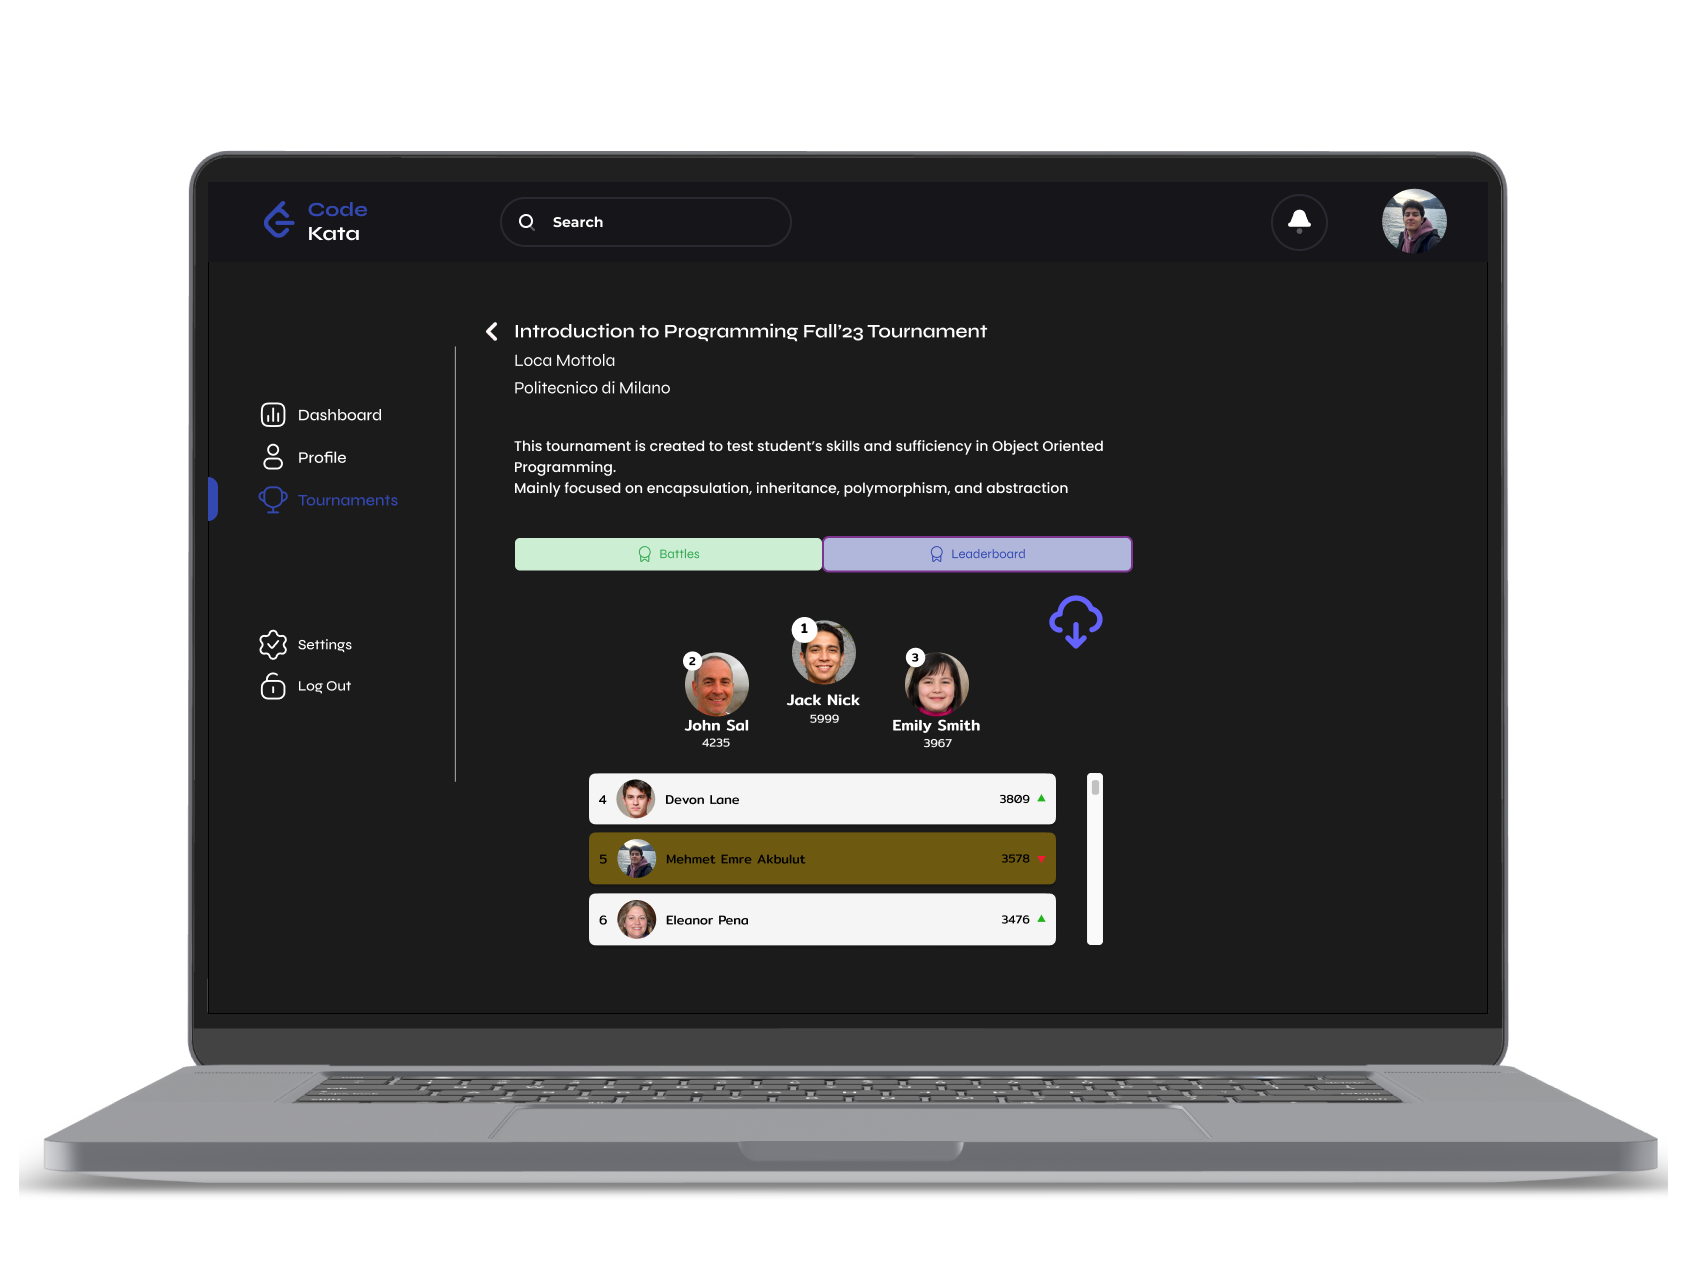
\includegraphics[scale=0.13]{Images/ui-ux/student_tournament_3.png} 
    \\ (e) $UI_{5}$ Student visits a Tournament 
\end{center}
\newpage
\begin{center}
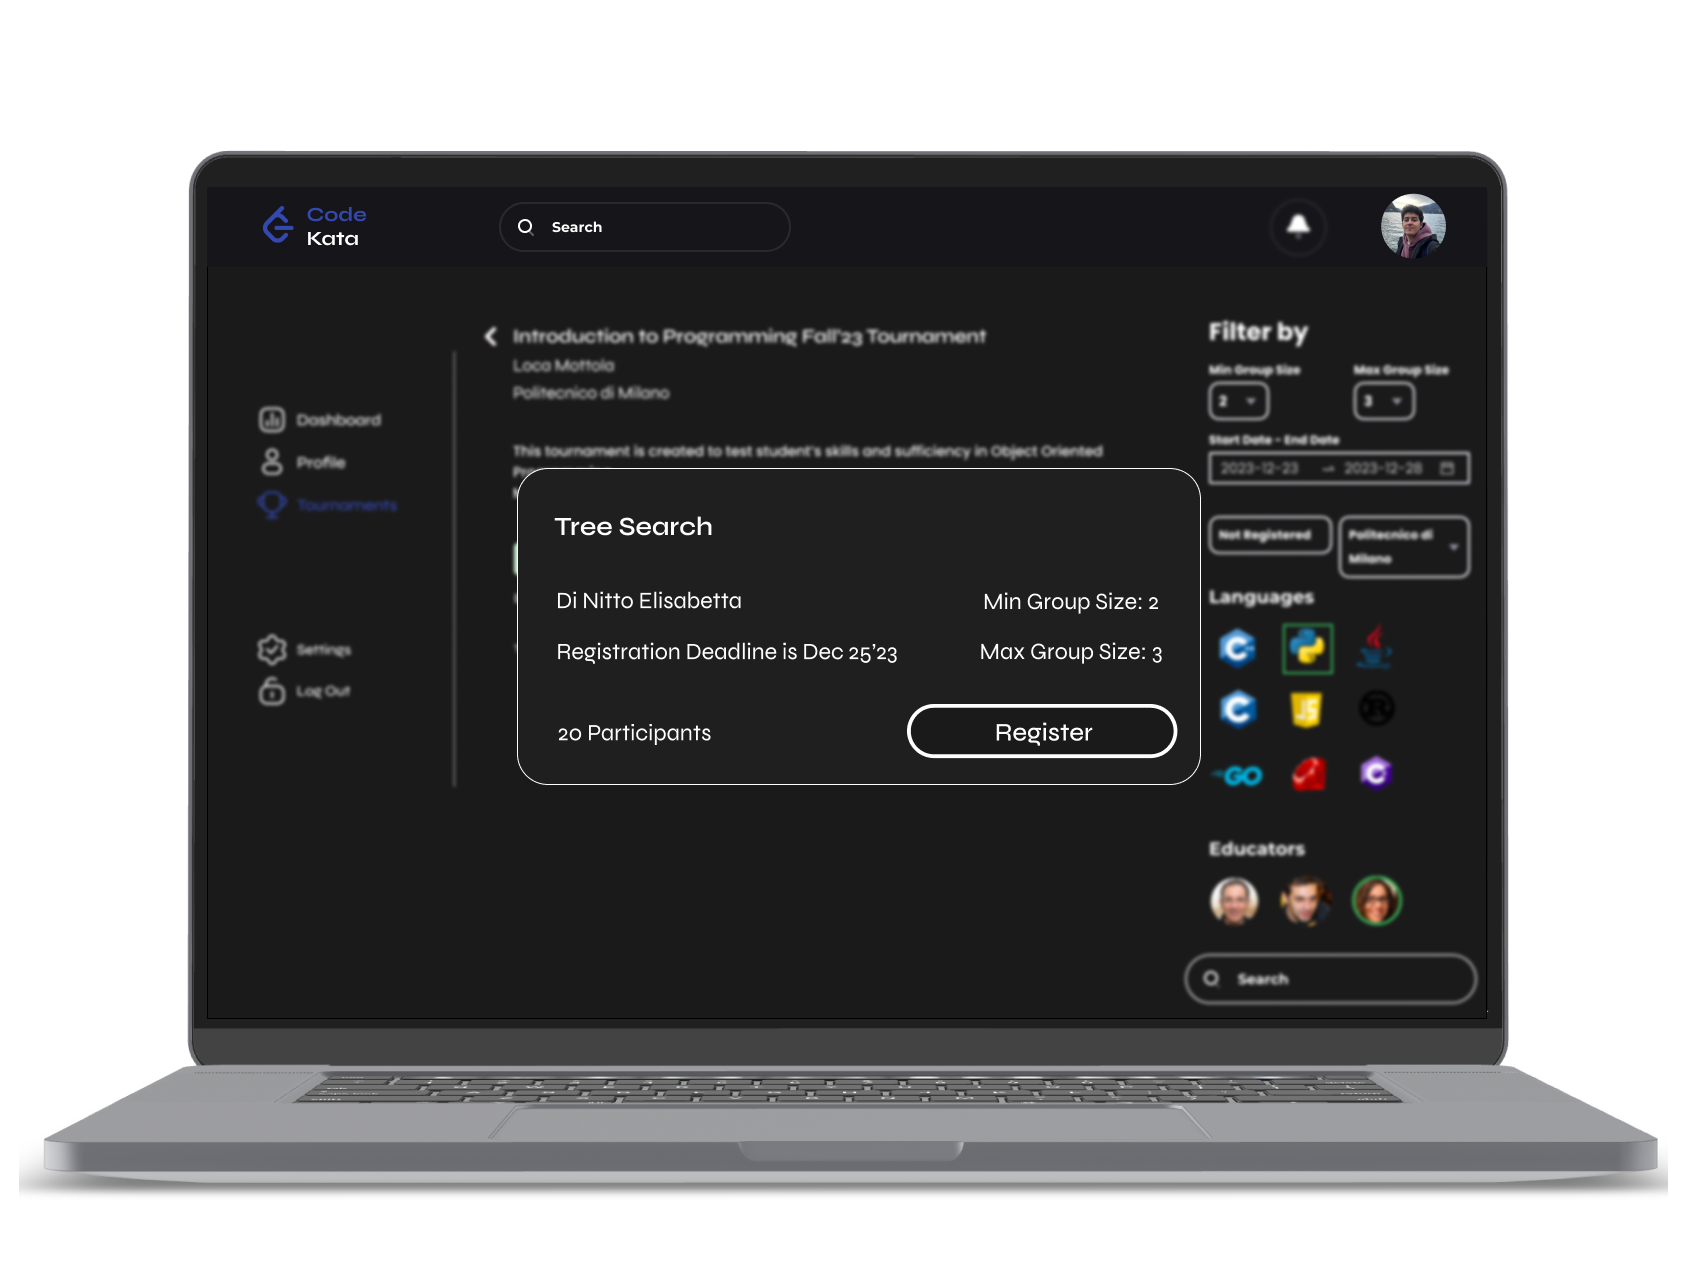
\includegraphics[scale=0.13]{Images/ui-ux/student_battle_register_1.png}
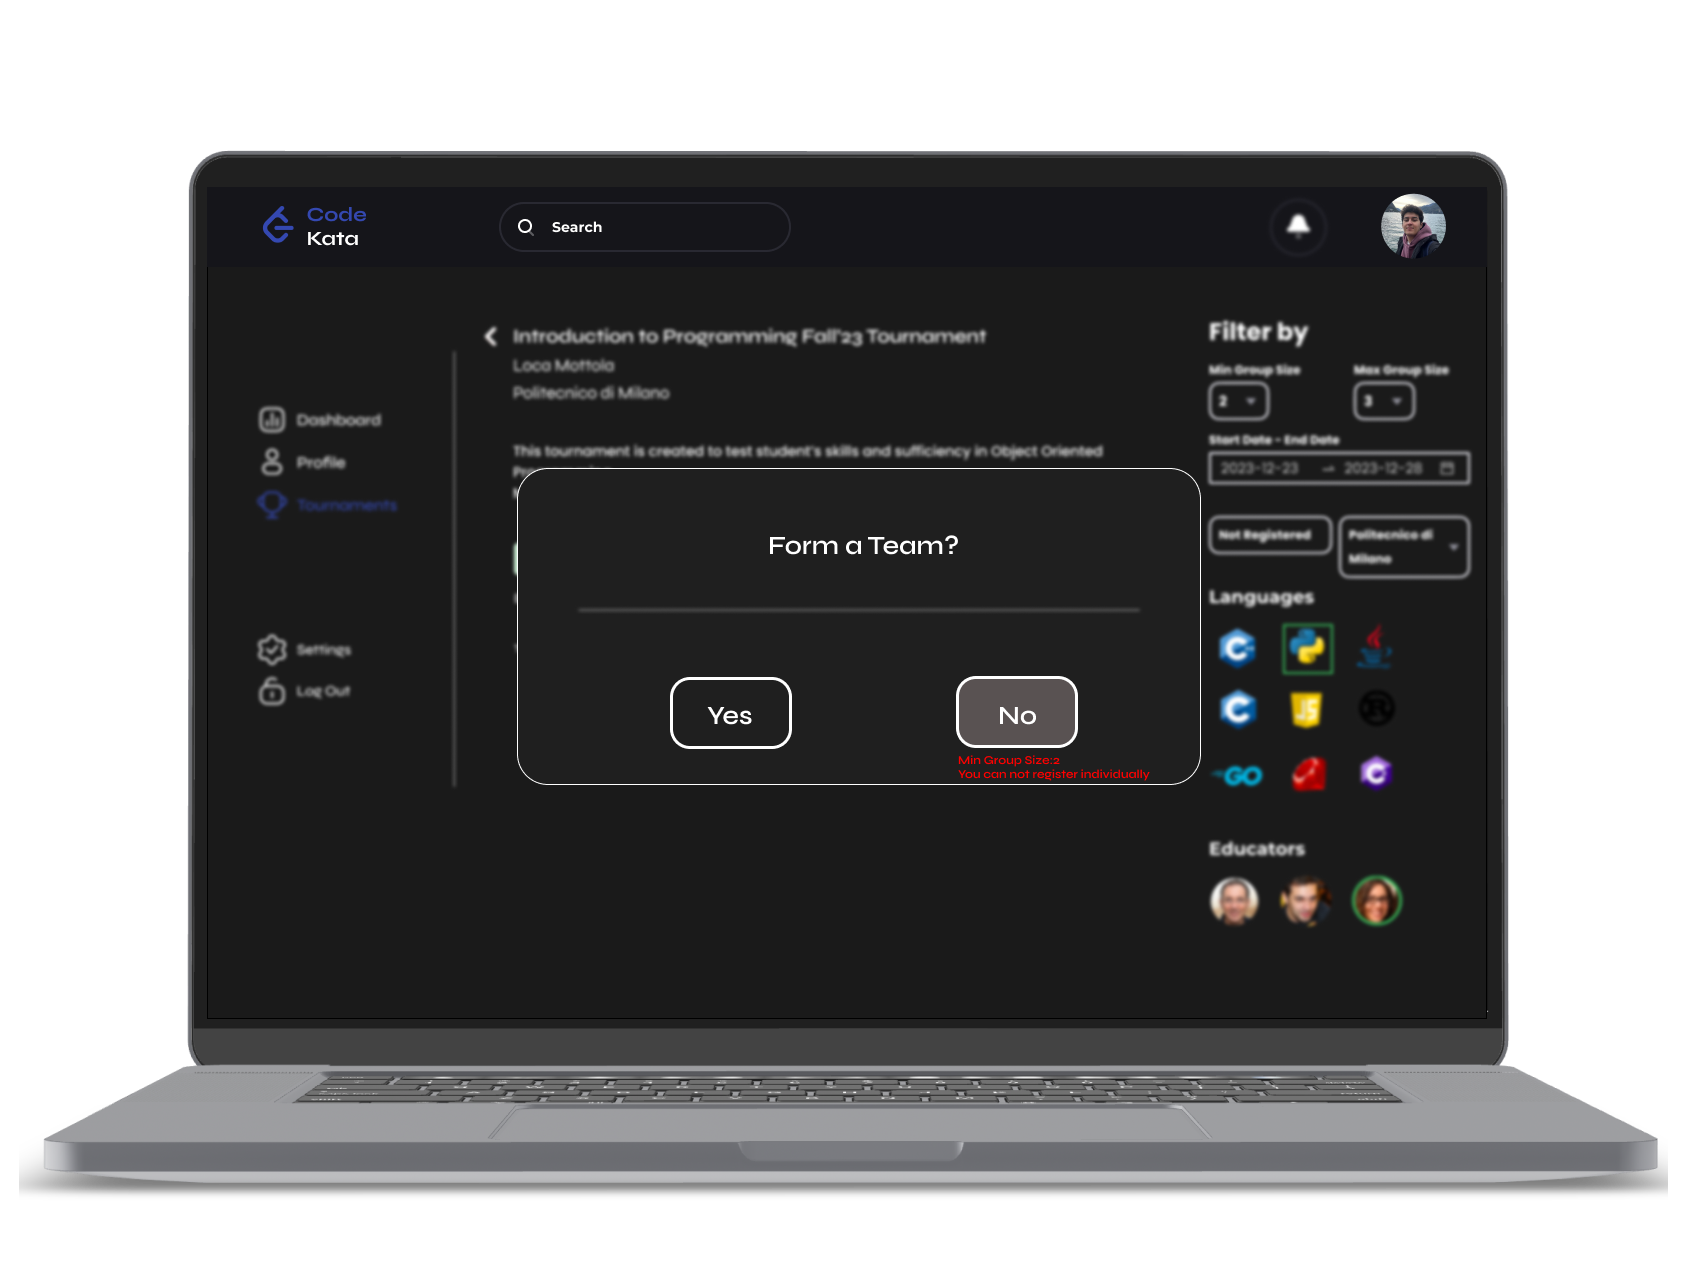
\includegraphics[scale=0.13]{Images/ui-ux/student_battle_register_2.png}
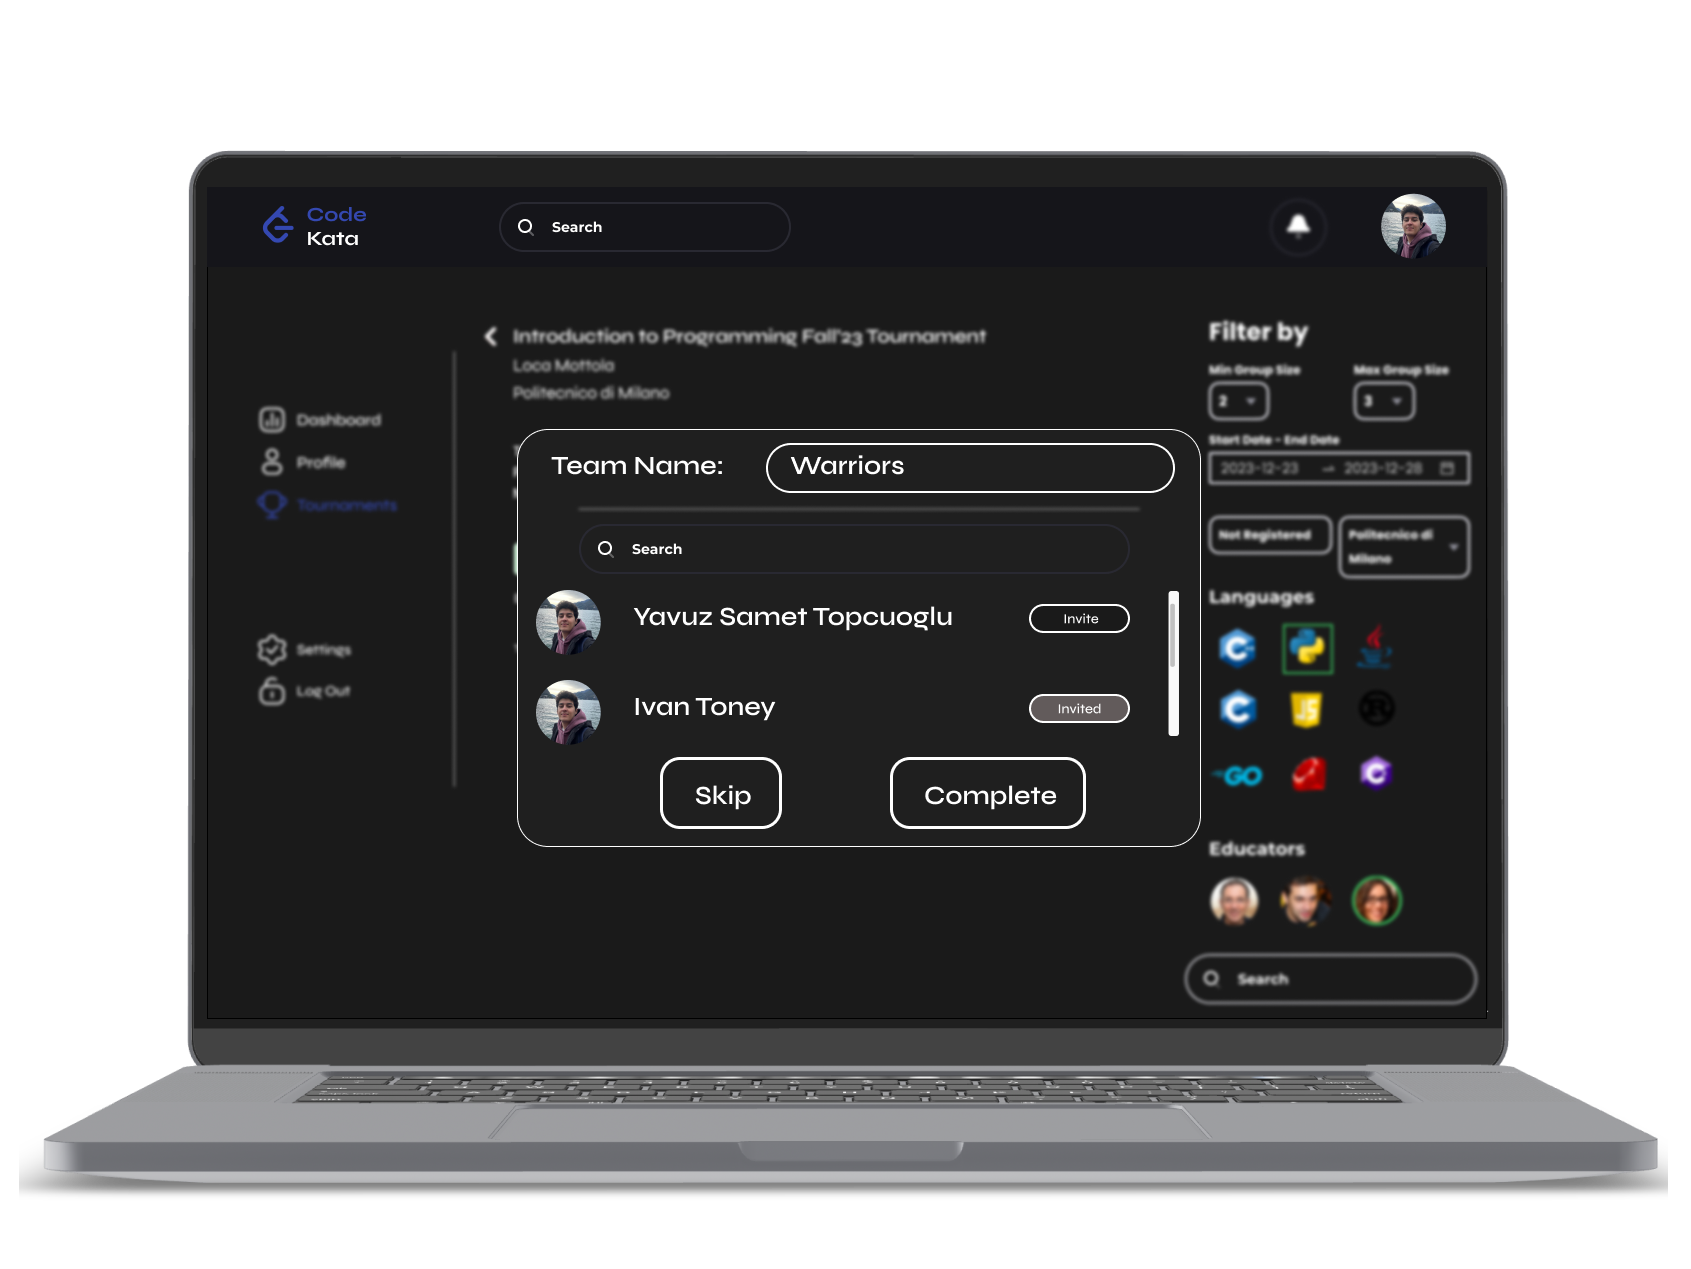
\includegraphics[scale=0.13]{Images/ui-ux/student_battle_register_3.png}
\\ (f) $UI_{6}$  Student Registers Battle 
\end{center}
\newpage
\begin{center}
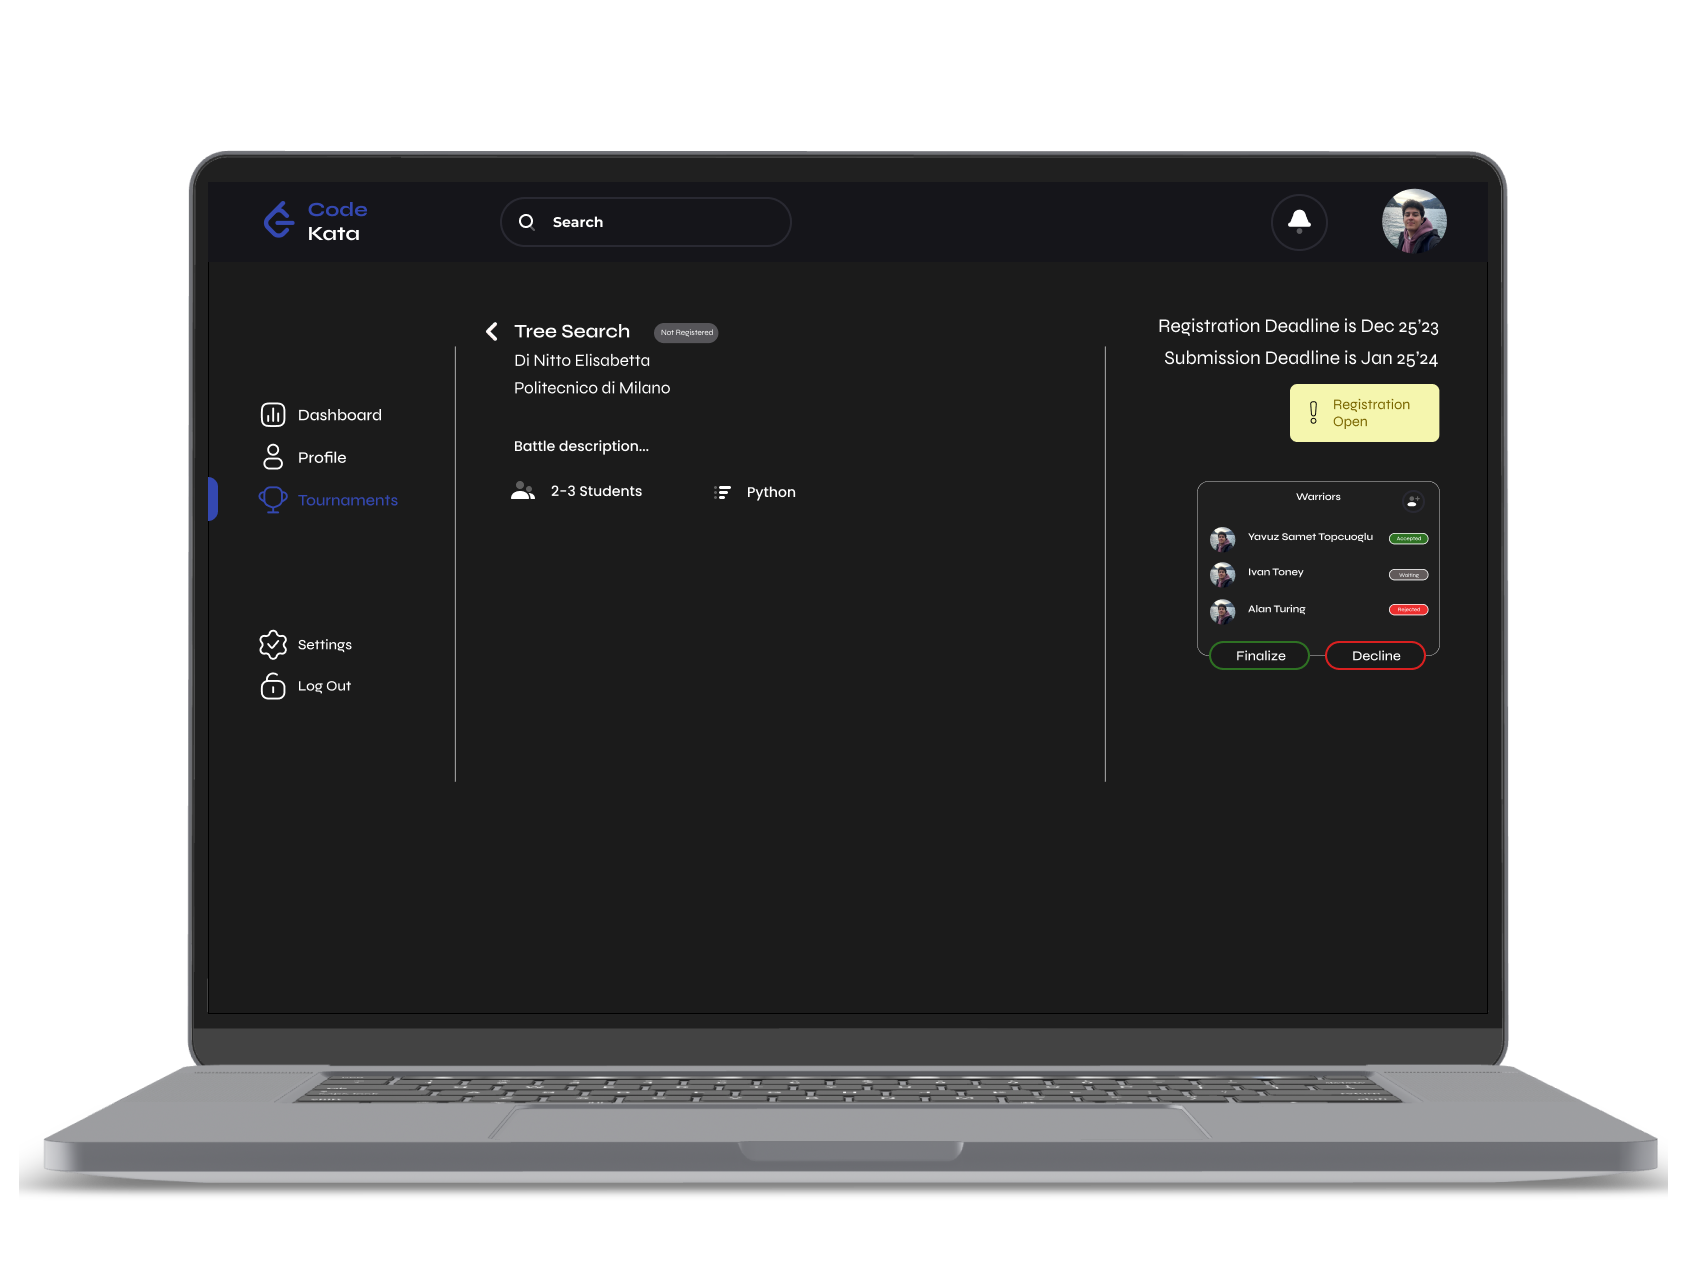
\includegraphics[scale=0.13]{Images/ui-ux/student_battle_1.png}
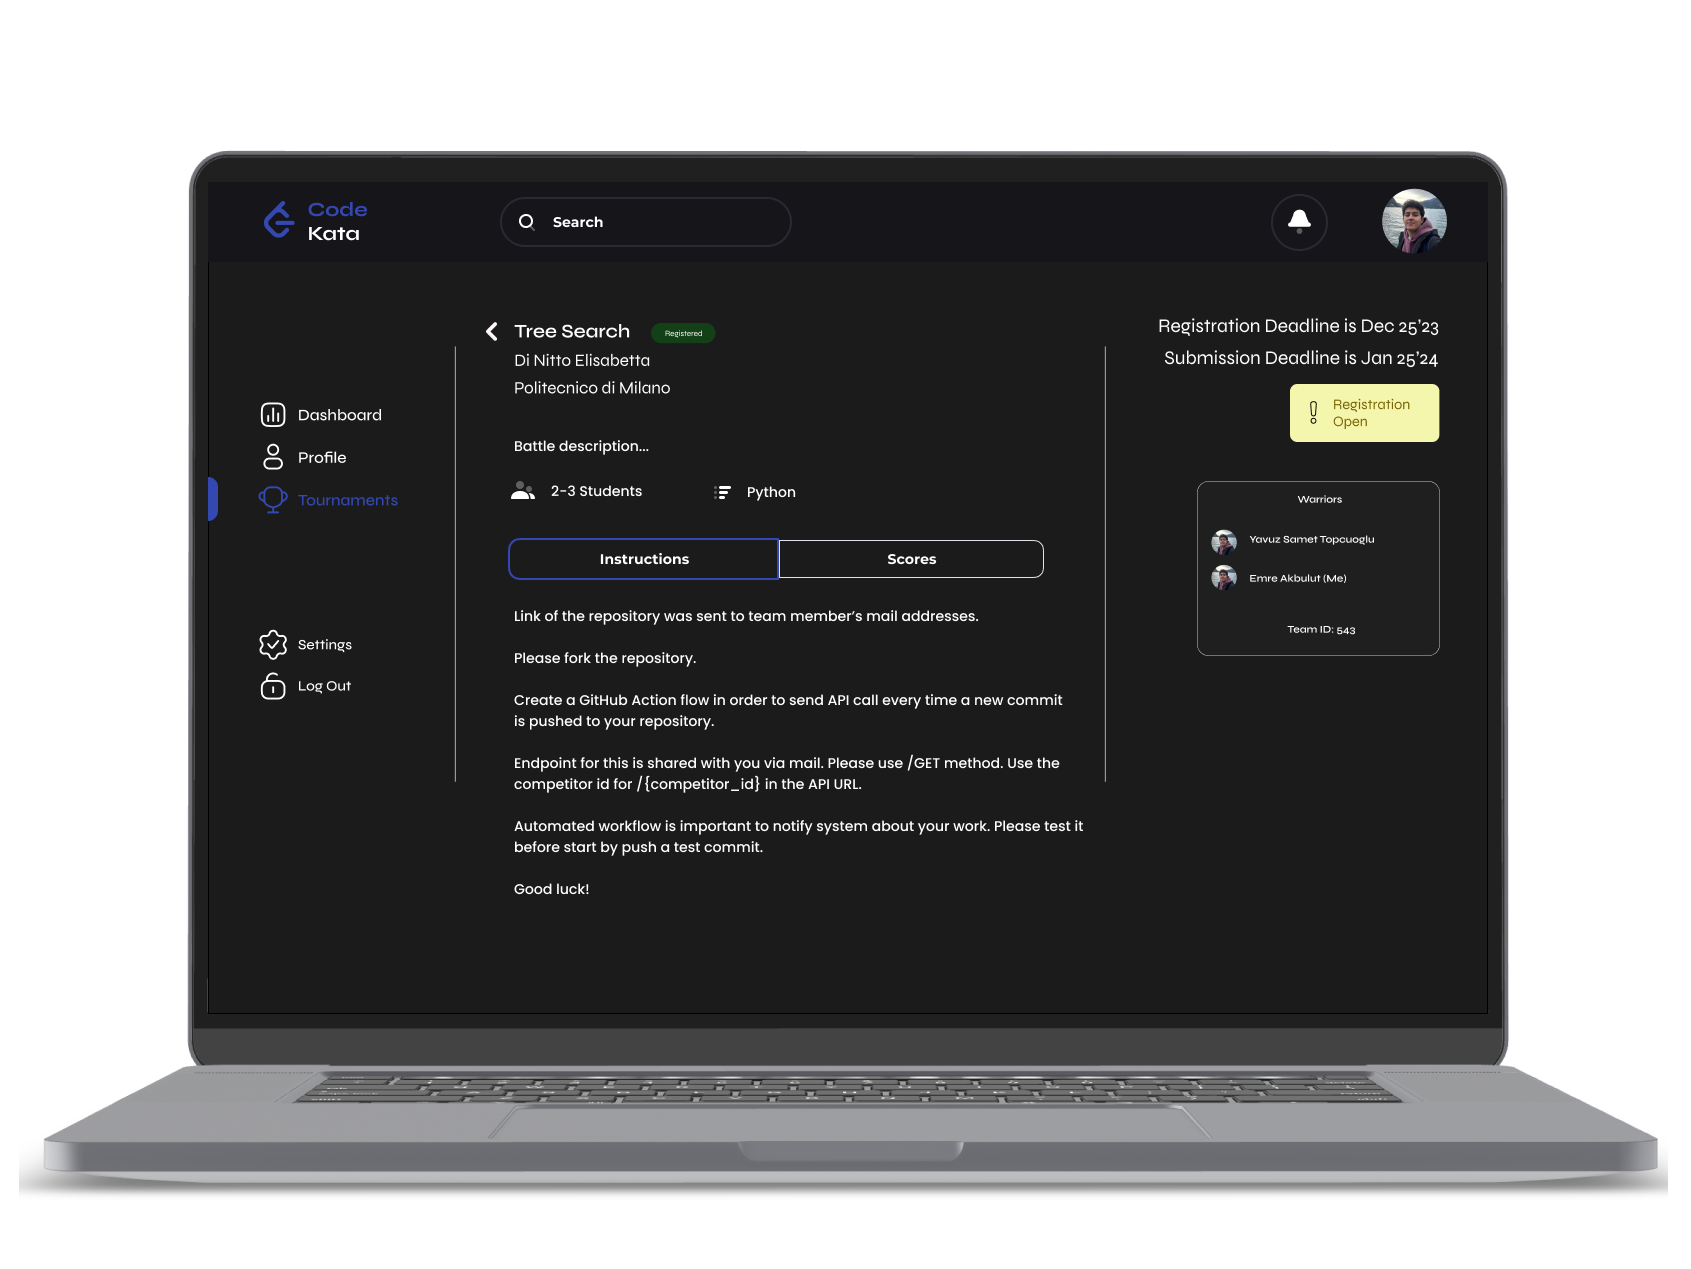
\includegraphics[scale=0.13]{Images/ui-ux/student_battle_2.png}
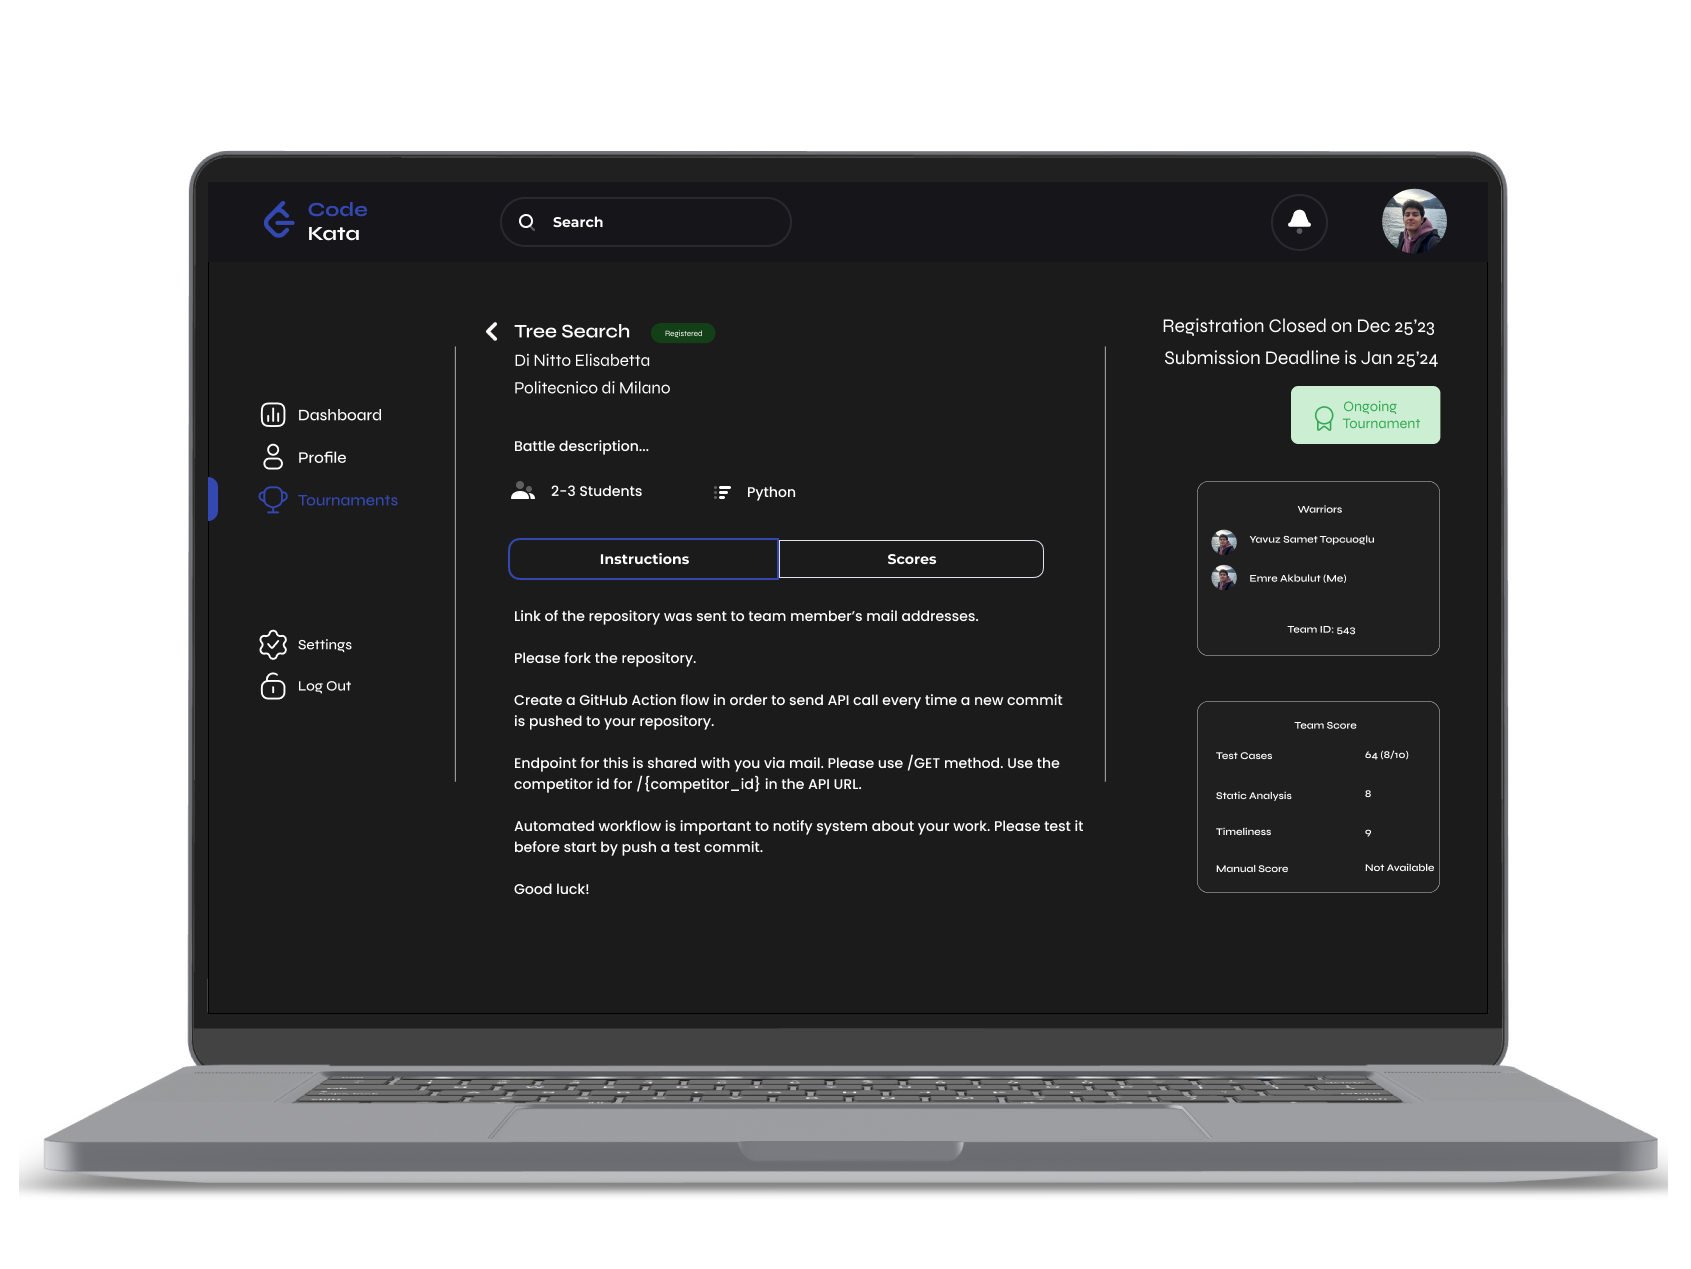
\includegraphics[scale=0.13]{Images/ui-ux/student_battle_3.png}
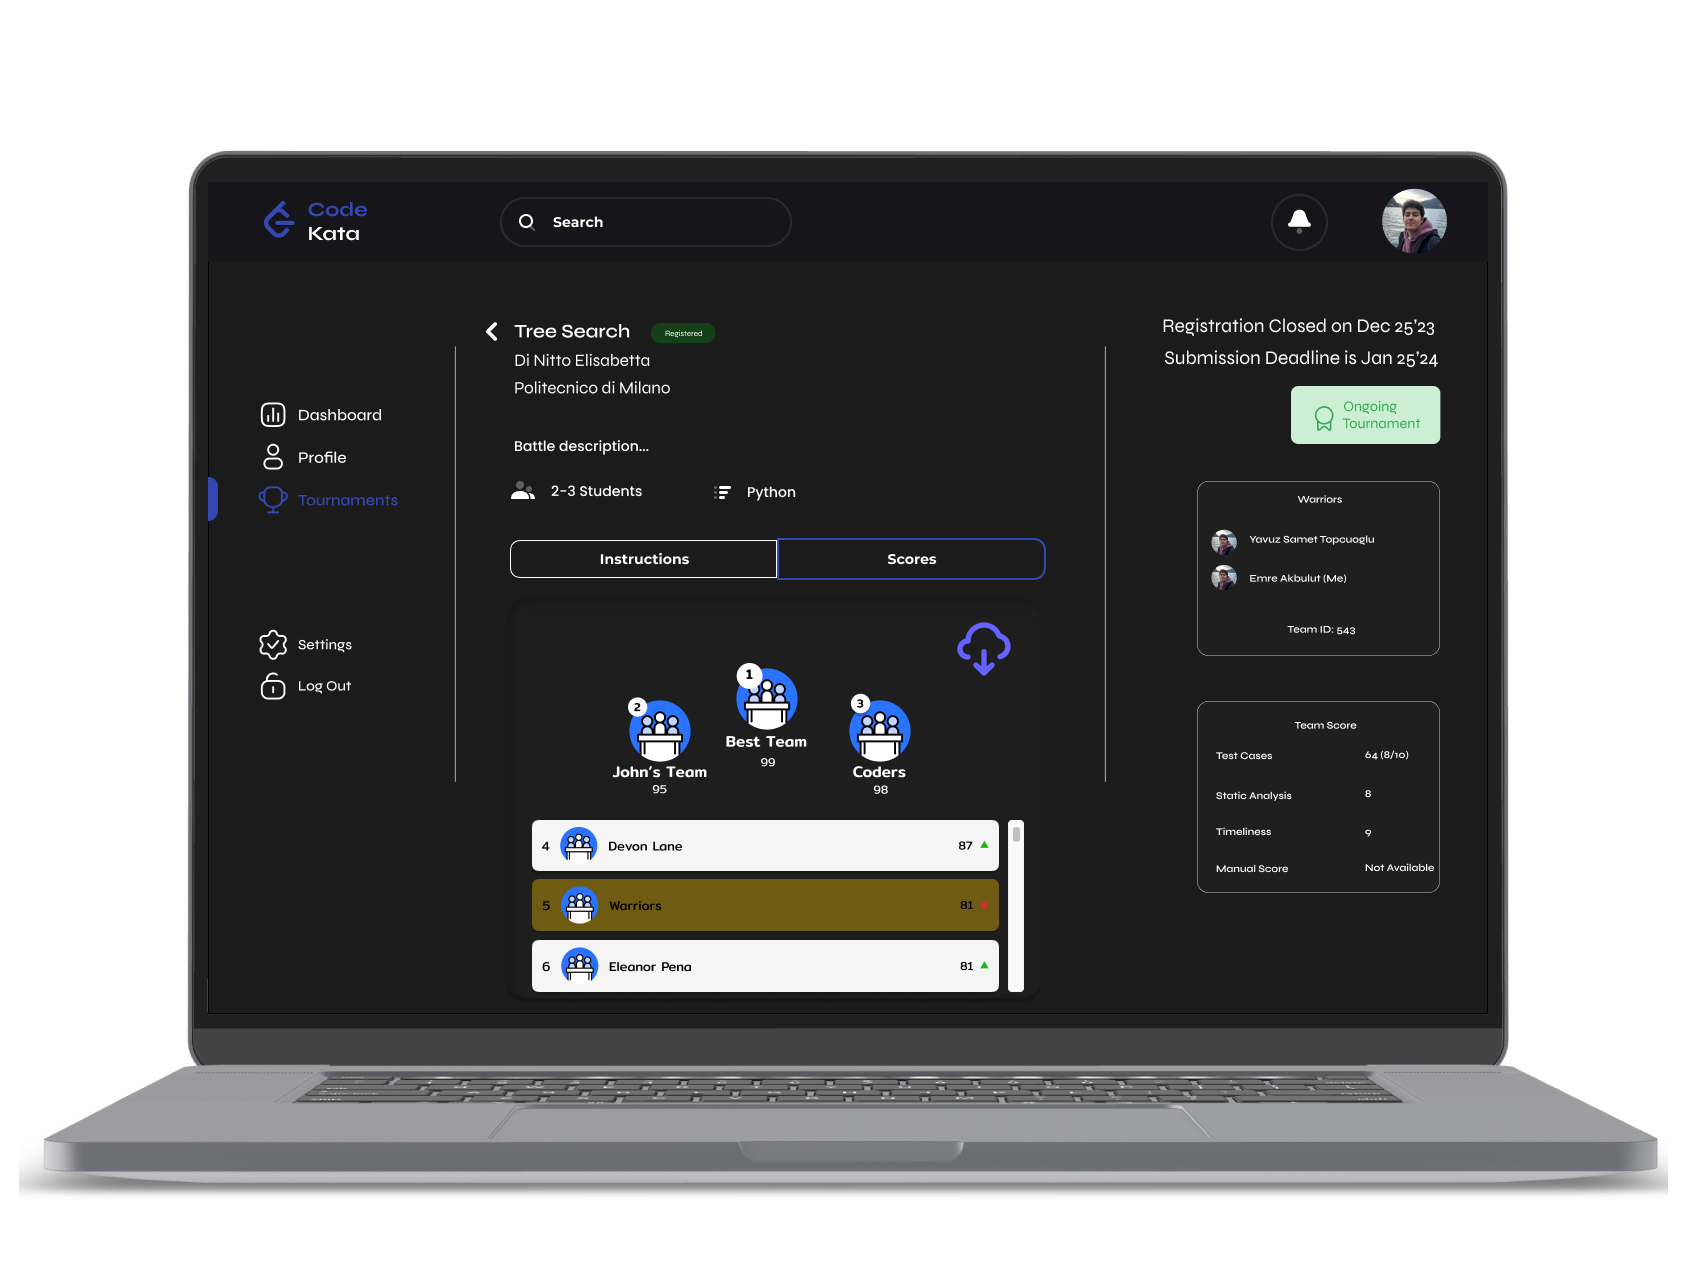
\includegraphics[scale=0.13]{Images/ui-ux/student_battle_4.png}
      (g) $UI_{7}$  Battle Screen for Student
\end{center}

\begin{center}
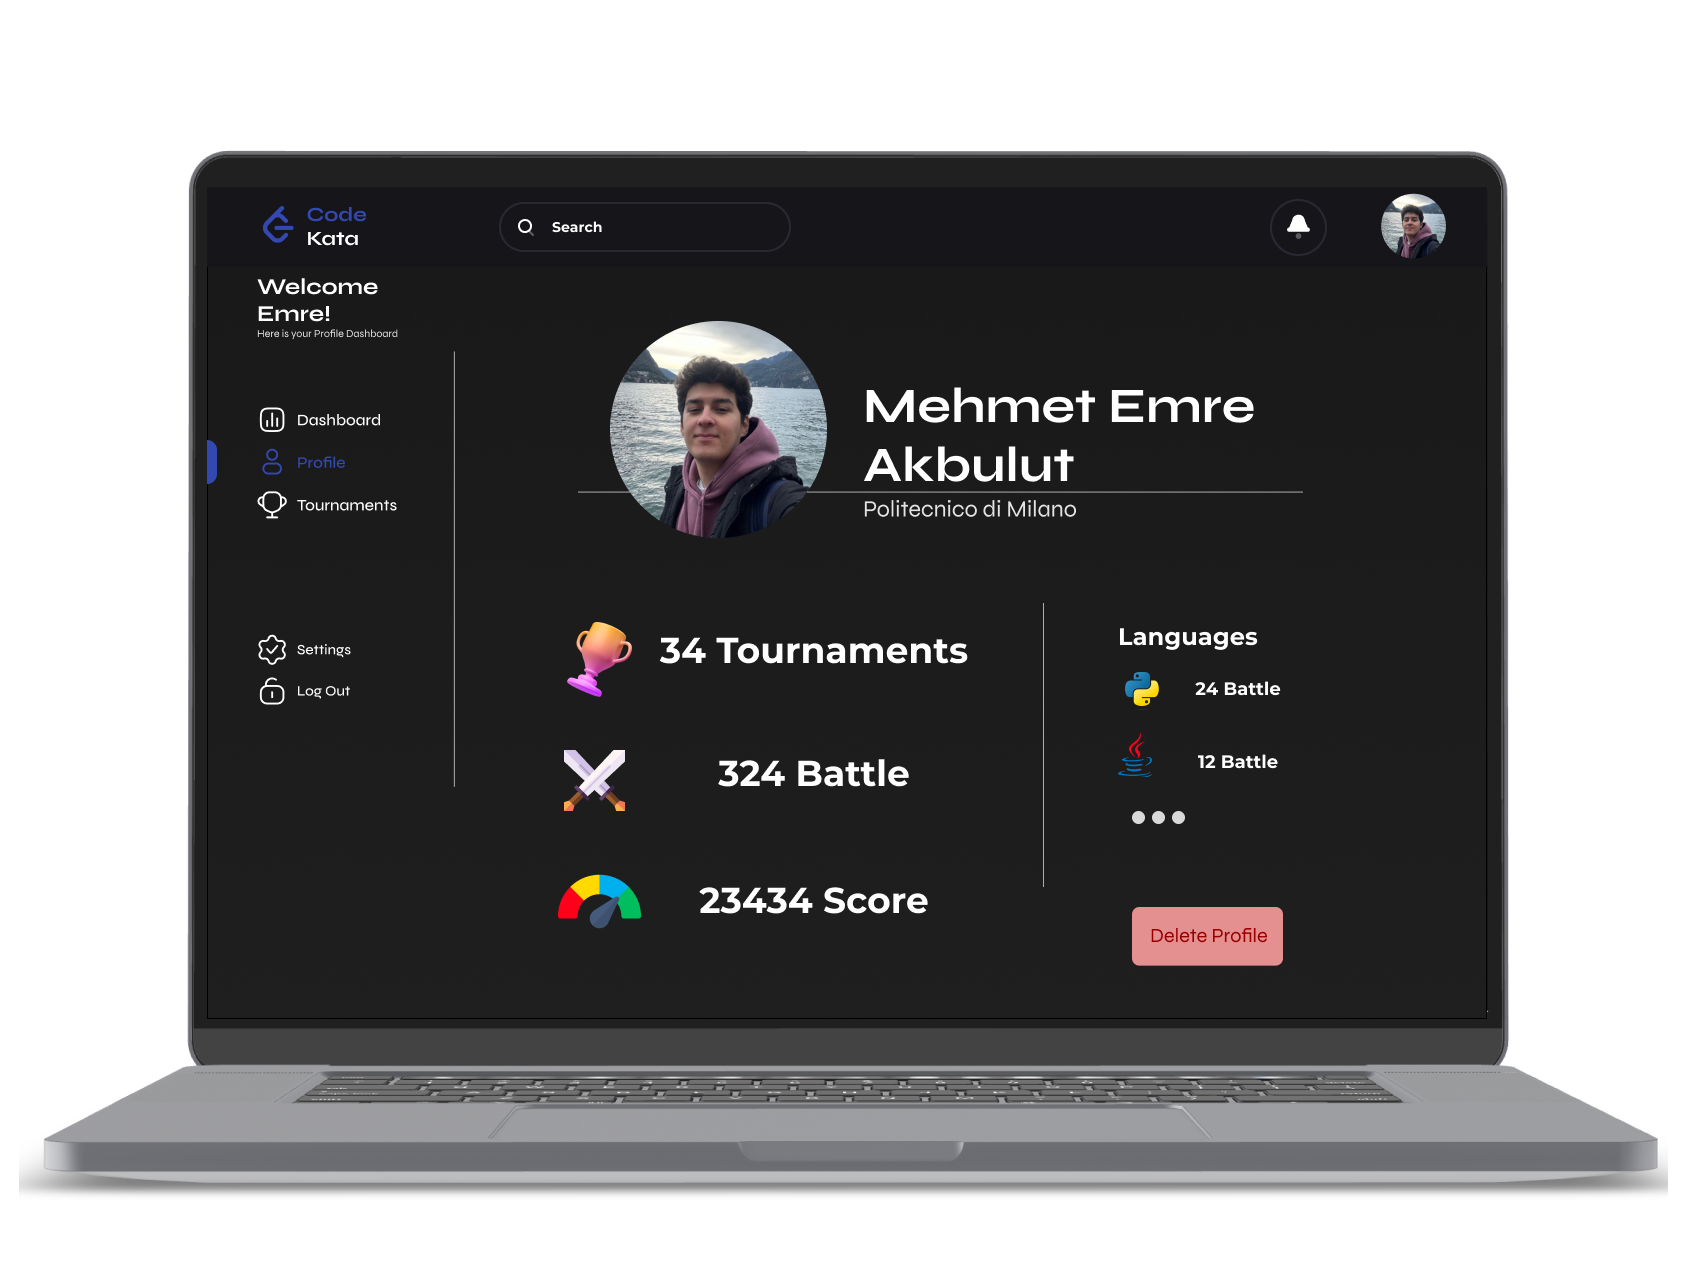
\includegraphics[scale=0.13]{Images/ui-ux/student_profile.png}
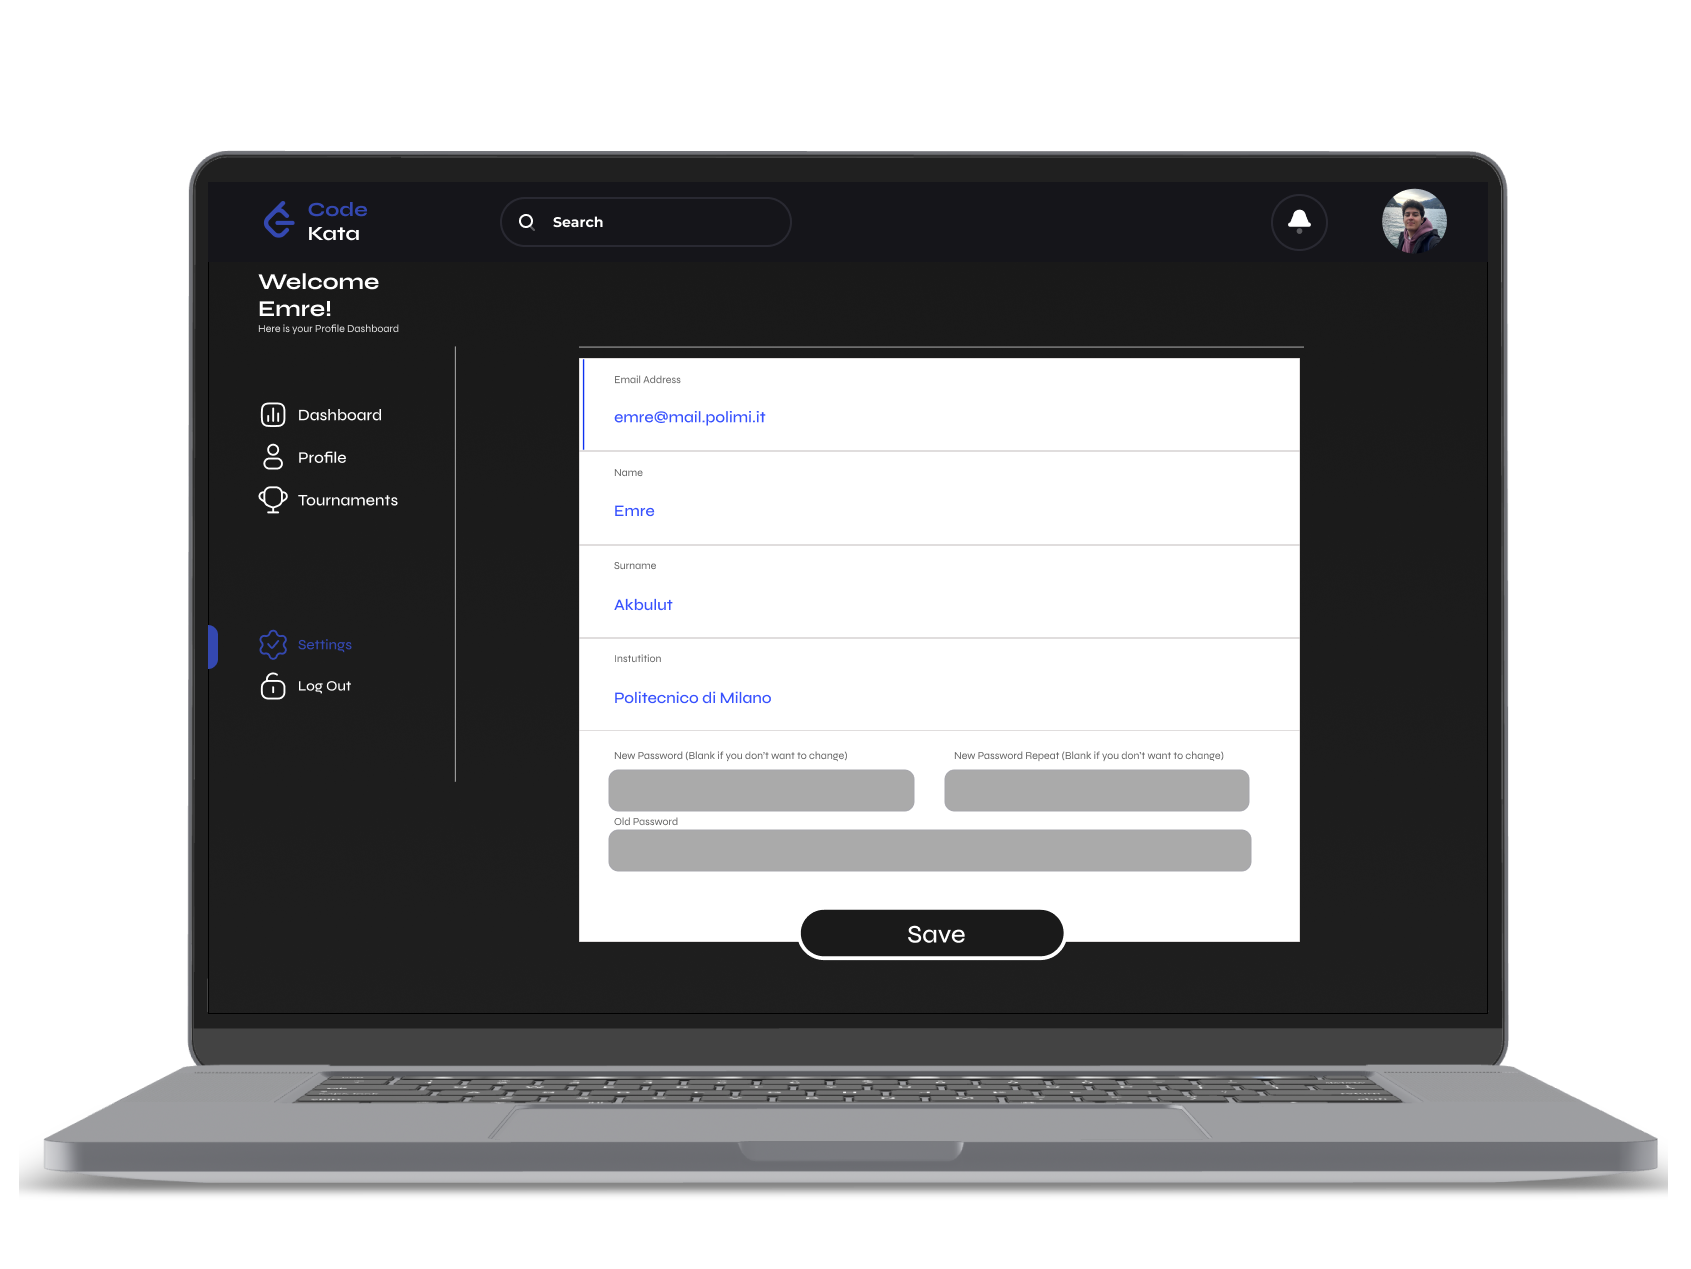
\includegraphics[scale=0.13]{Images/ui-ux/student_settings.png}
        (h) $UI_{8}$  Profile and Settings for Student
\end{center}
\newpage
\begin{center}
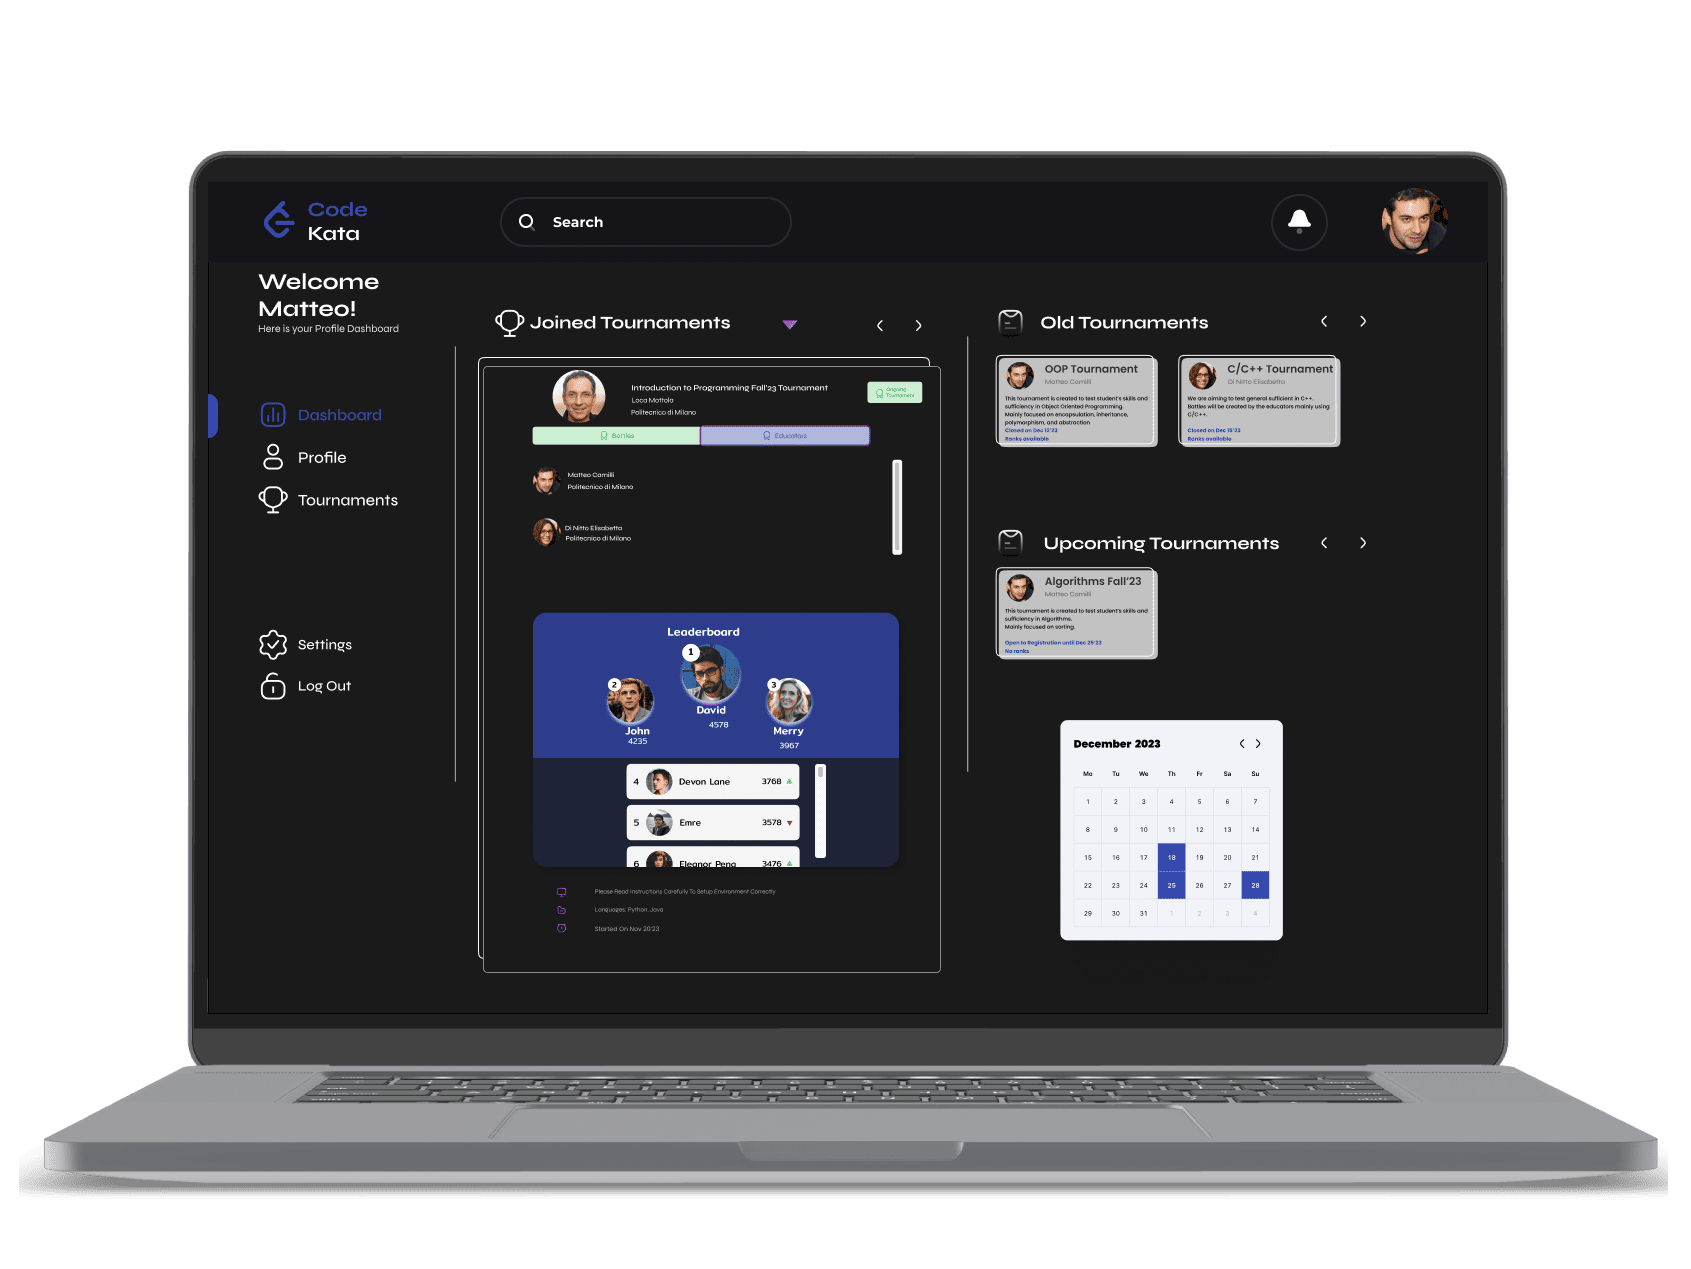
\includegraphics[scale=0.13]{Images/ui-ux/educator_dashboard_1.png}
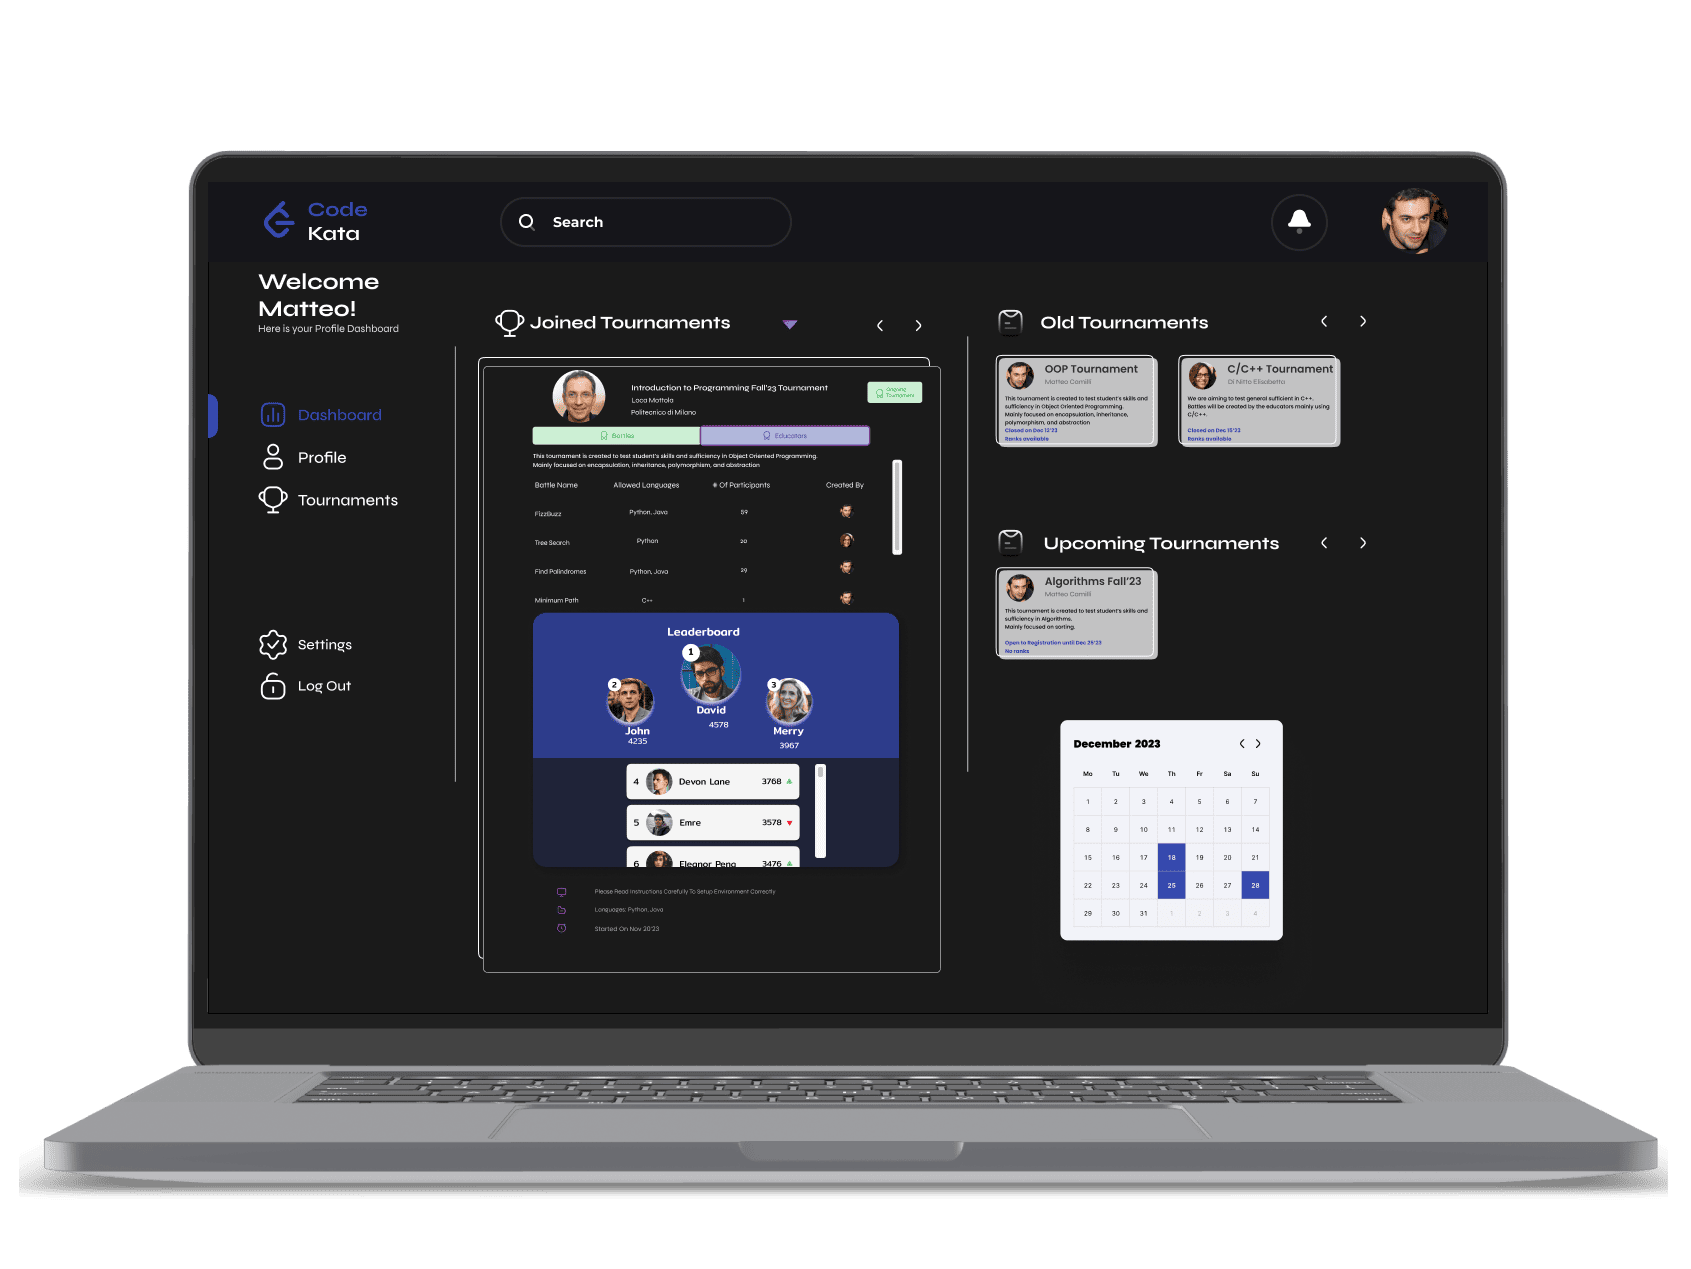
\includegraphics[scale=0.13]{Images/ui-ux/educator_dashboard_2.png}
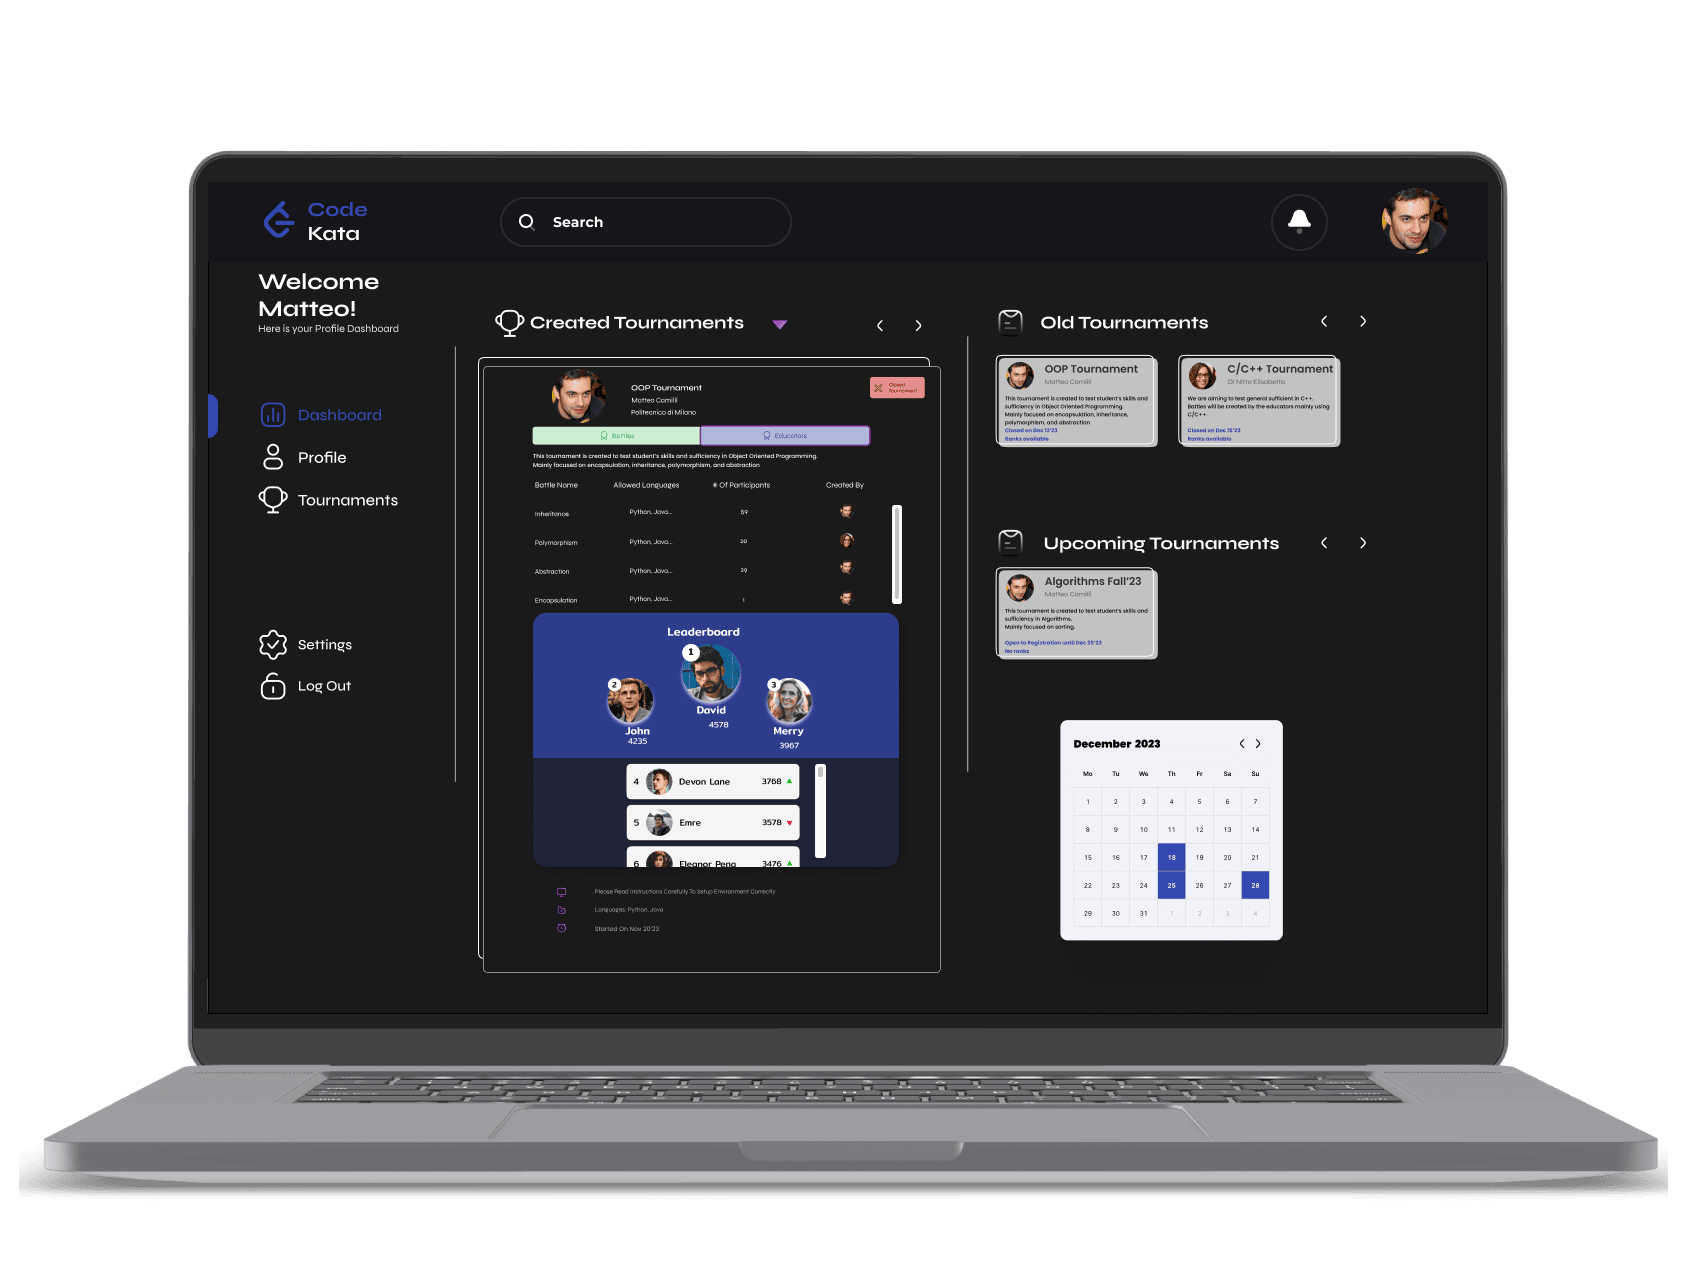
\includegraphics[scale=0.13]{Images/ui-ux/educator_dashboard_3.png}
\\ (i) $UI_{9}$  Educator Dashboard
\end{center}
\begin{center}
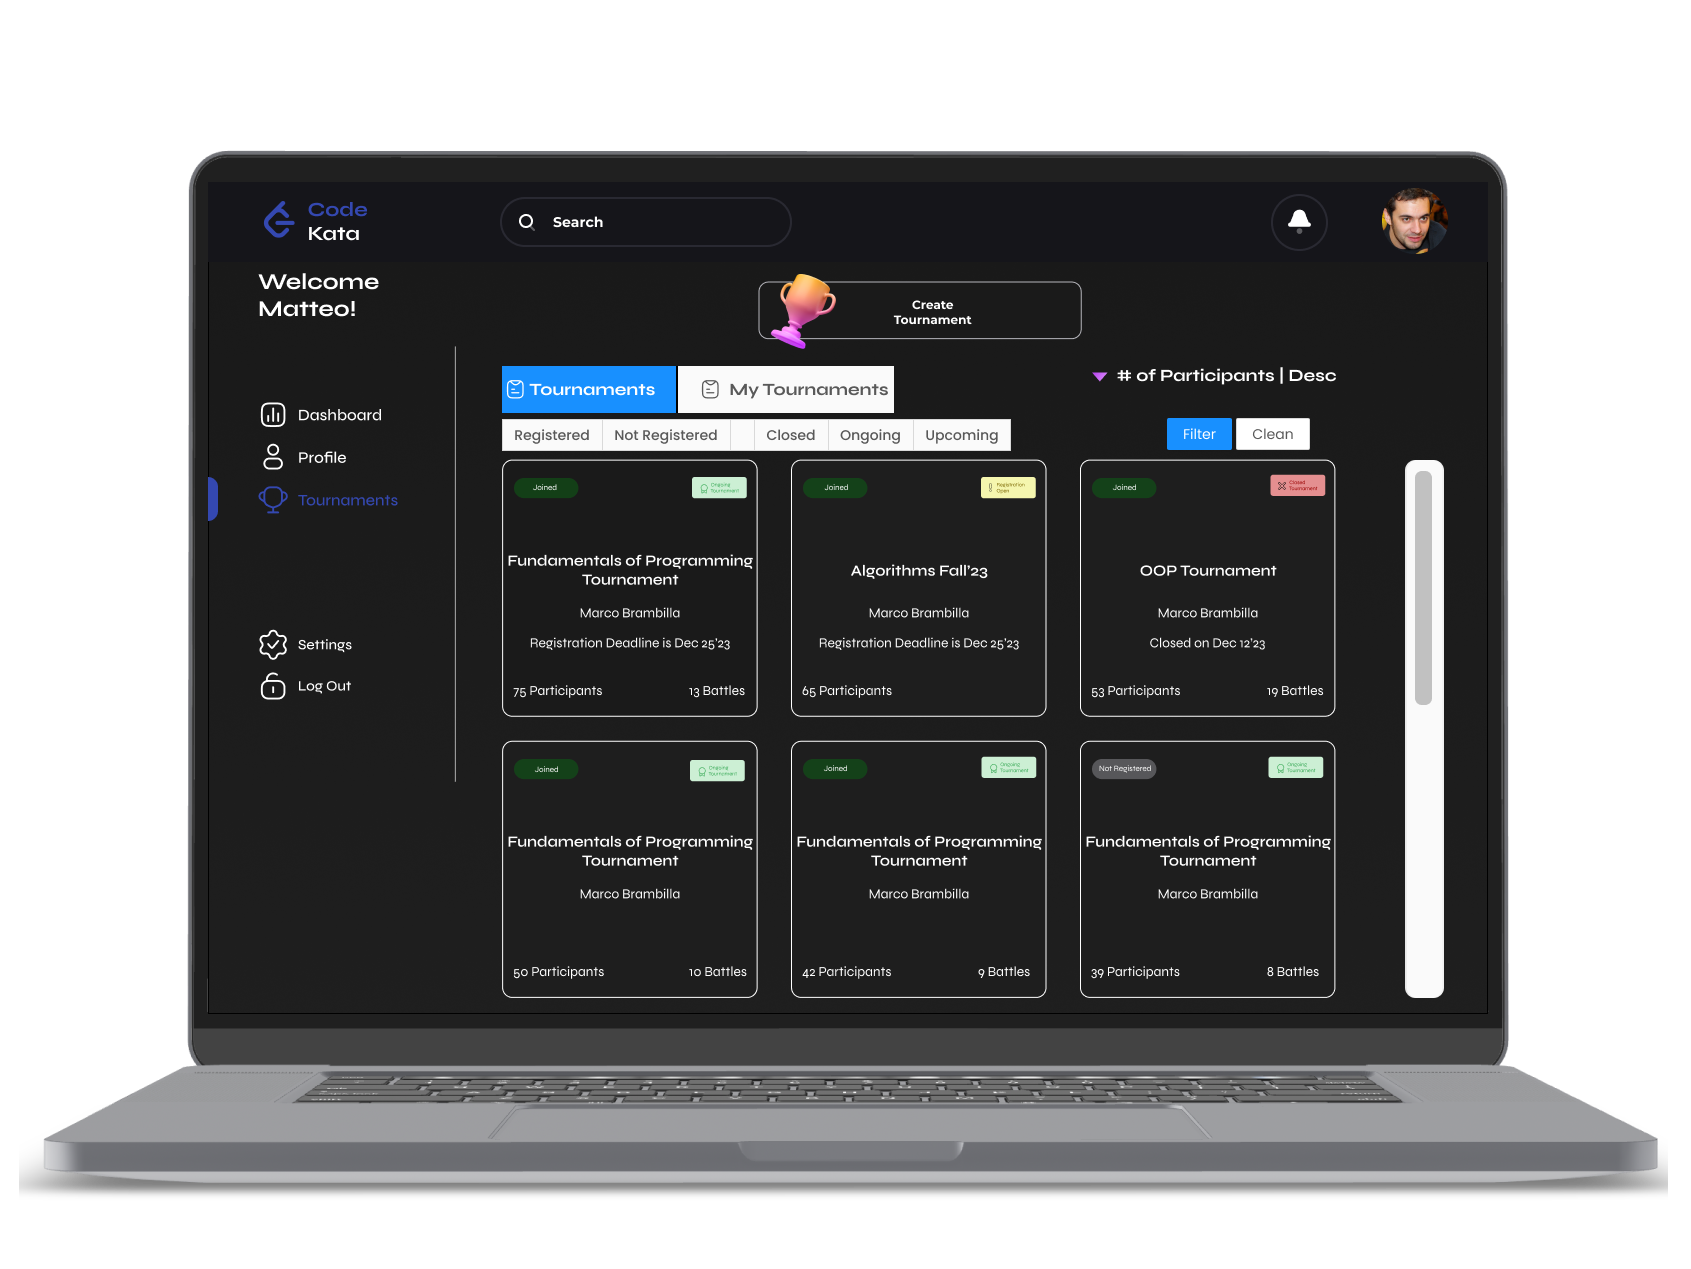
\includegraphics[scale=0.13]{Images/ui-ux/educator_tournaments_1.png}
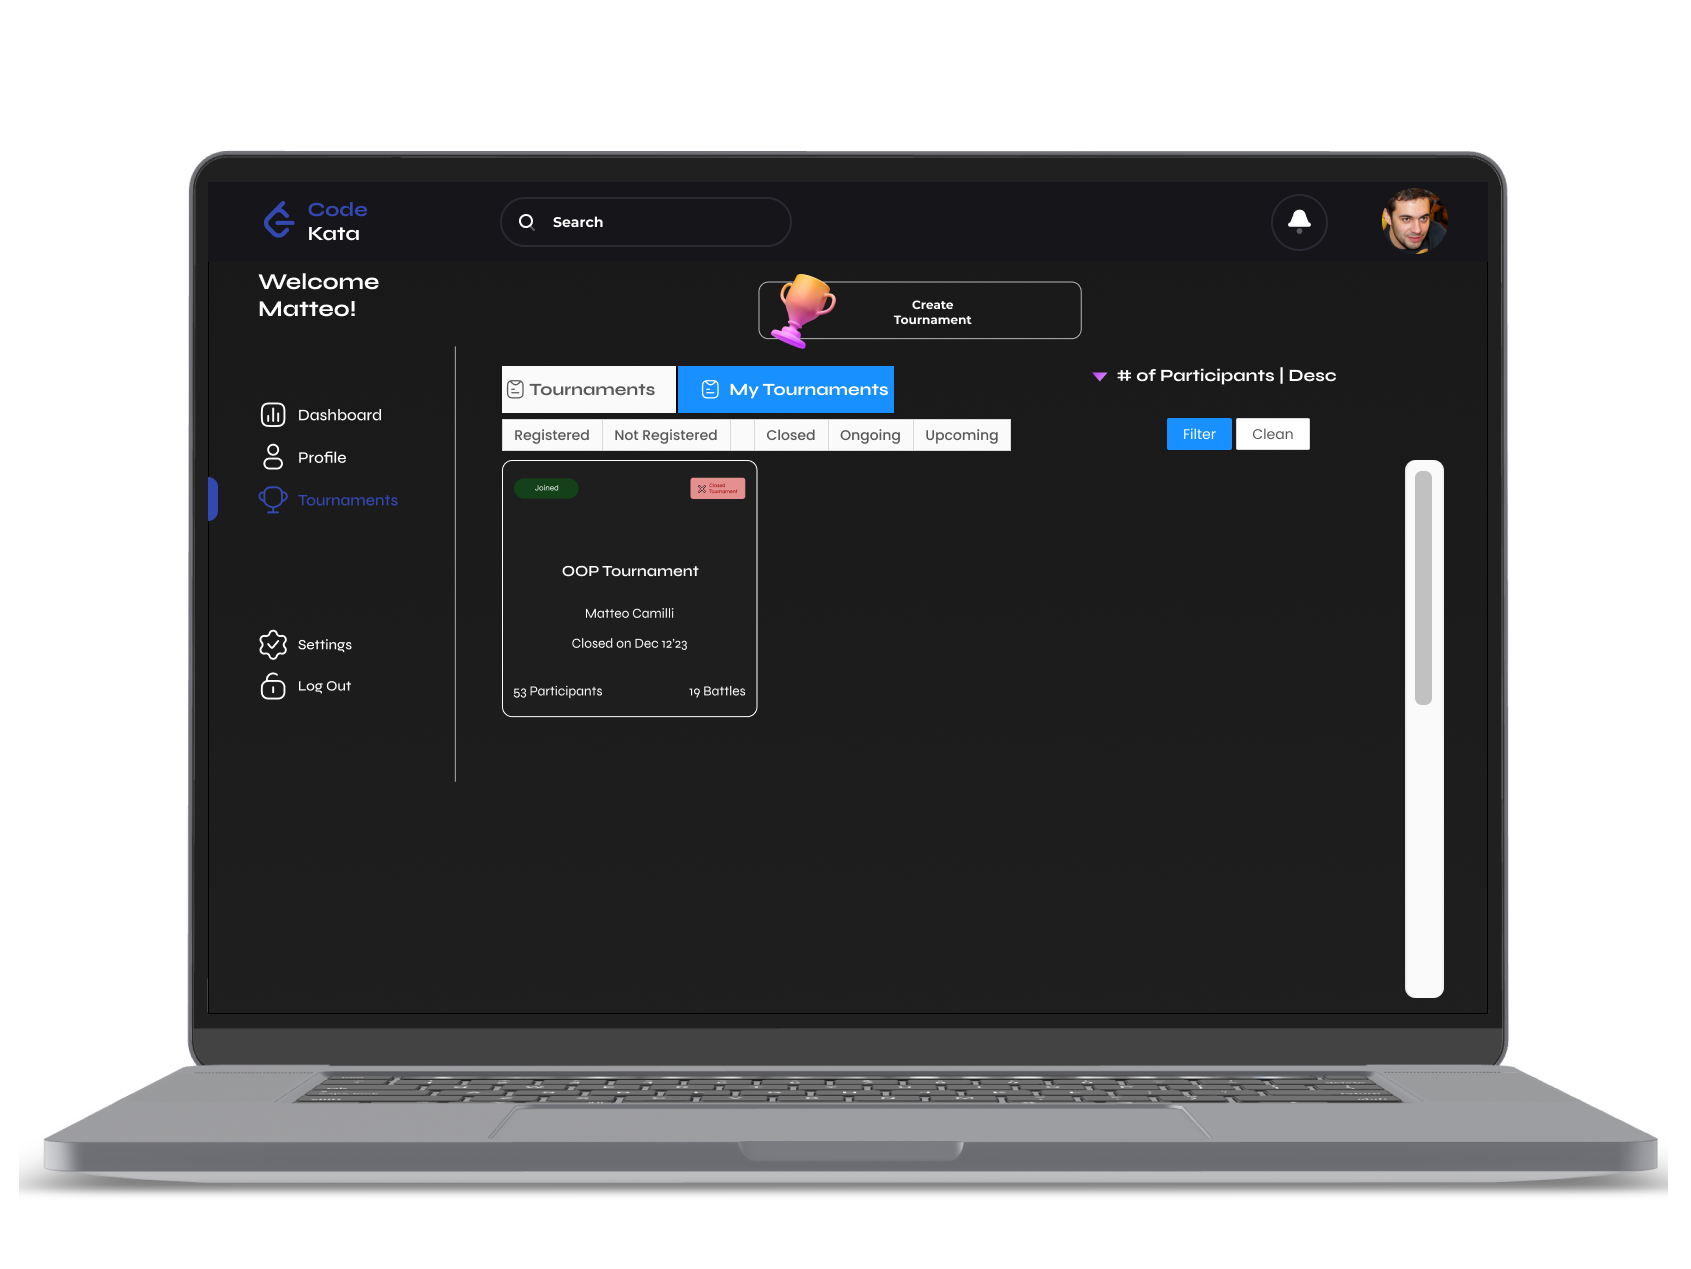
\includegraphics[scale=0.13]{Images/ui-ux/educator_tournaments_2.png}
        (j) $UI_{10}$  Educator Tournaments
\end{center}
\begin{center}
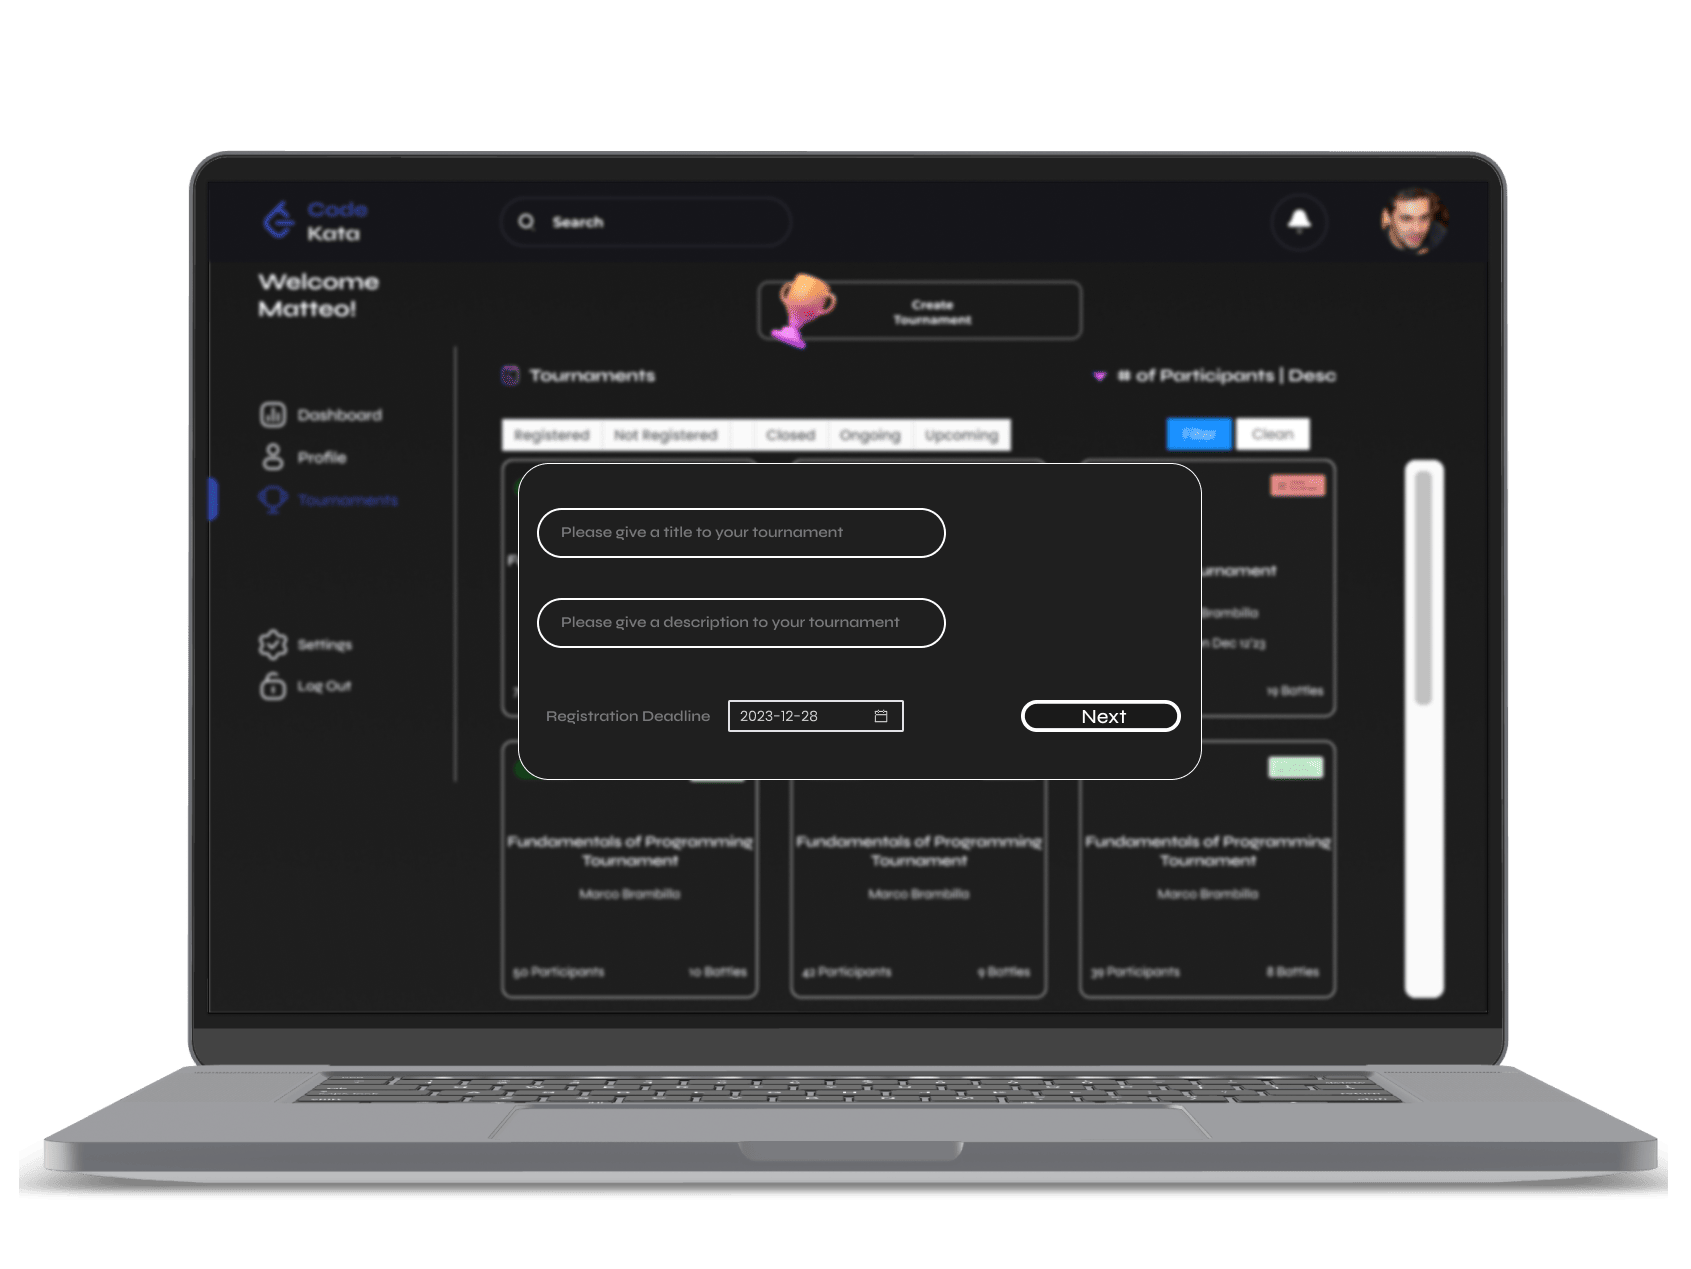
\includegraphics[scale=0.13]{Images/ui-ux/educator_create_tournament_1.png}
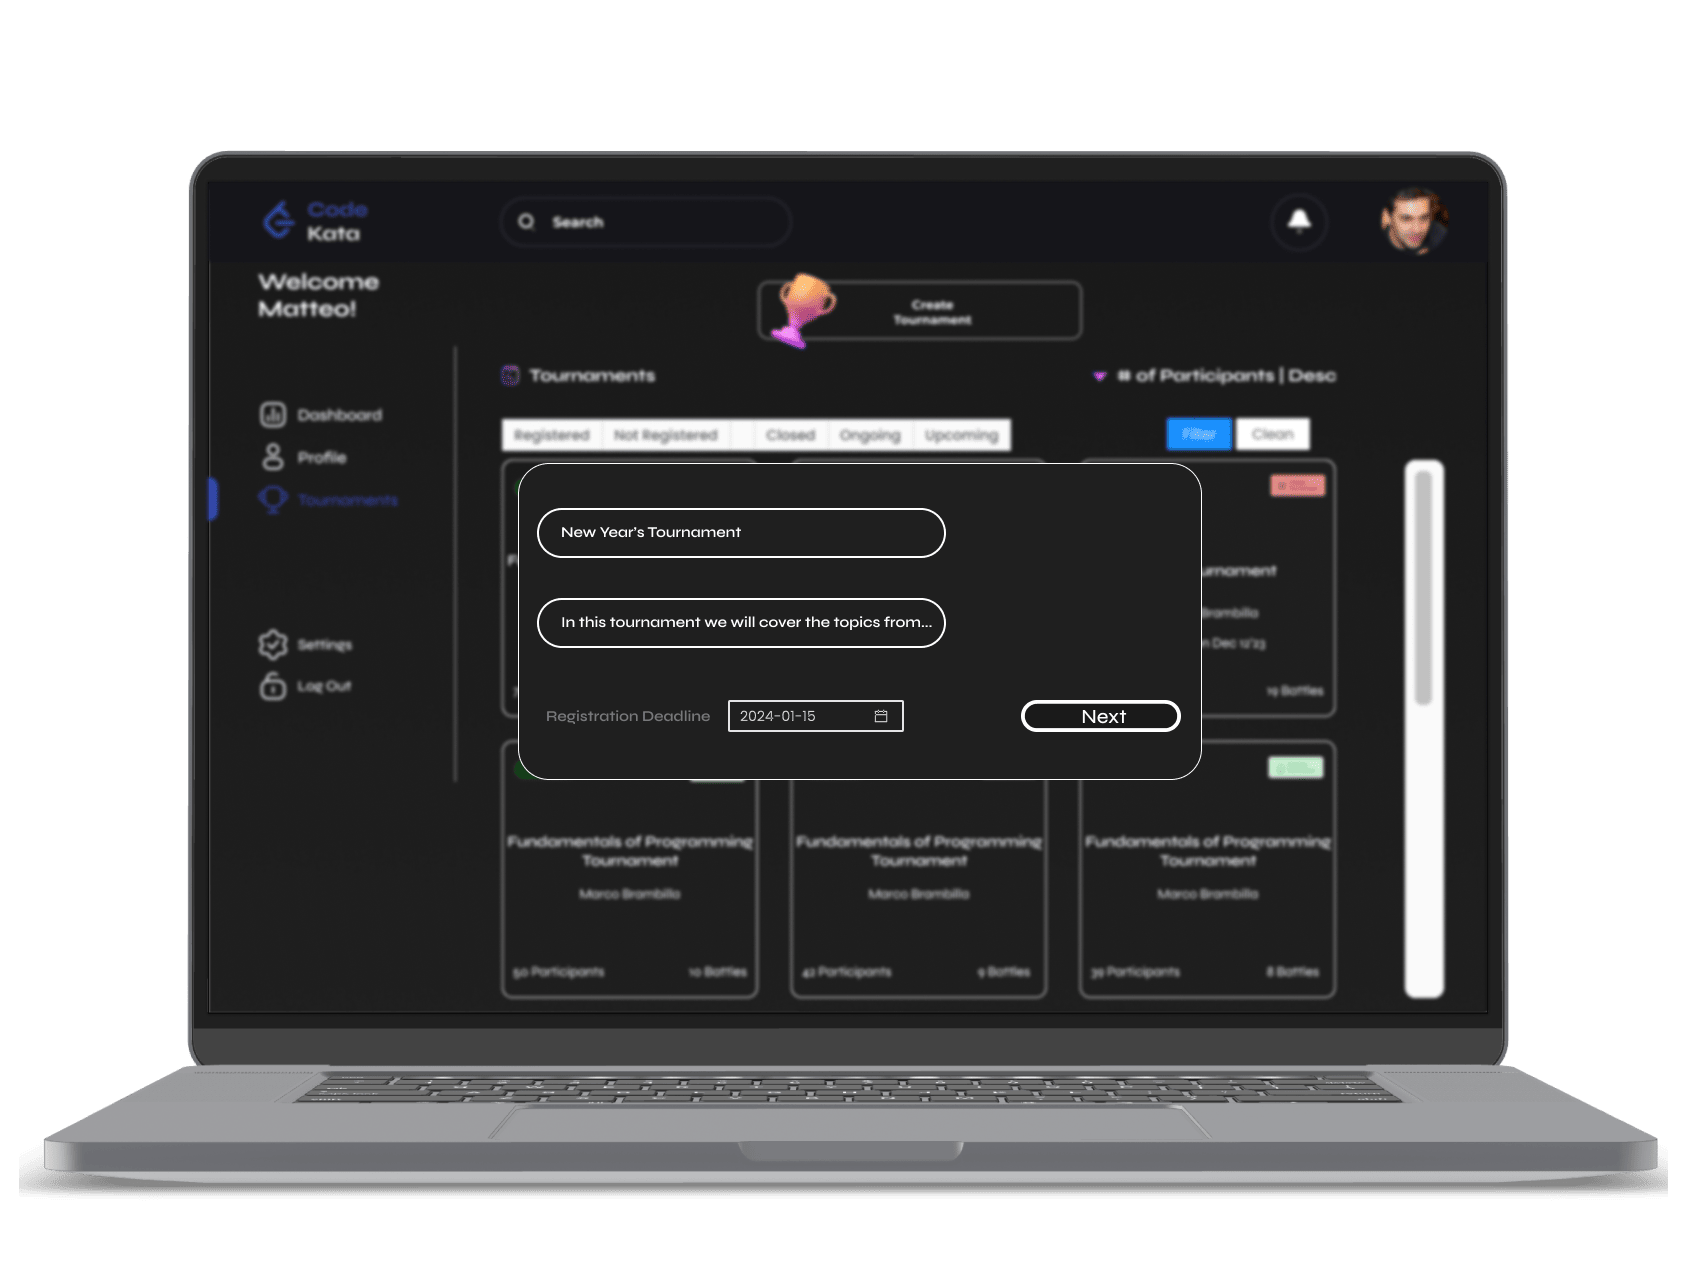
\includegraphics[scale=0.13]{Images/ui-ux/educator_create_tournament_2.png}
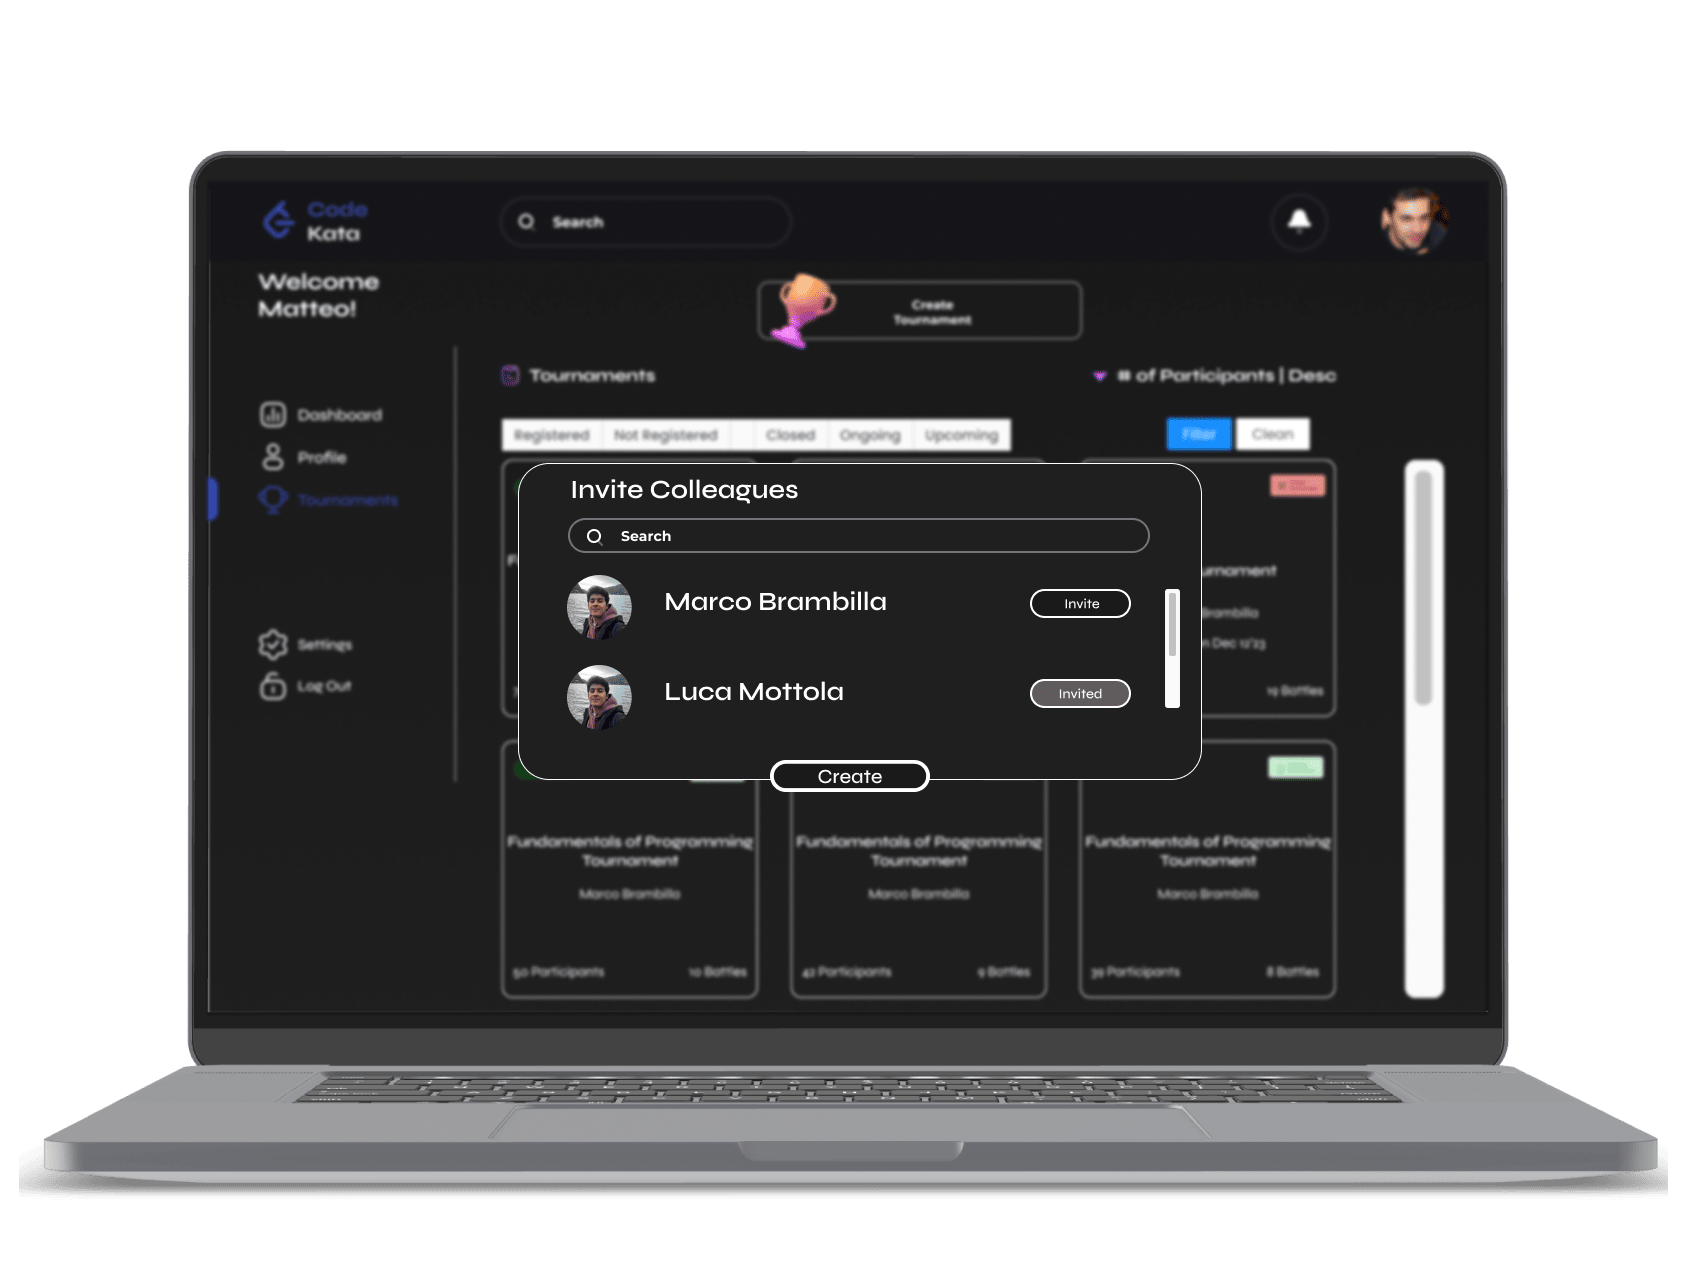
\includegraphics[scale=0.13]{Images/ui-ux/educator_create_tournament_3.png}
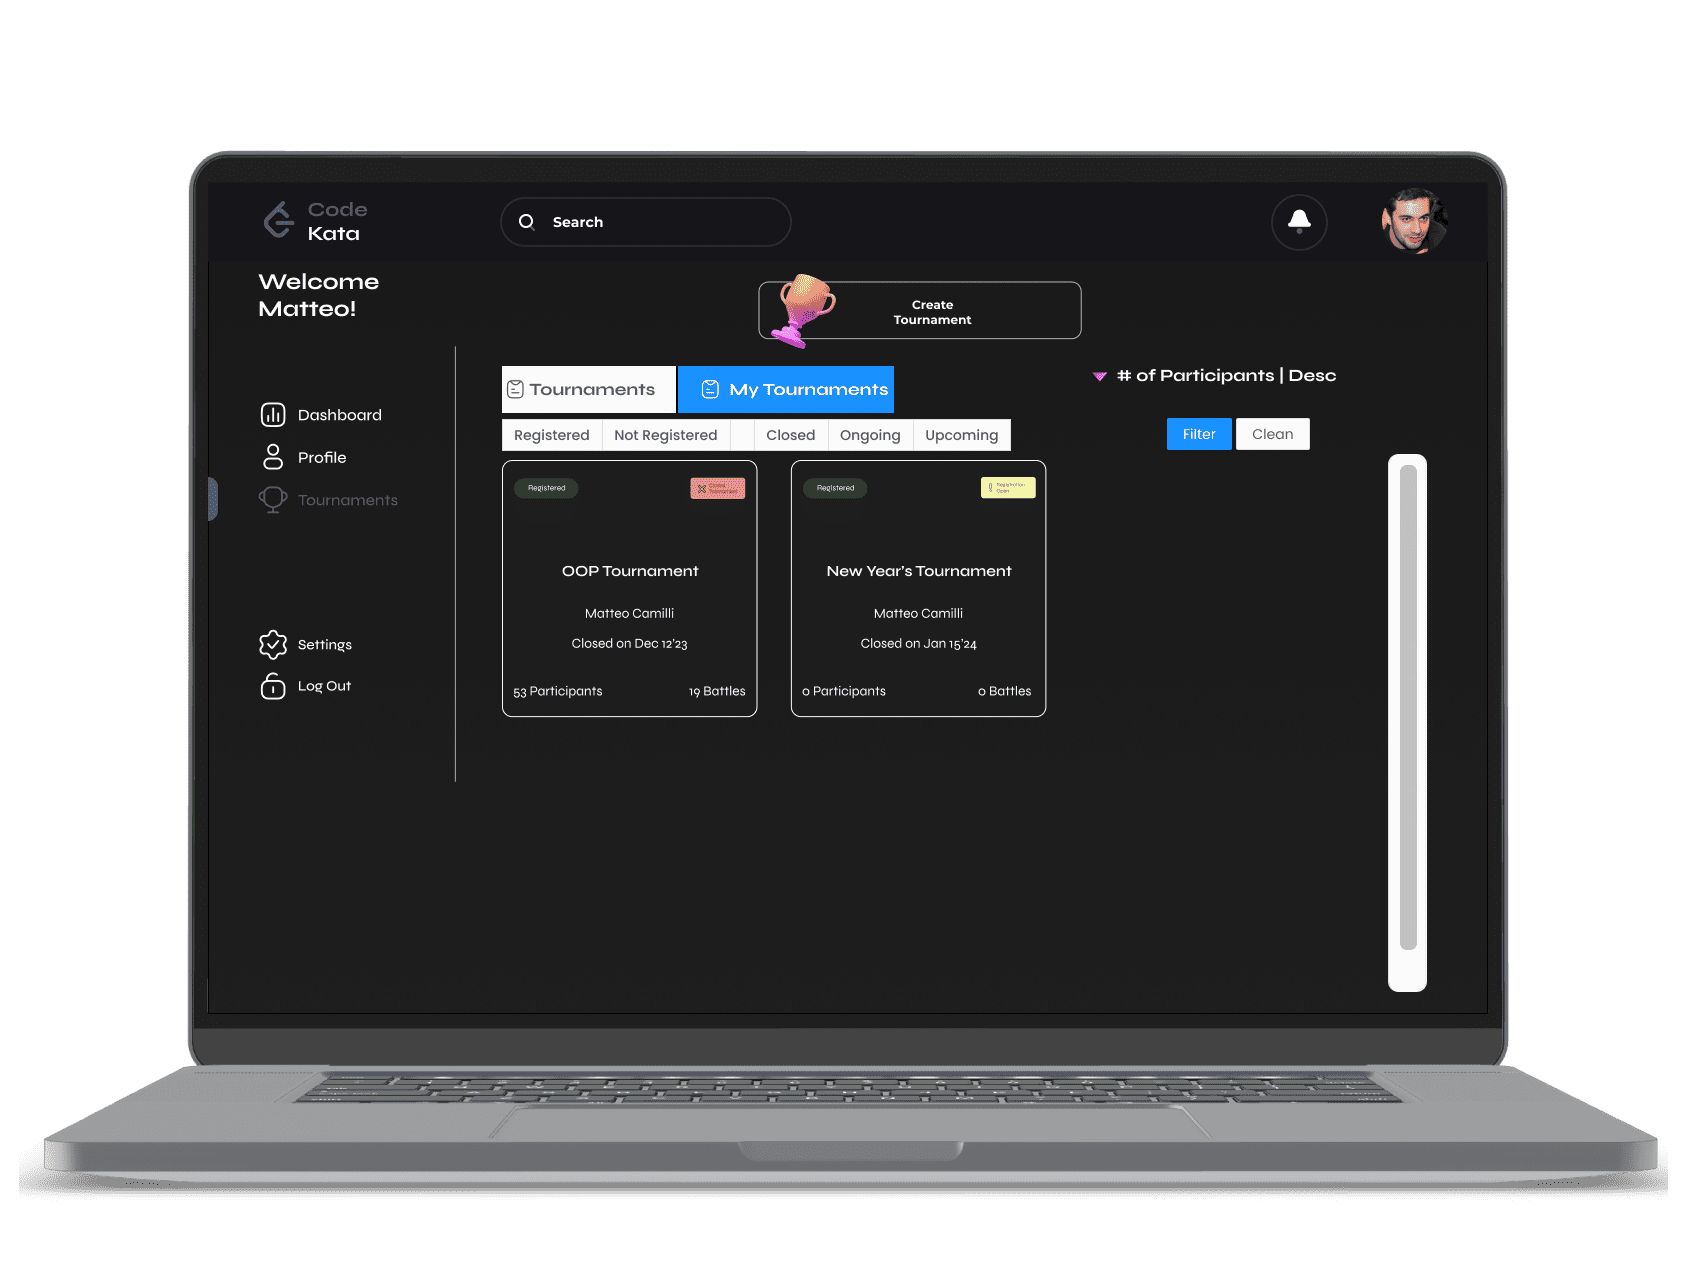
\includegraphics[scale=0.13]{Images/ui-ux/educator_create_tournament_4.png}
        (k) $UI_{11}$ Educator Creates Tournament
\end{center}
\newpage
\begin{center}
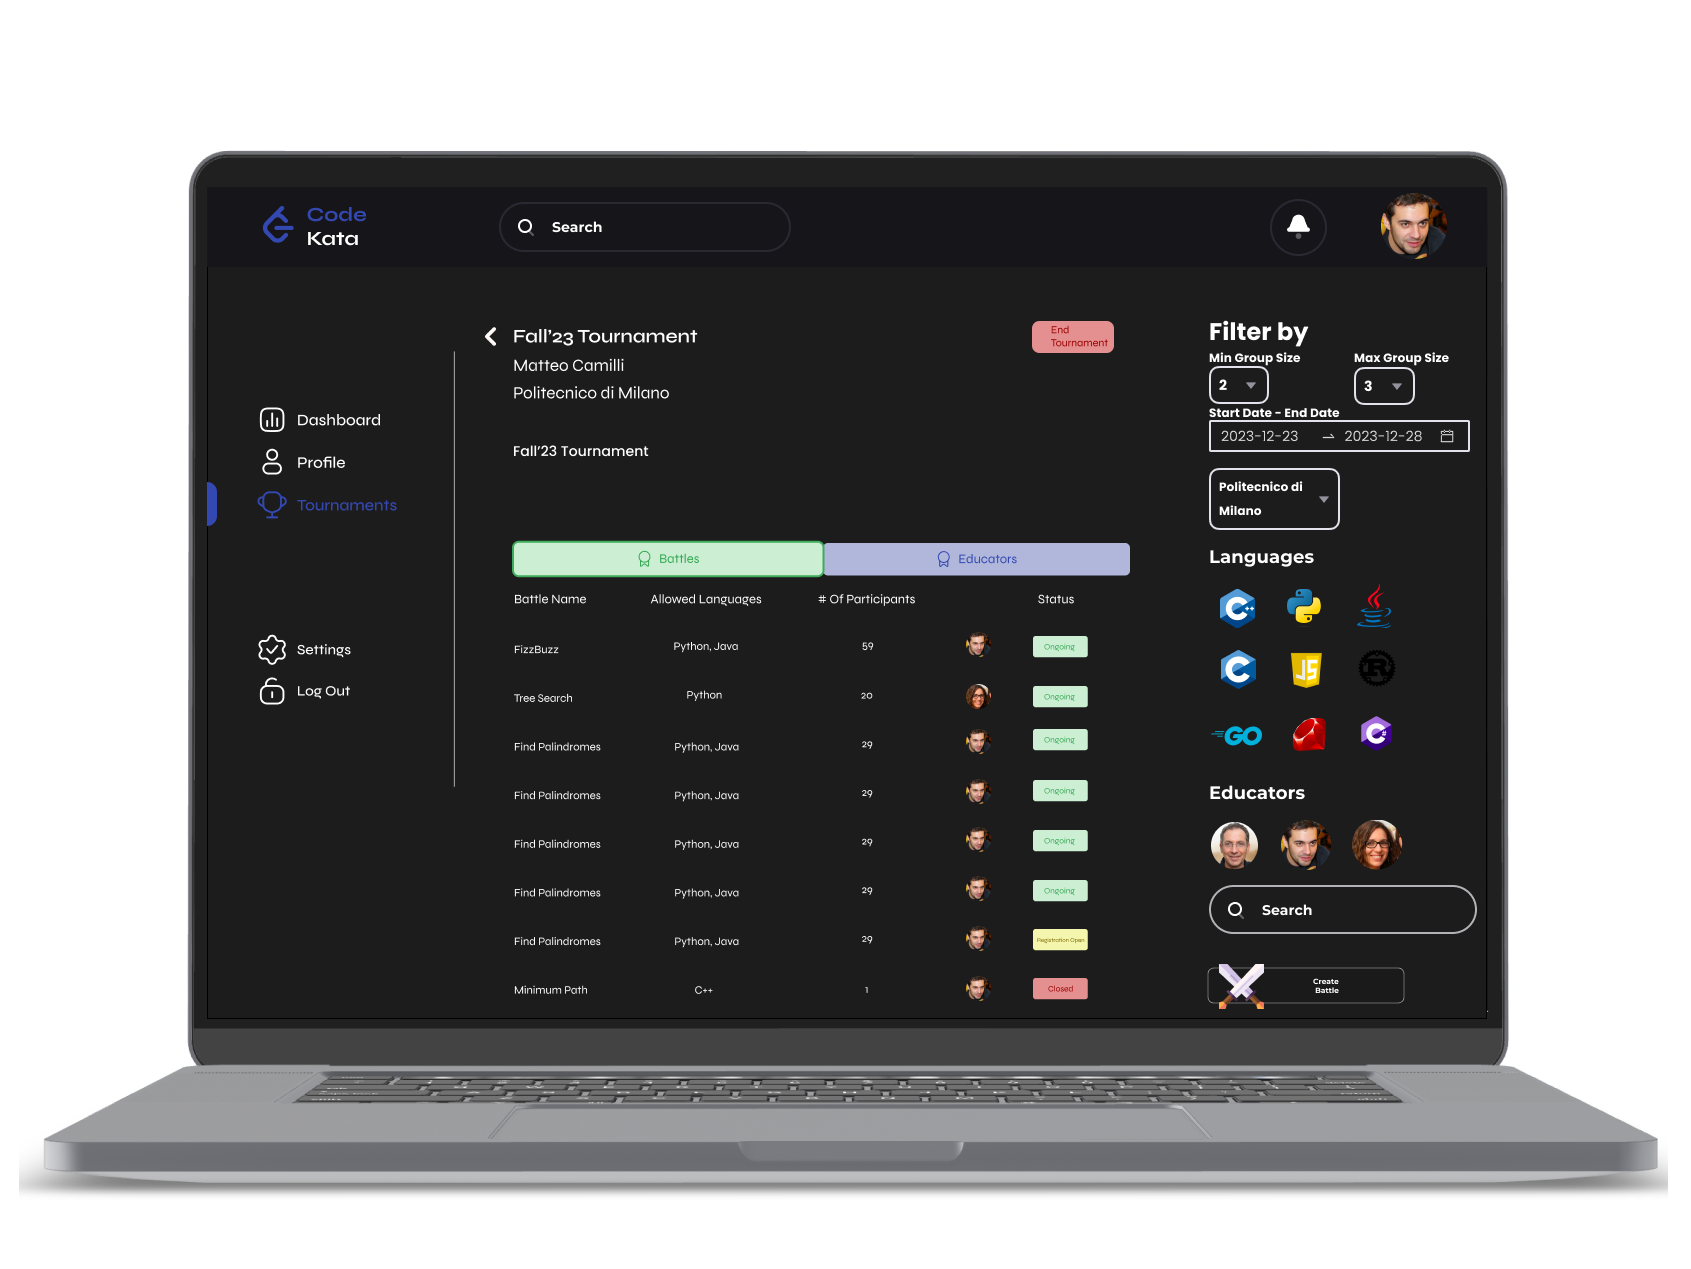
\includegraphics[scale=0.13]{Images/ui-ux/educator_creates_battle_1.png}
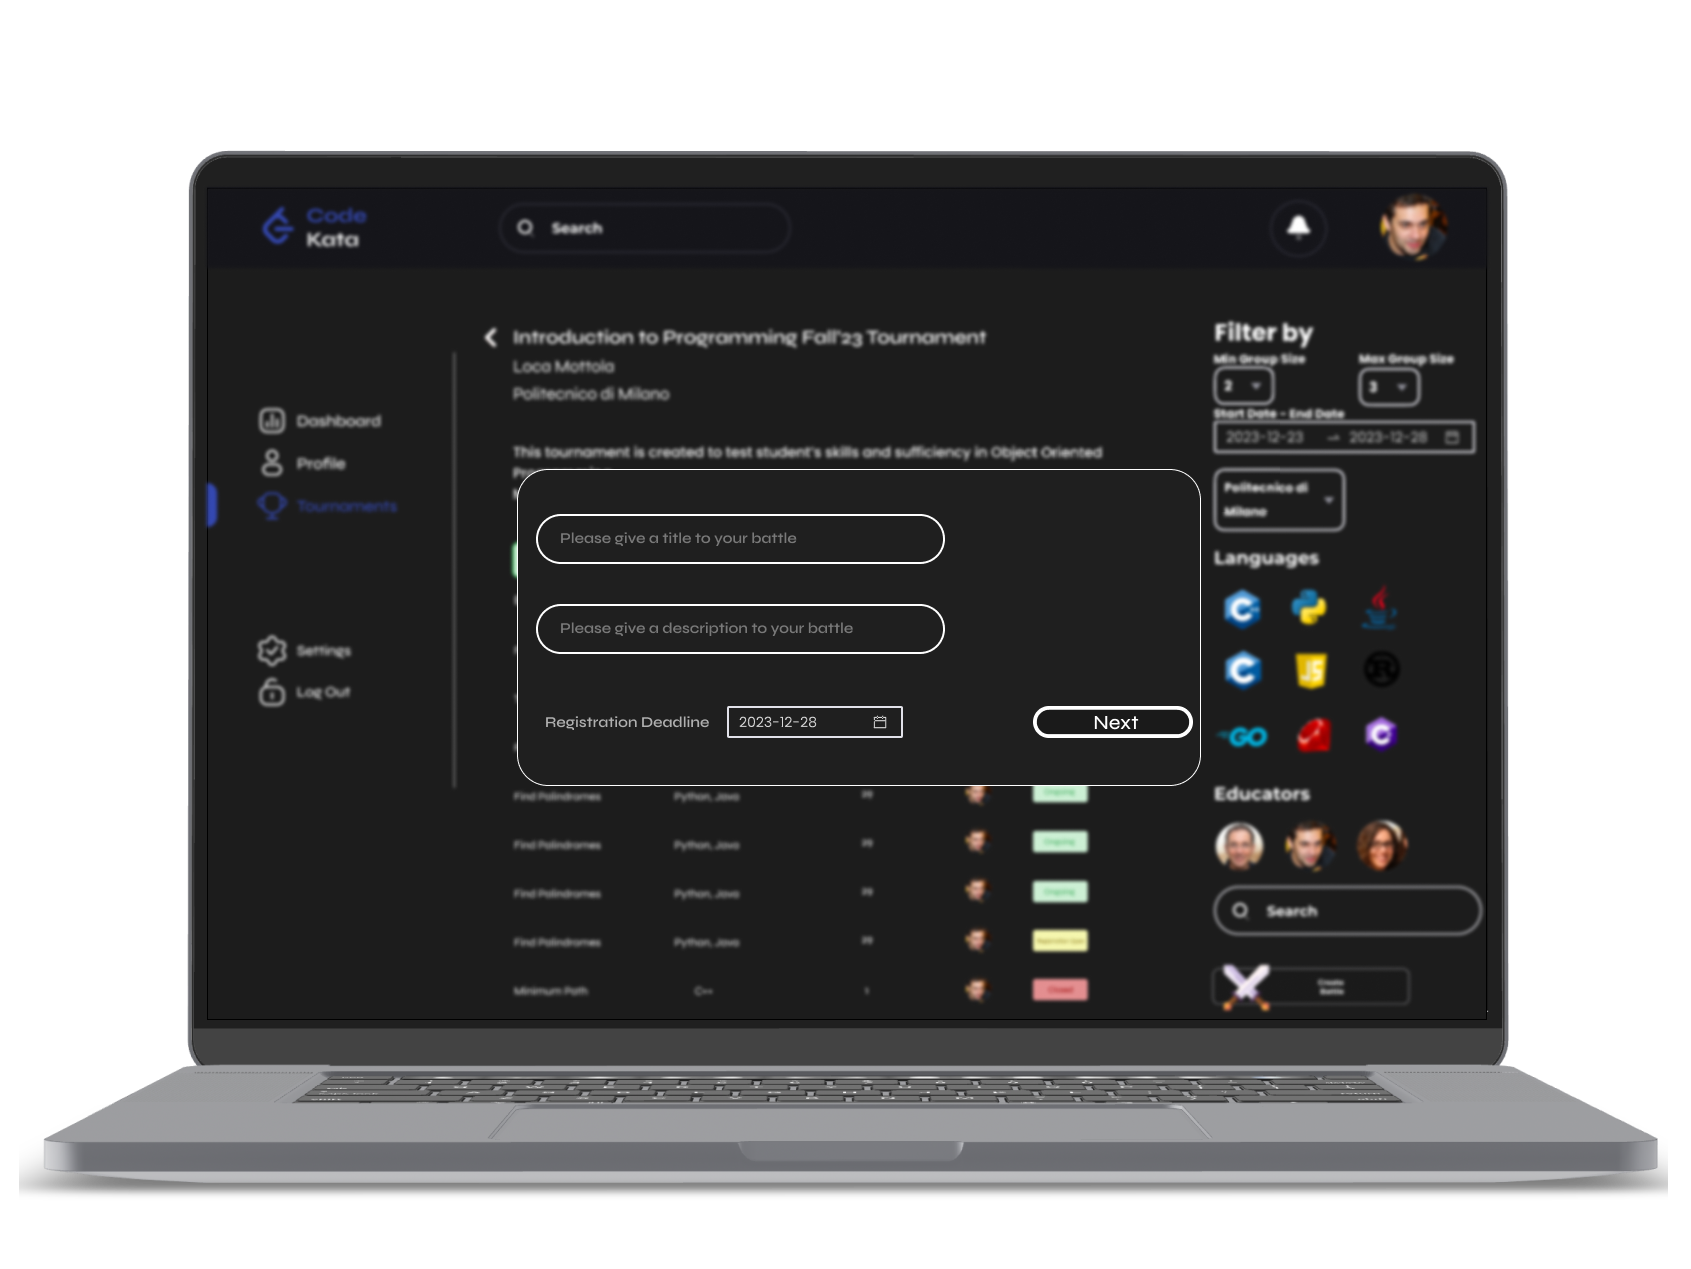
\includegraphics[scale=0.13]{Images/ui-ux/educator_creates_battle_2.png}
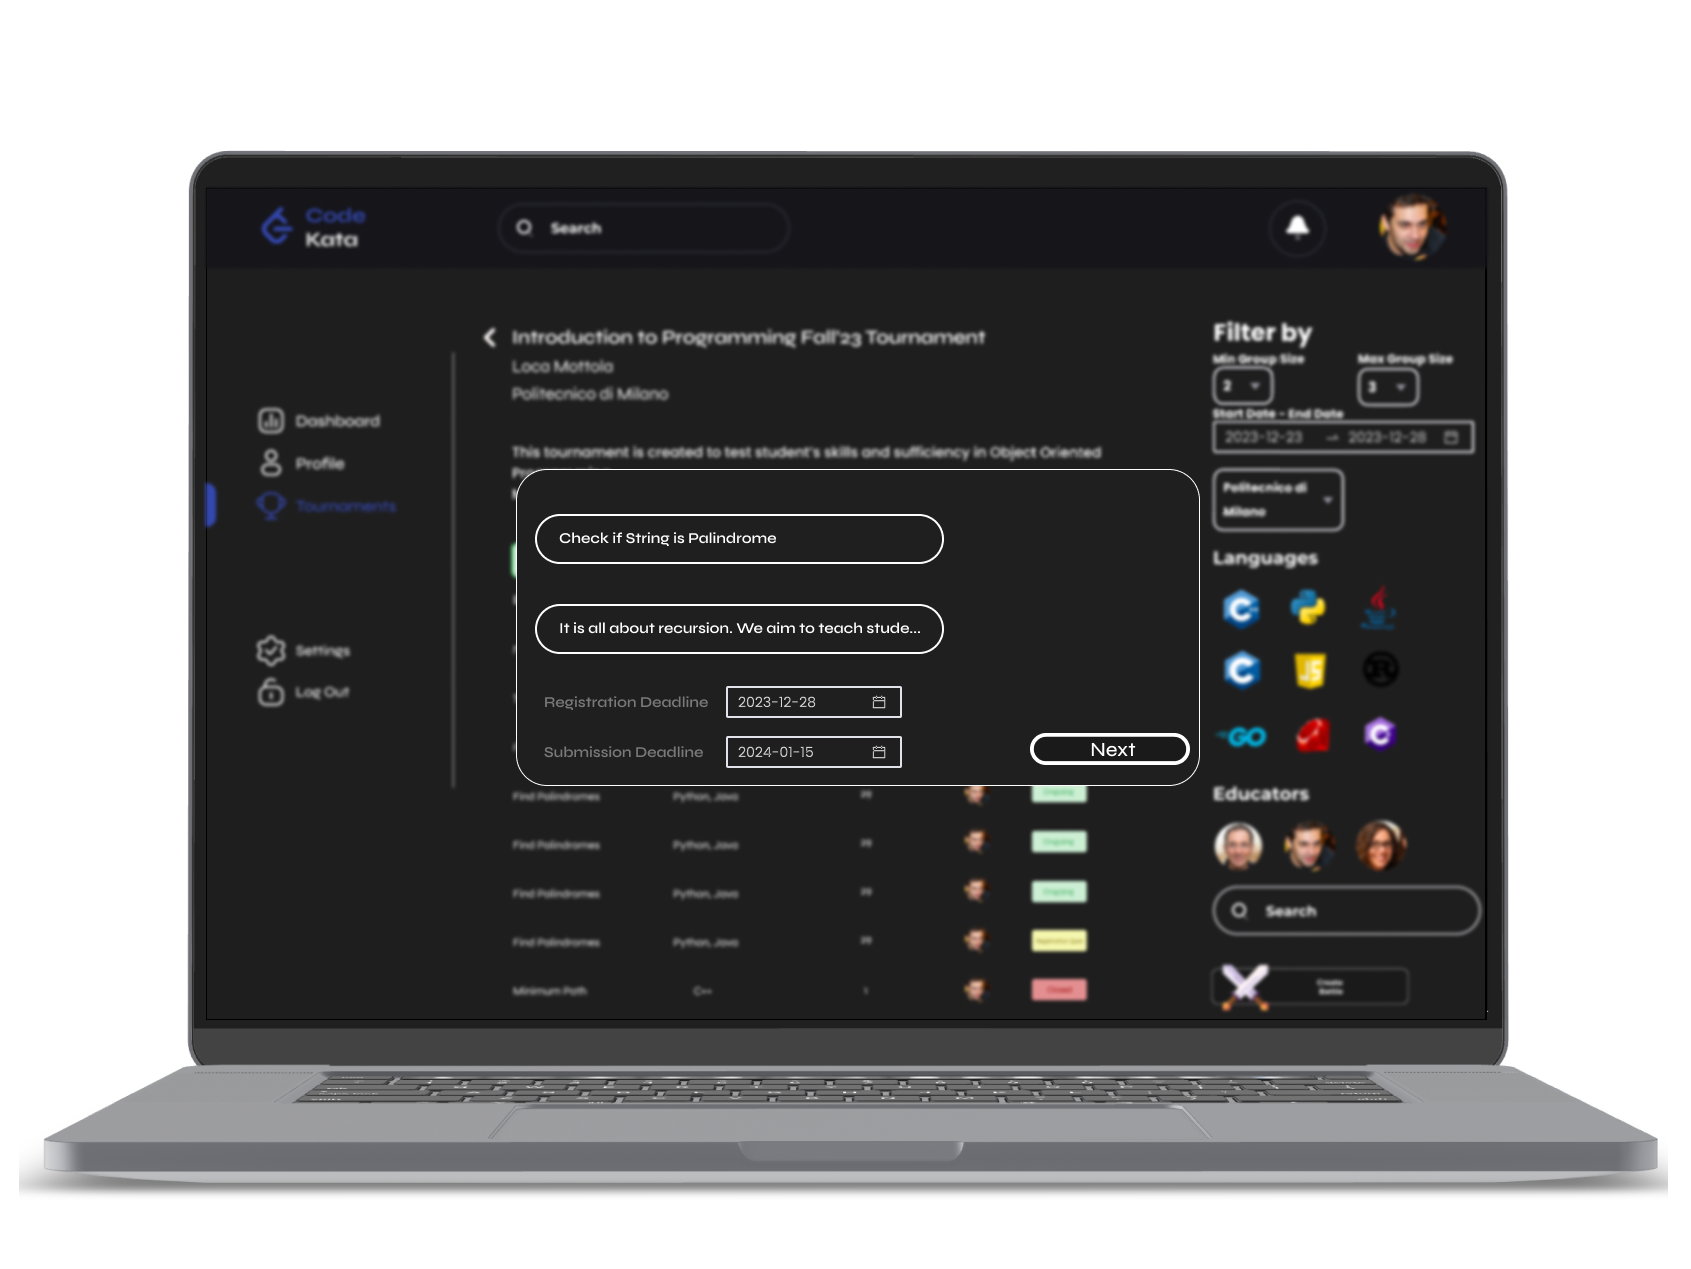
\includegraphics[scale=0.13]{Images/ui-ux/educator_creates_battle_3.png}
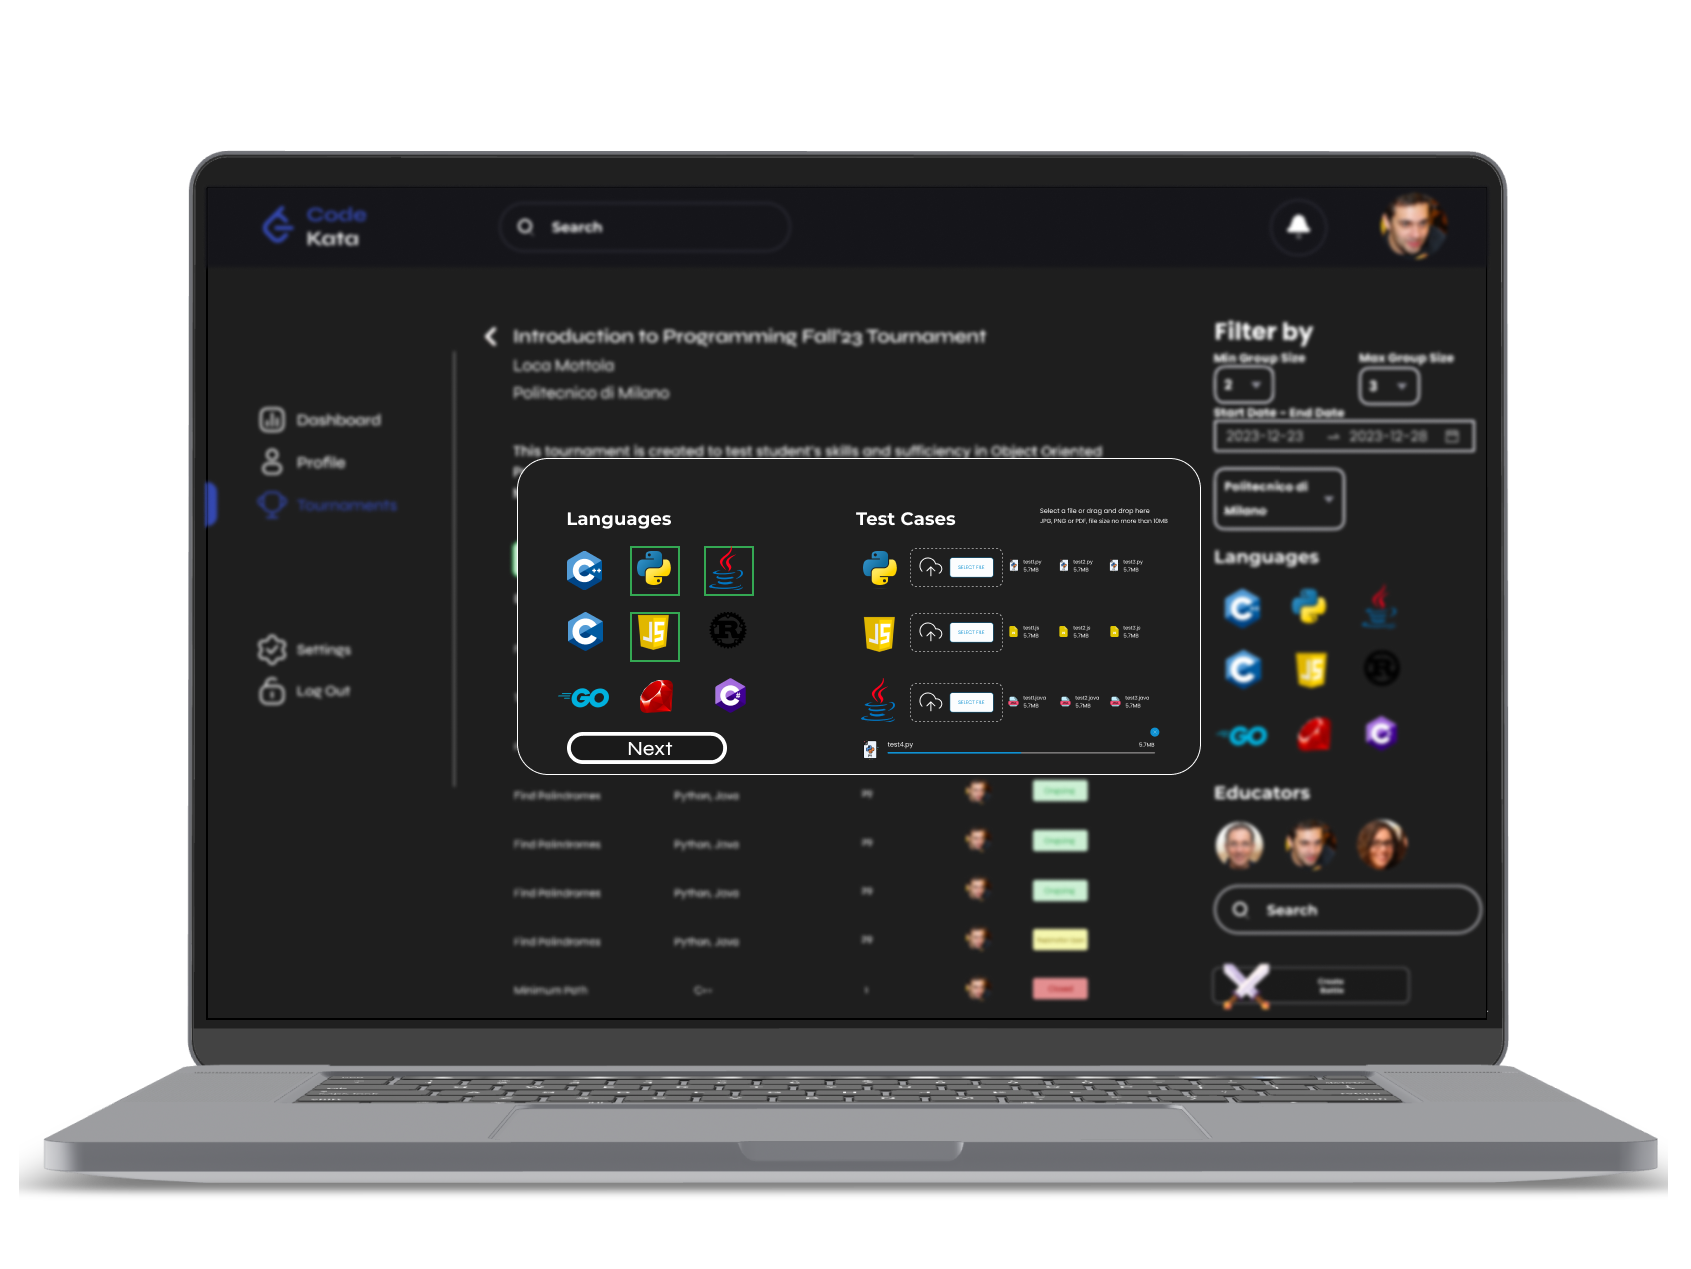
\includegraphics[scale=0.13]{Images/ui-ux/educator_creates_battle_4.png}
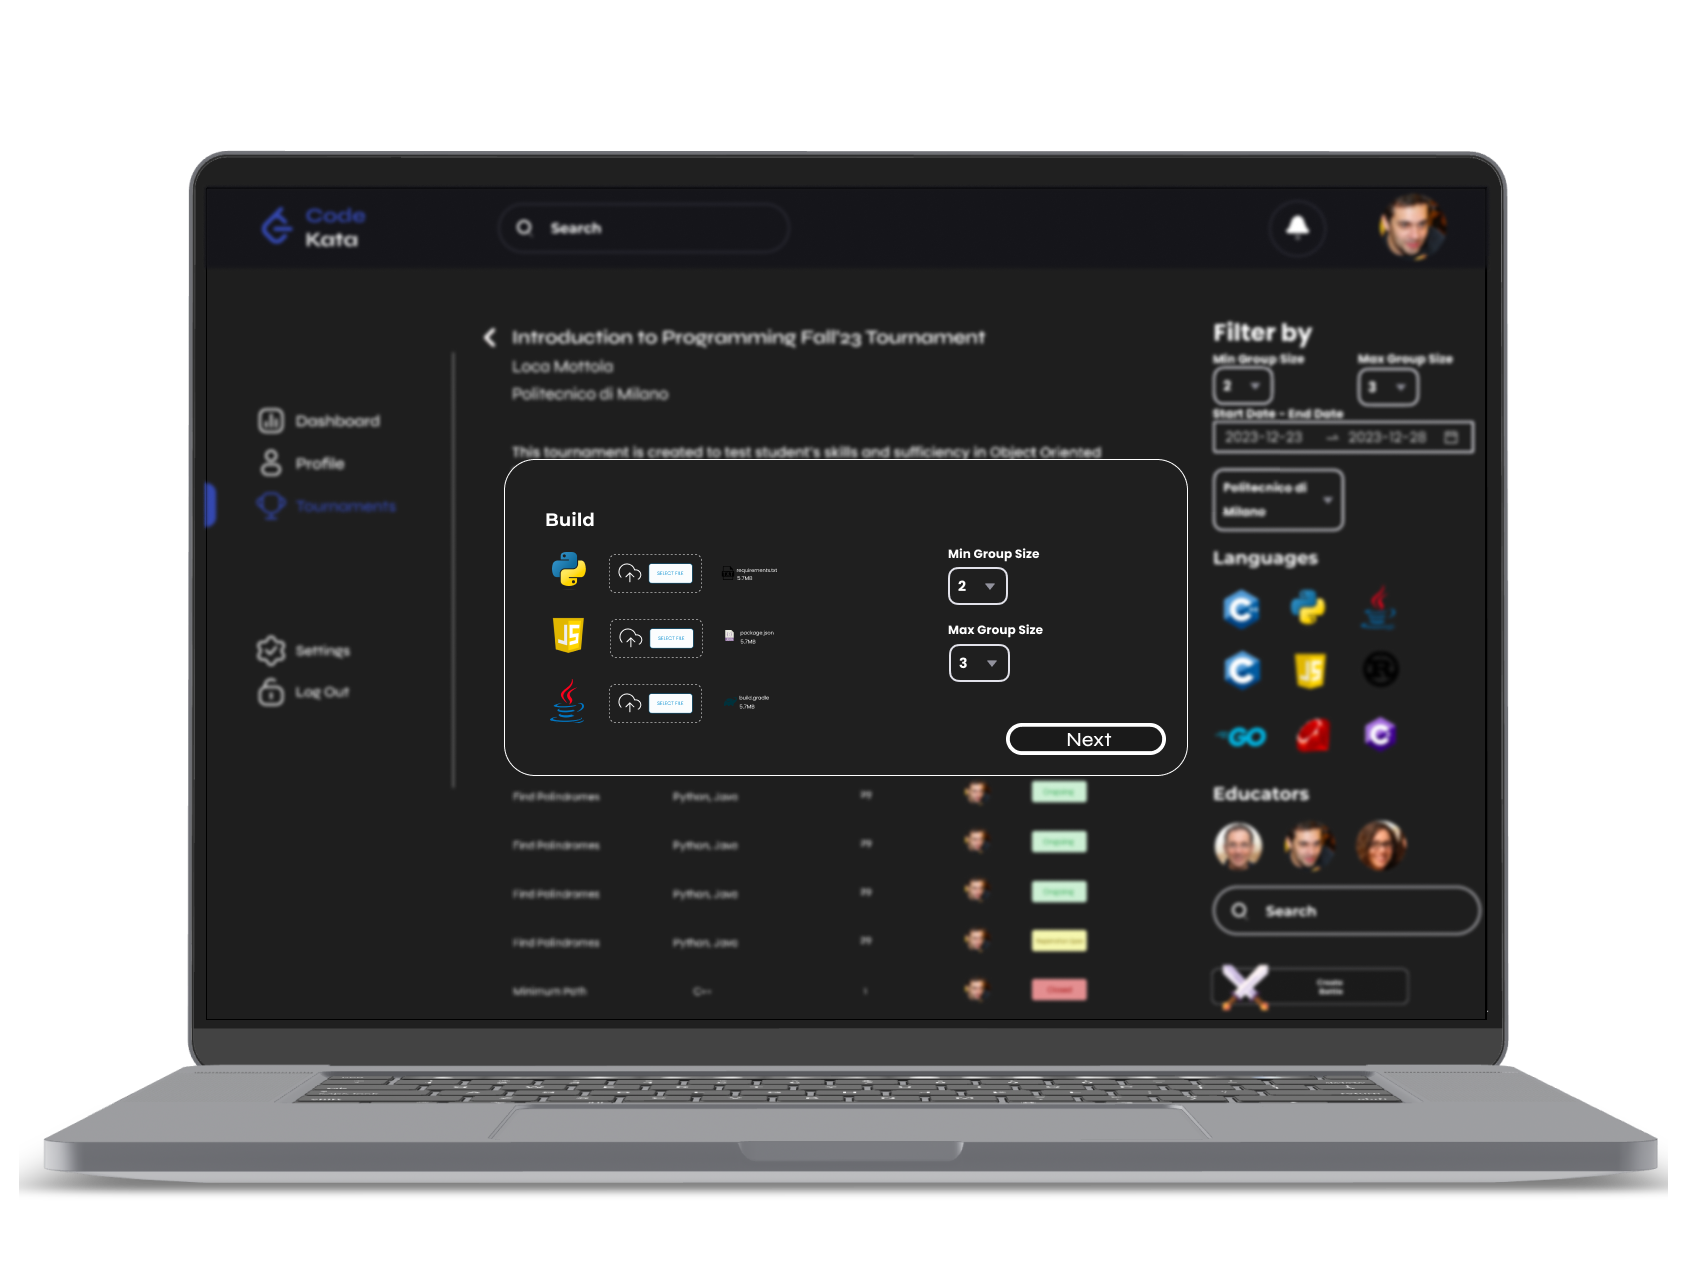
\includegraphics[scale=0.13]{Images/ui-ux/educator_creates_battle_5.png}
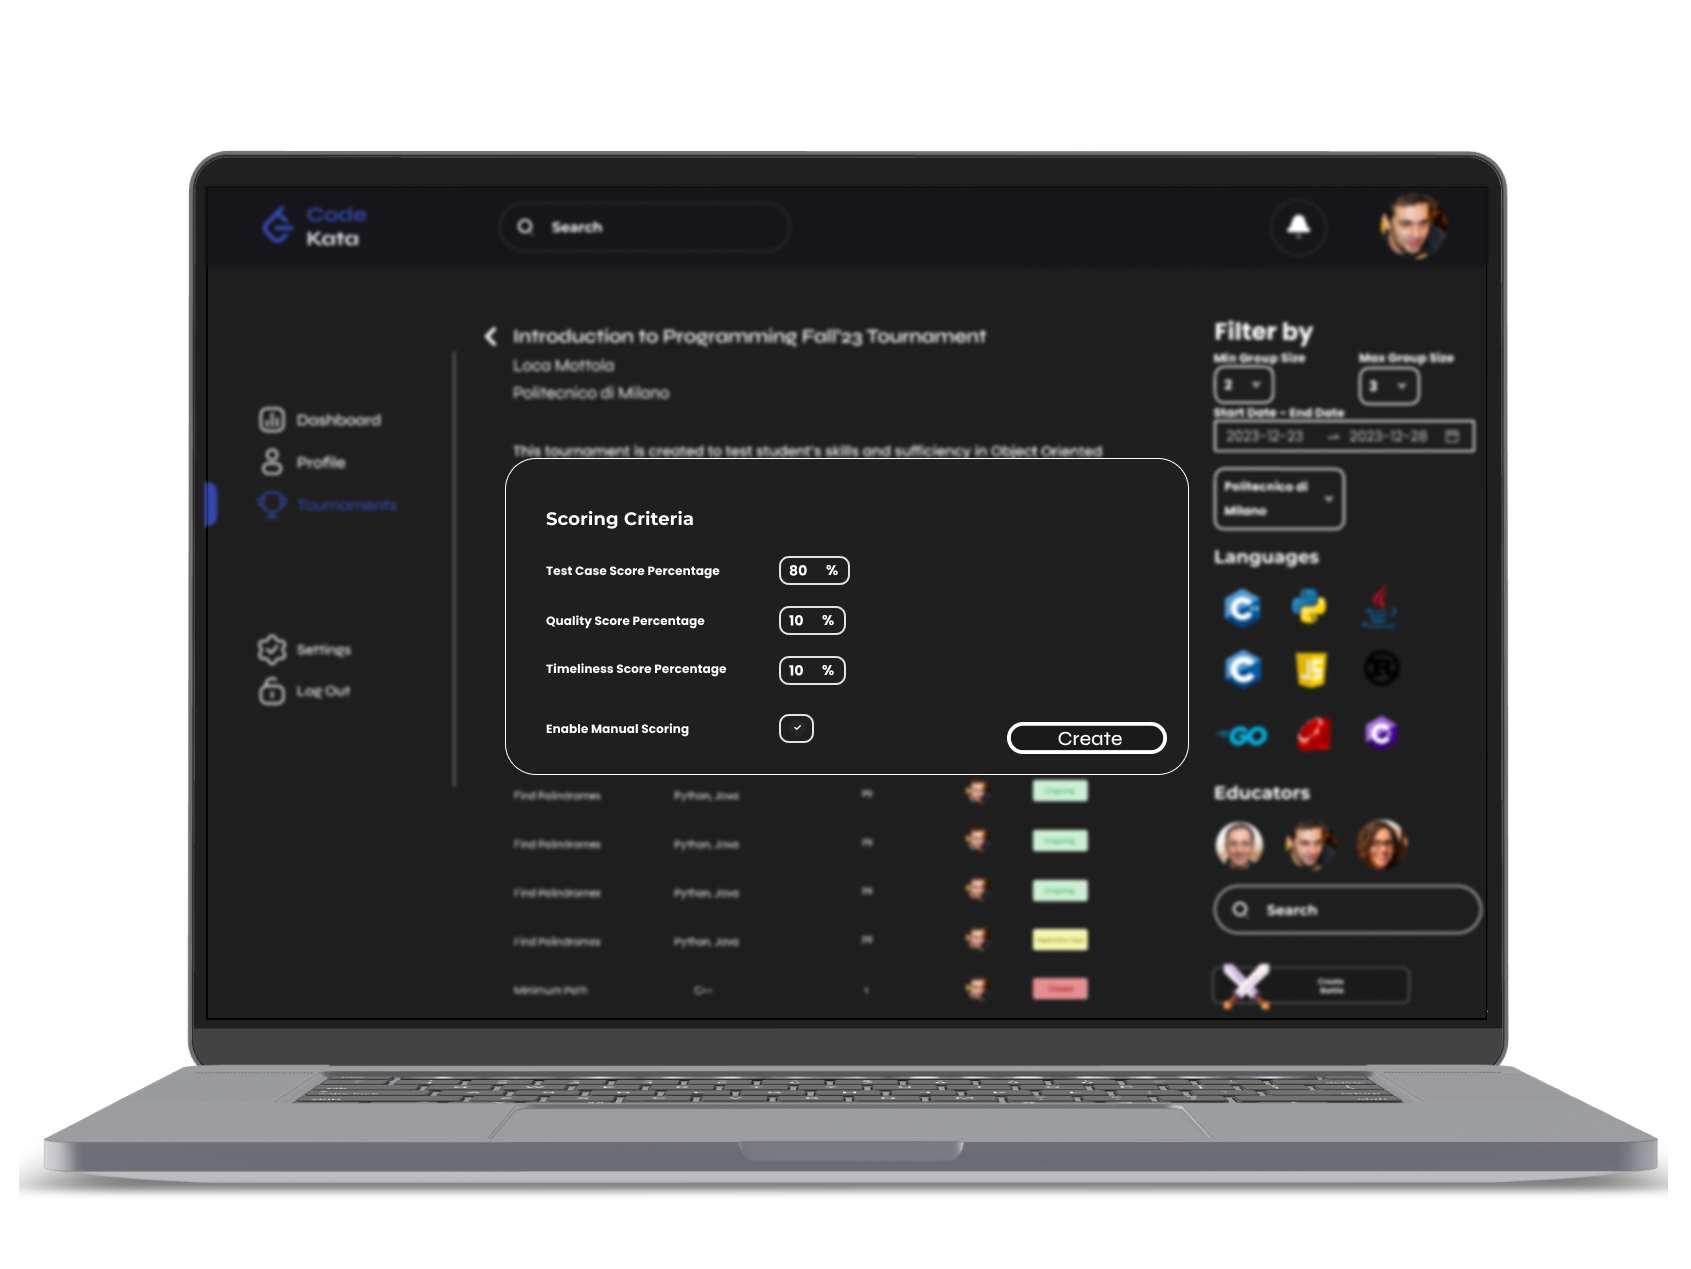
\includegraphics[scale=0.13]{Images/ui-ux/educator_creates_battle_6.png}
        (l) $UI_{12}$ Educator Creates Battle
\end{center}
\newpage
\begin{center}
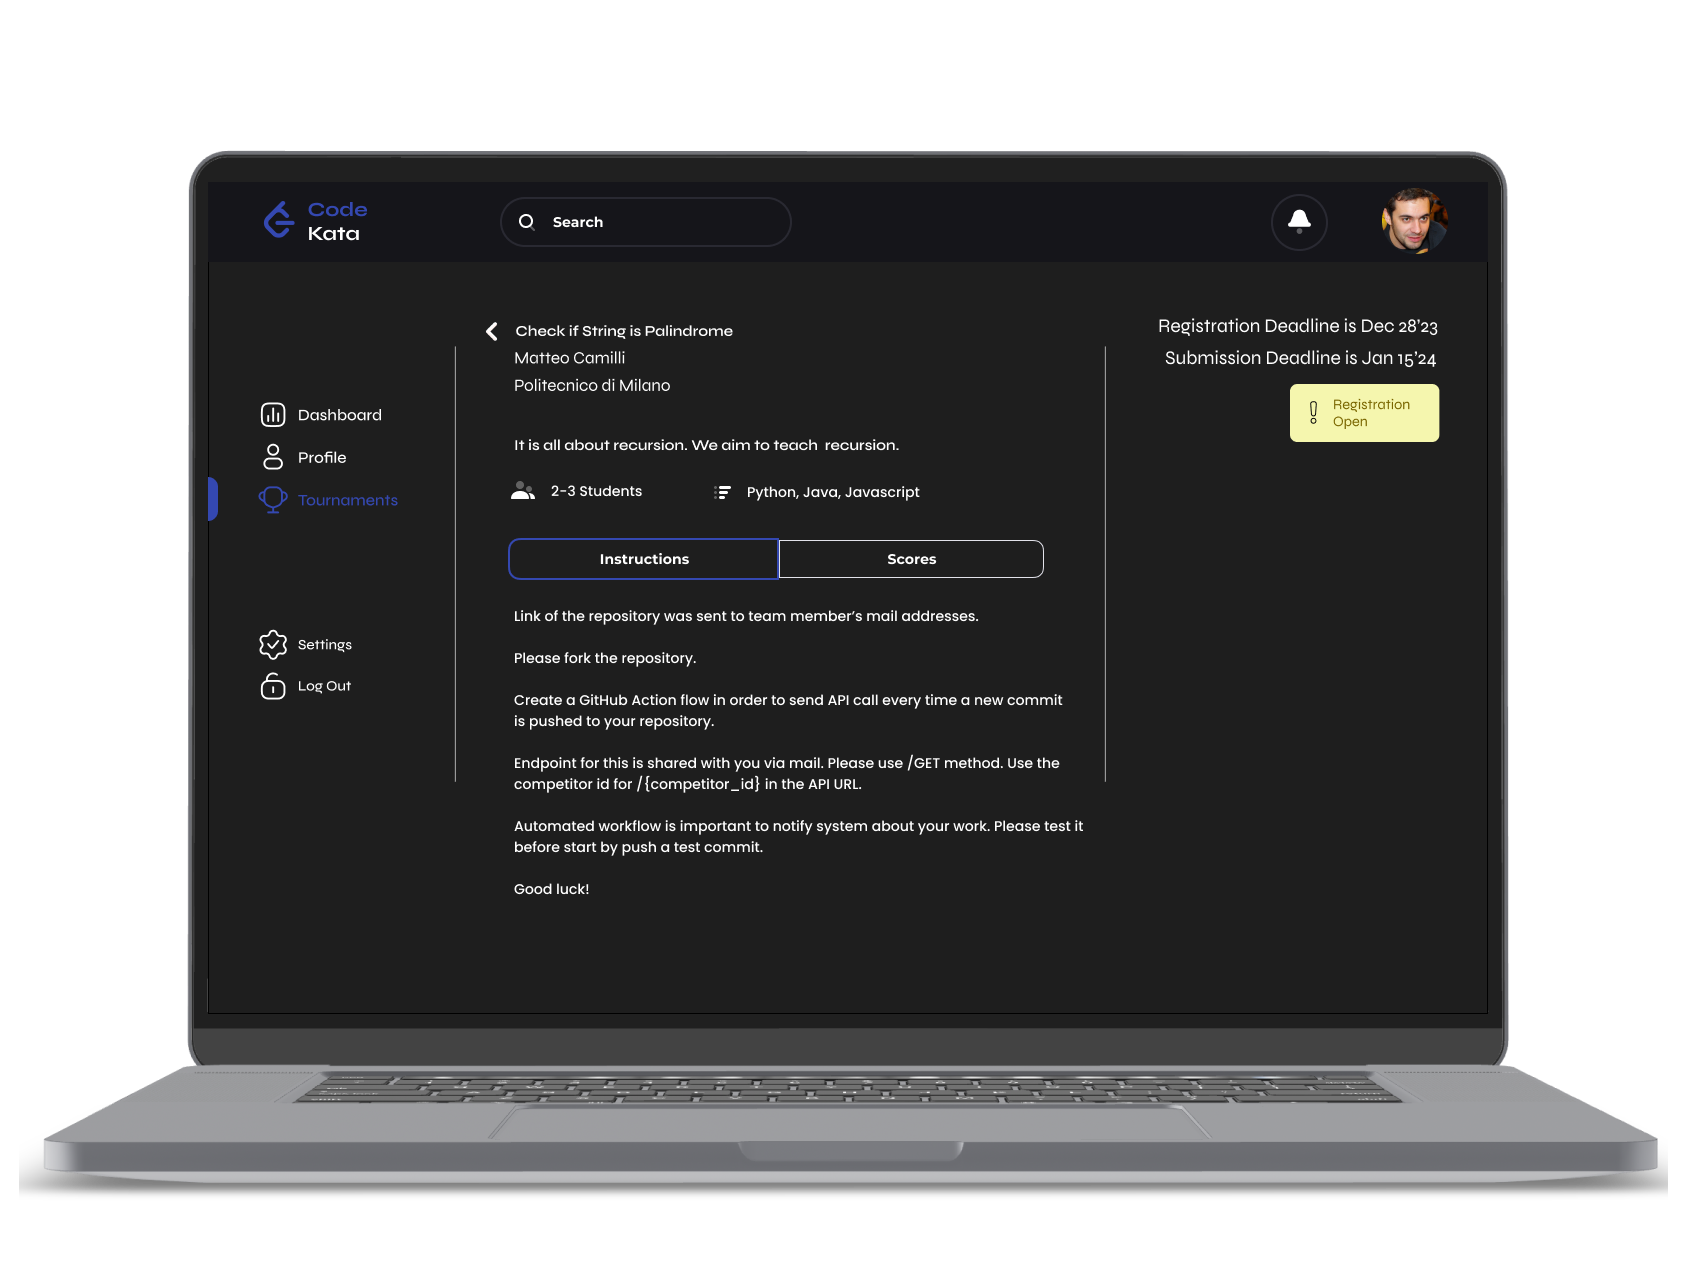
\includegraphics[scale=0.13]{Images/ui-ux/educator_battle_1.png}
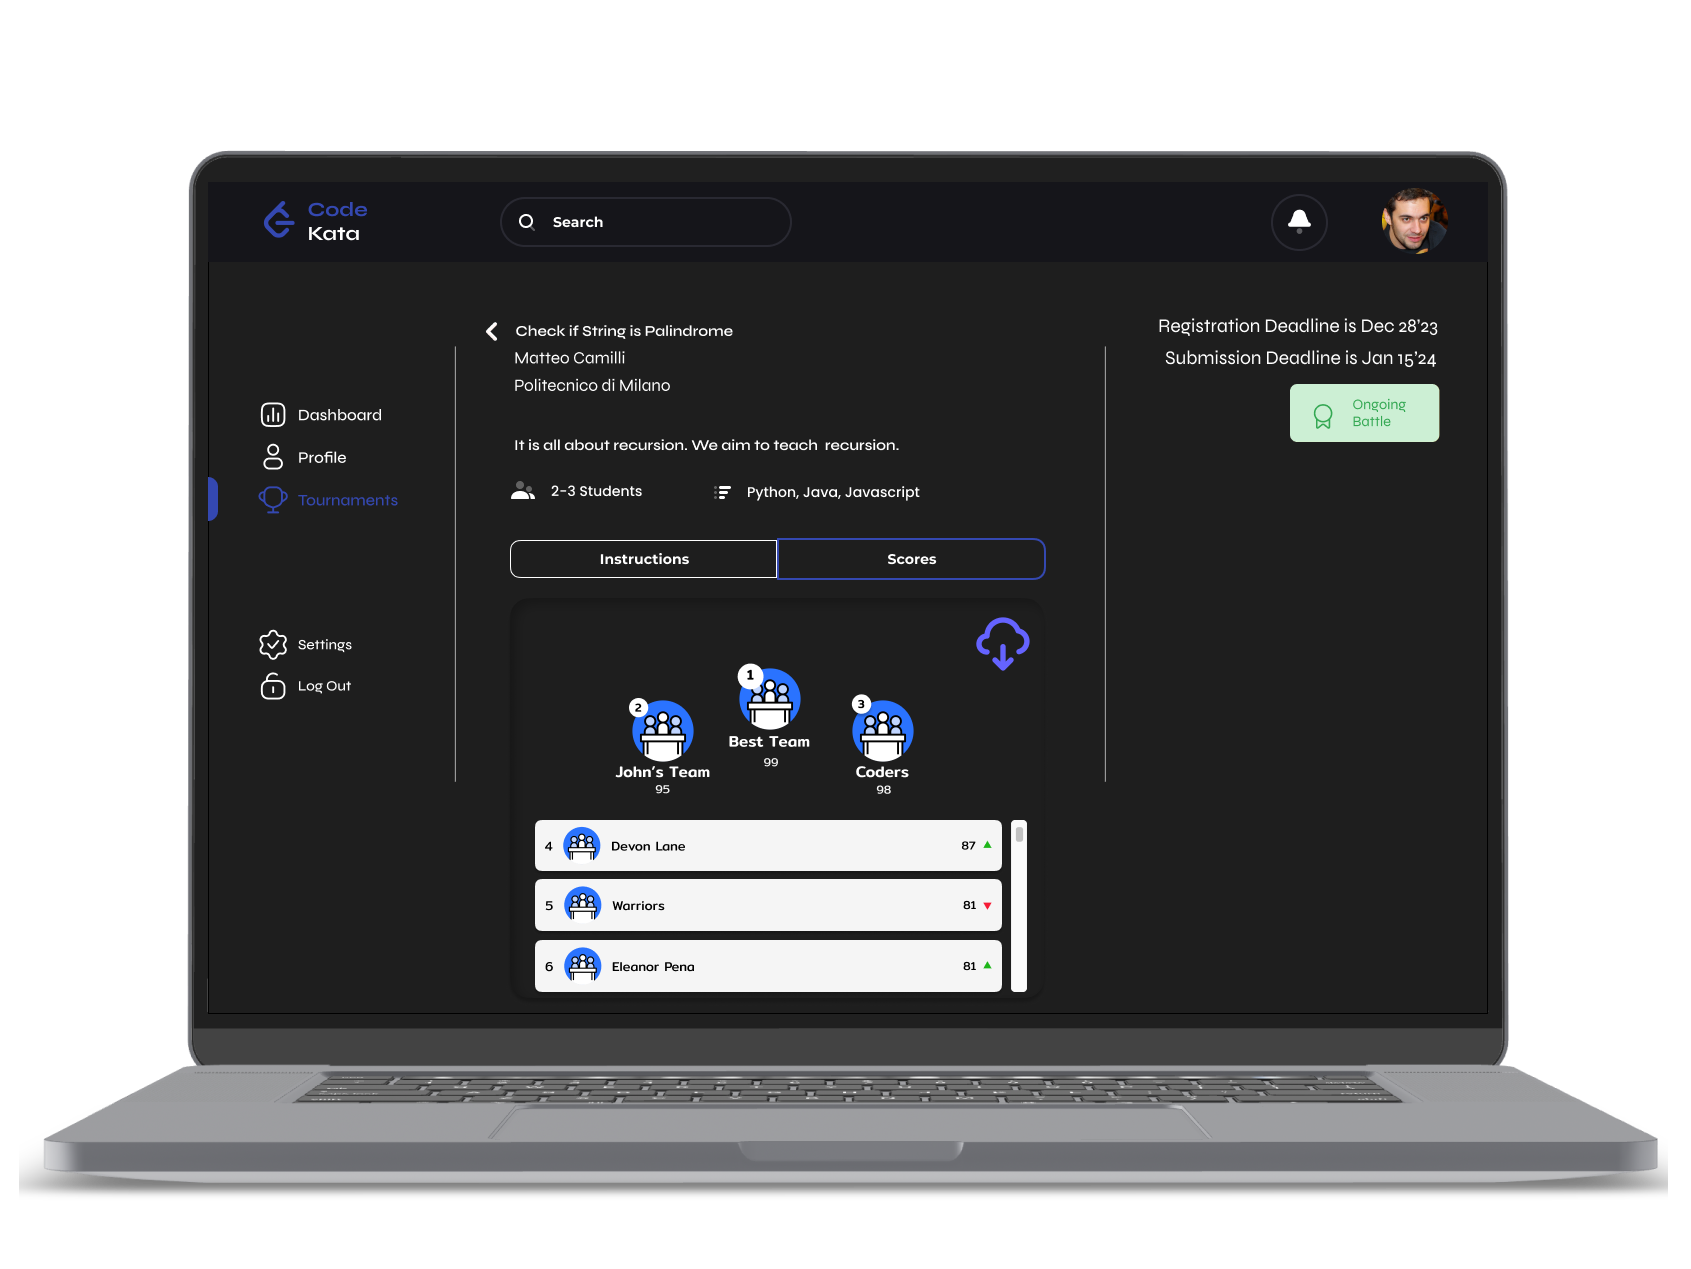
\includegraphics[scale=0.13]{Images/ui-ux/educator_battle_2.png}
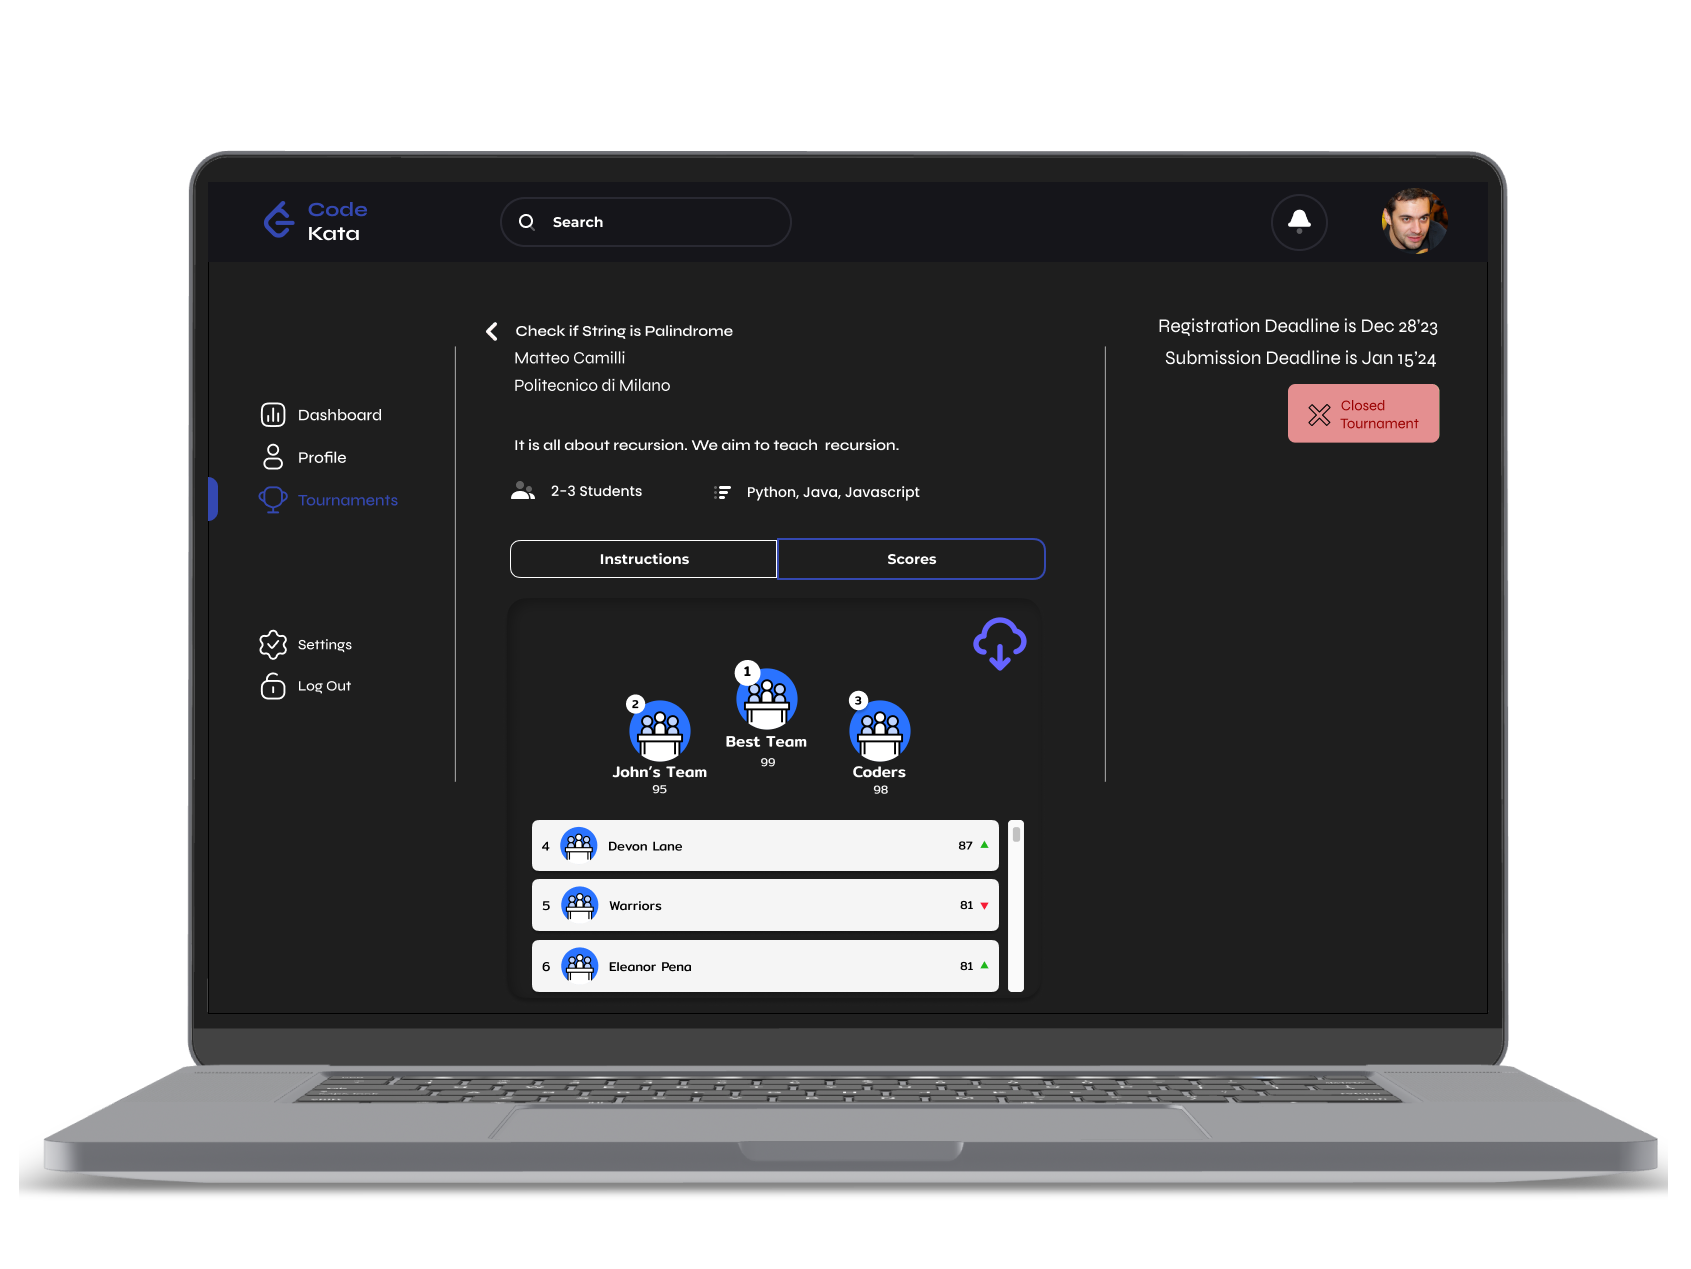
\includegraphics[scale=0.13]{Images/ui-ux/educator_battle_3.png}
\\ (m) $UI_{13}$  Educator visits Battle
\end{center}
\newpage
\begin{center}
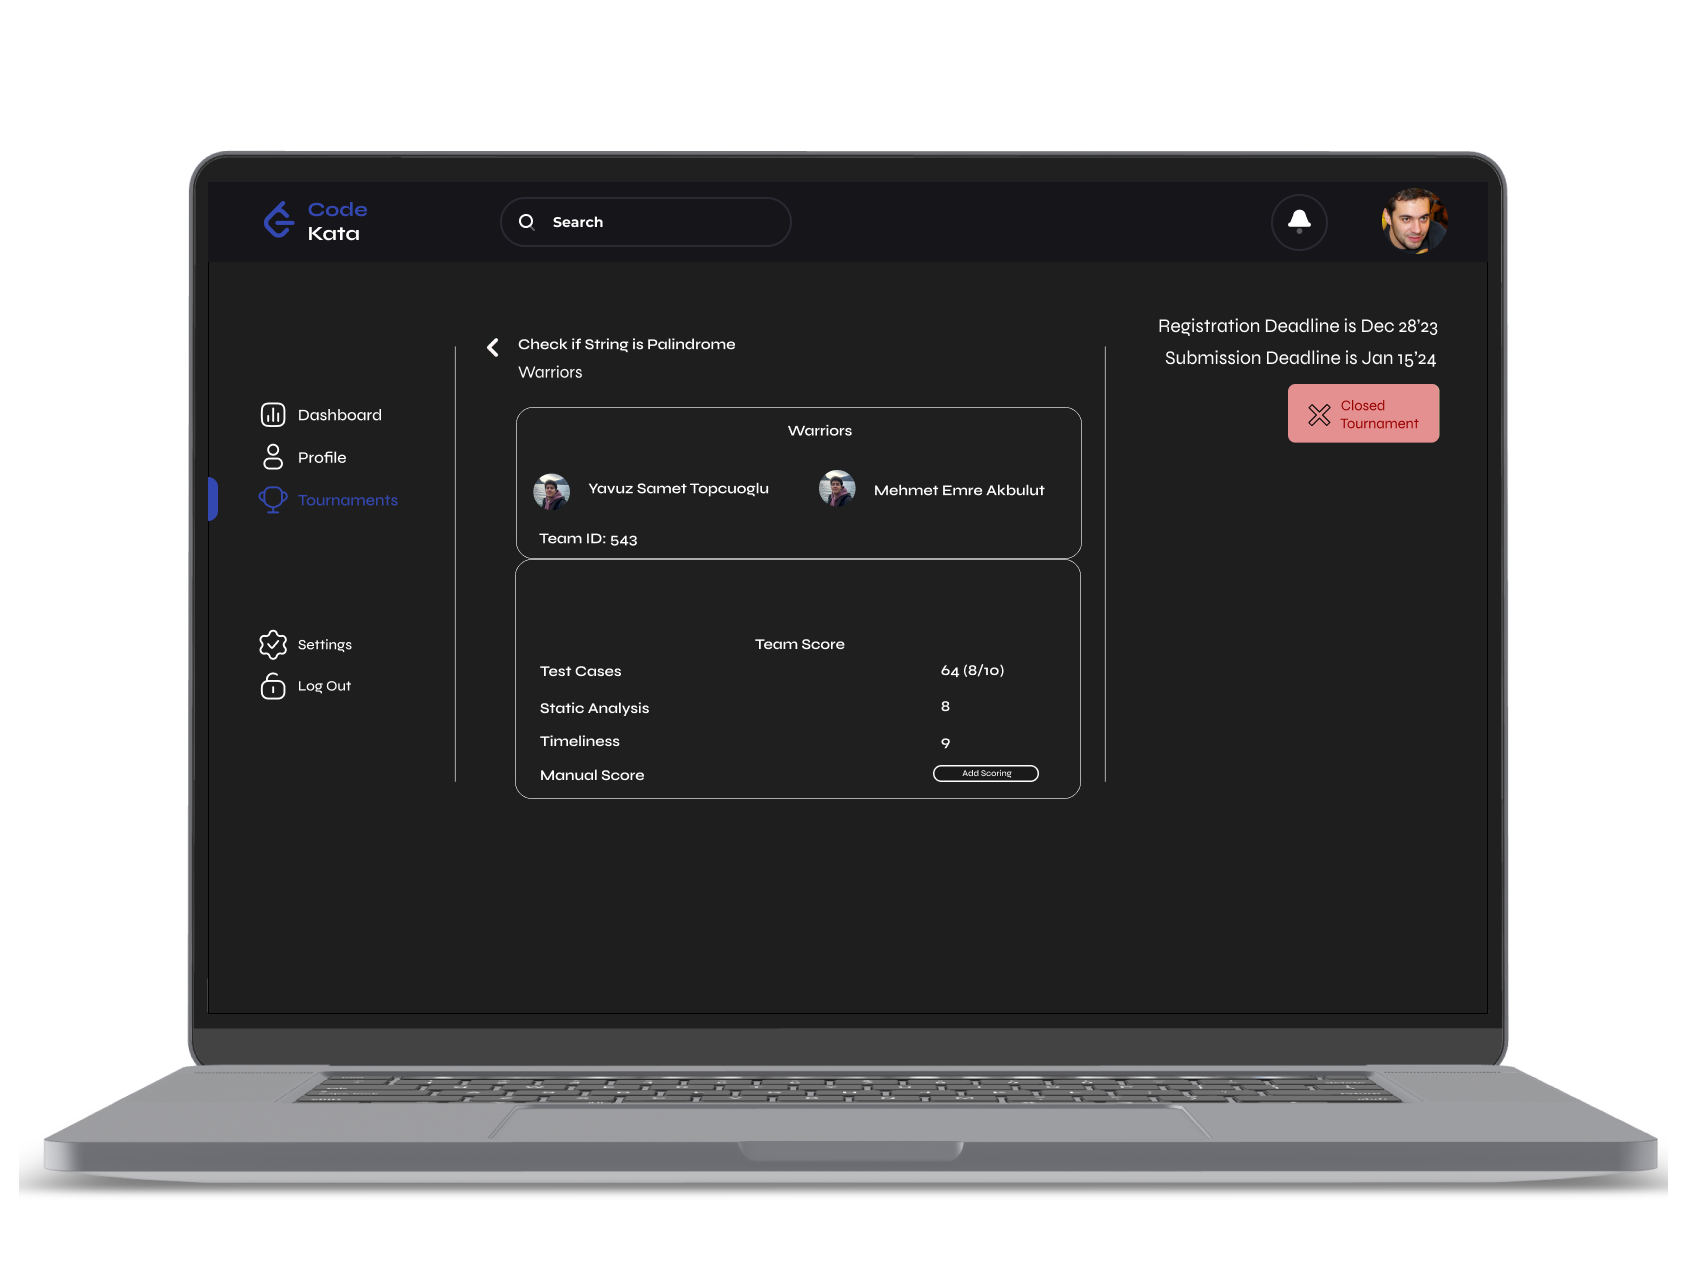
\includegraphics[scale=0.13]{Images/ui-ux/educator_team_1 (1).png}
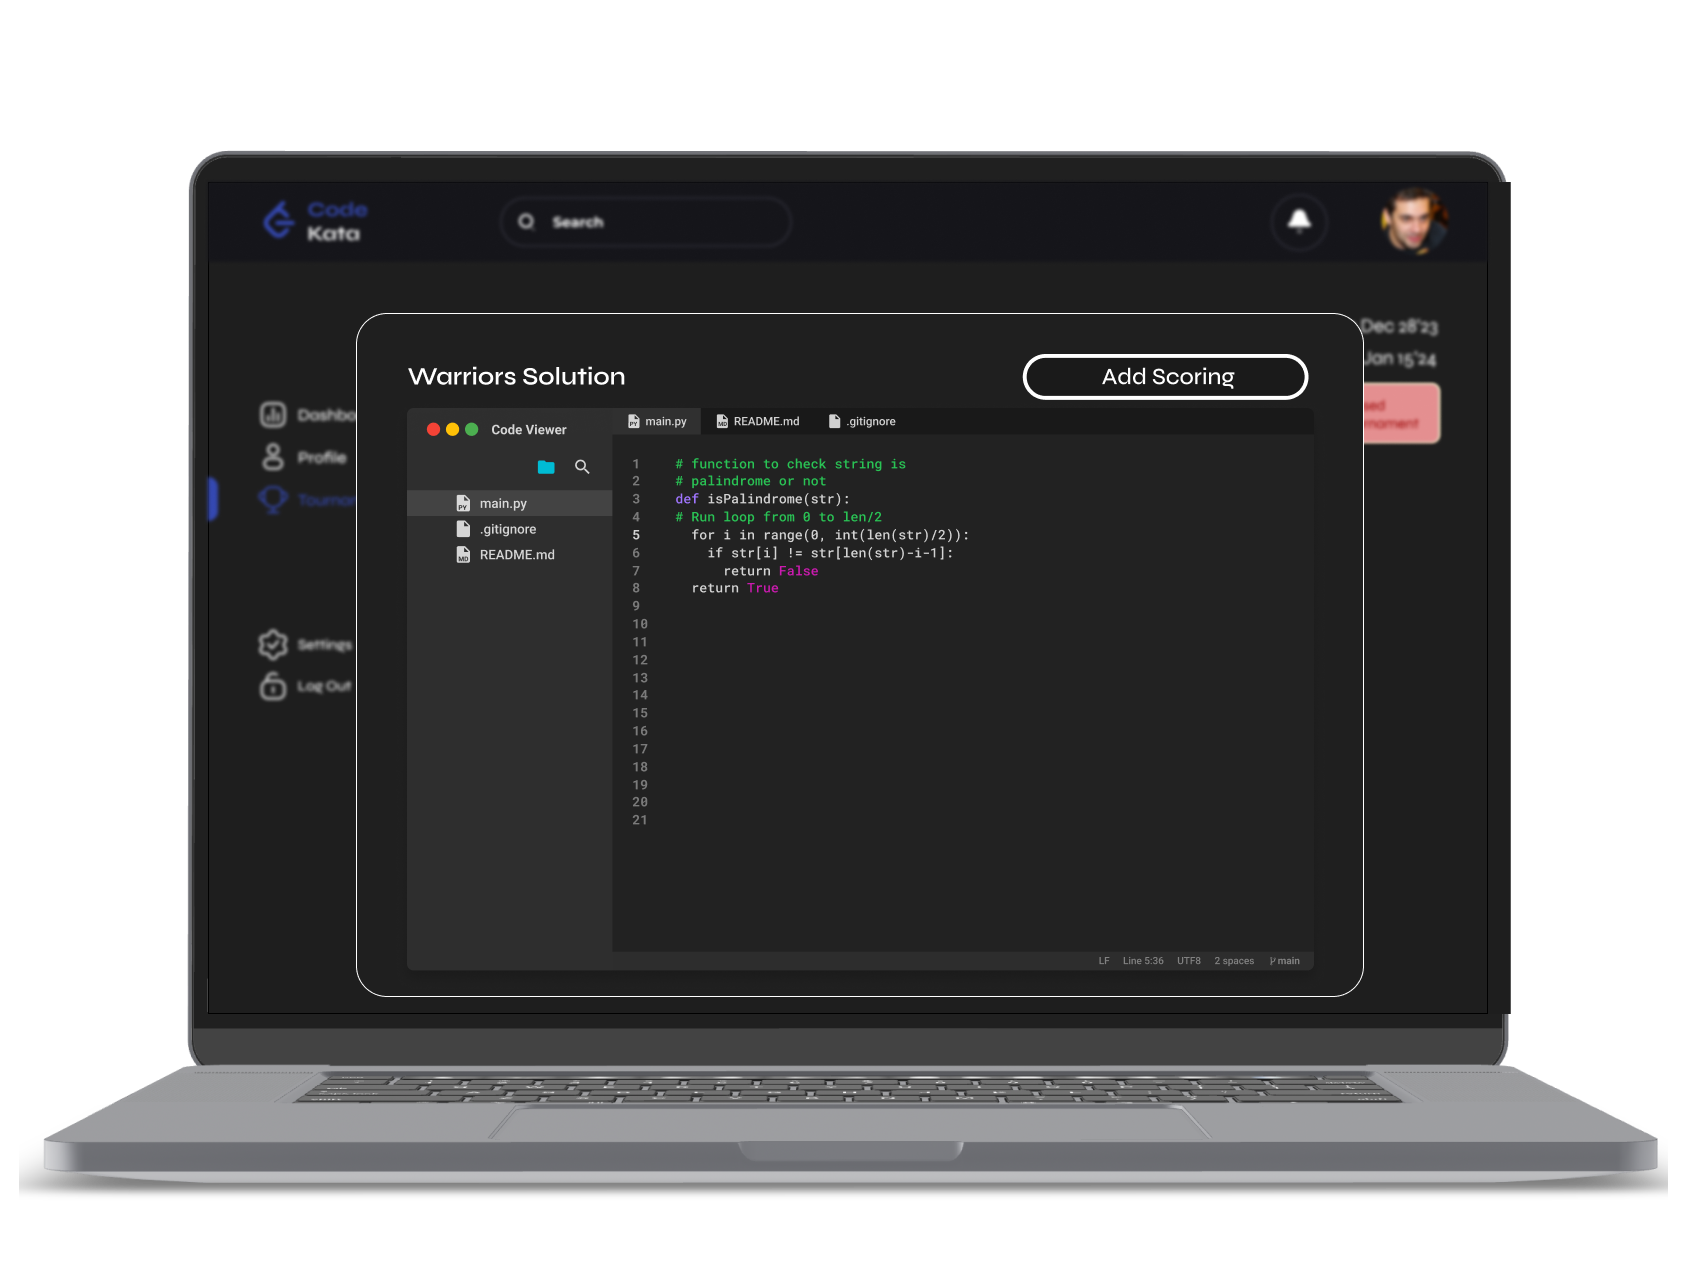
\includegraphics[scale=0.13]{Images/ui-ux/educator_team_2 (1).png}
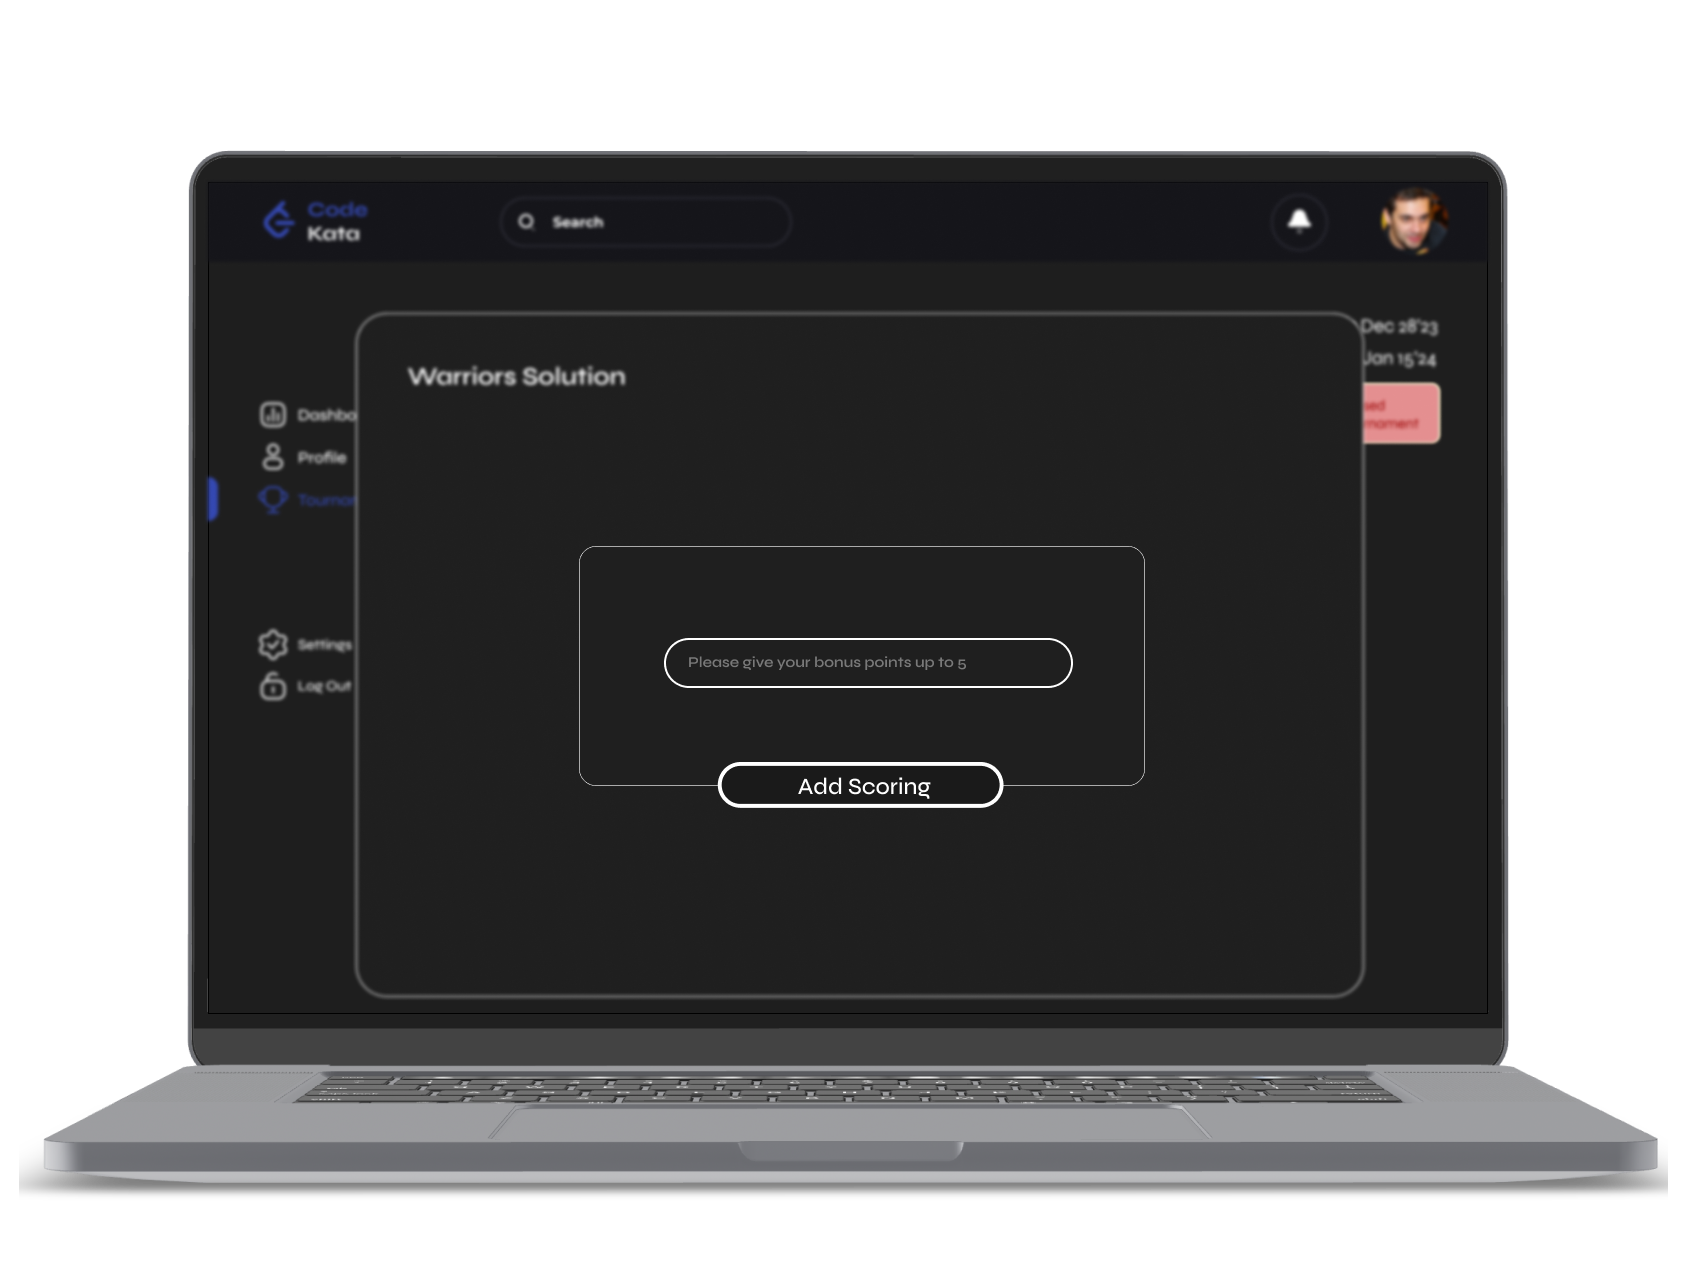
\includegraphics[scale=0.13]{Images/ui-ux/educator_team_3 (1).png}
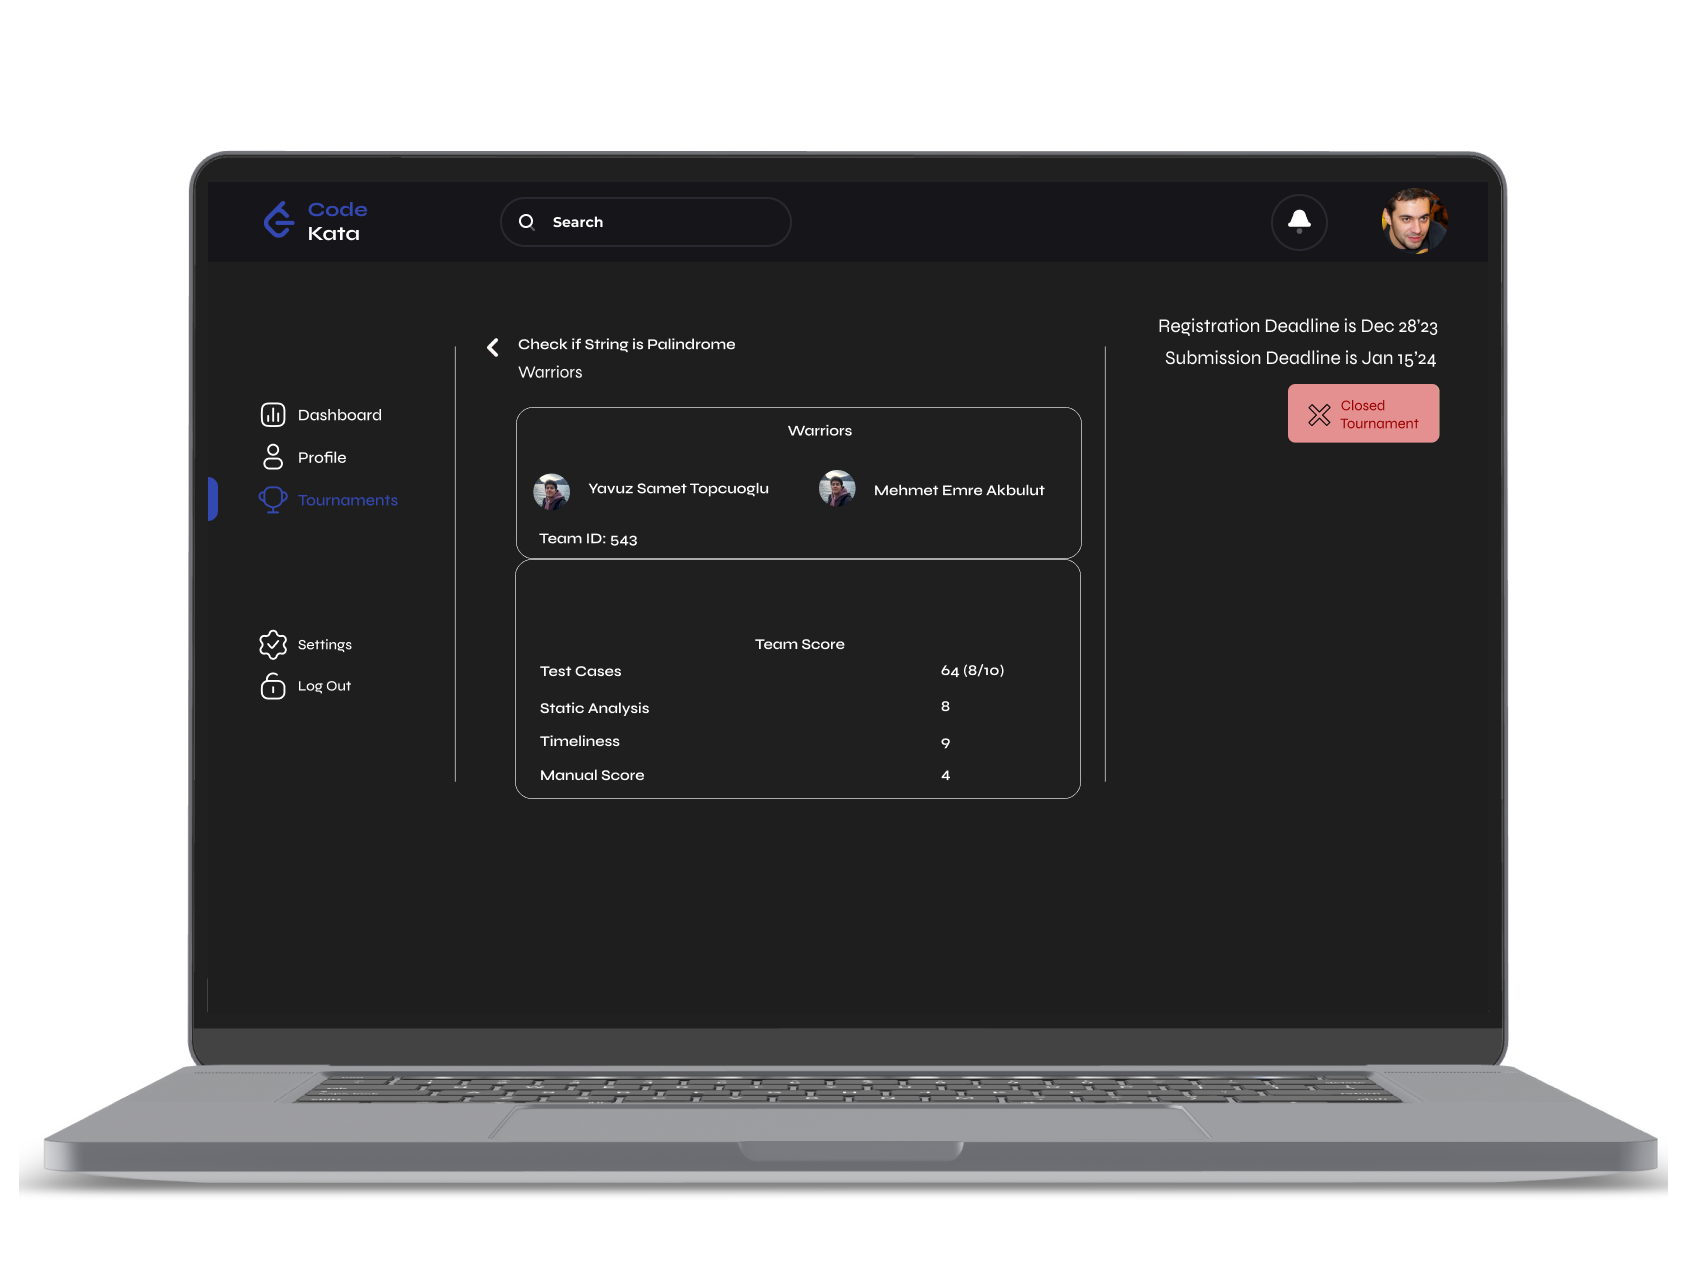
\includegraphics[scale=0.13]{Images/ui-ux/educator_team_4 (1).png}
        (n) $UI_{14}$  Educator, Team and Manual Scoring
\end{center}
\begin{center}
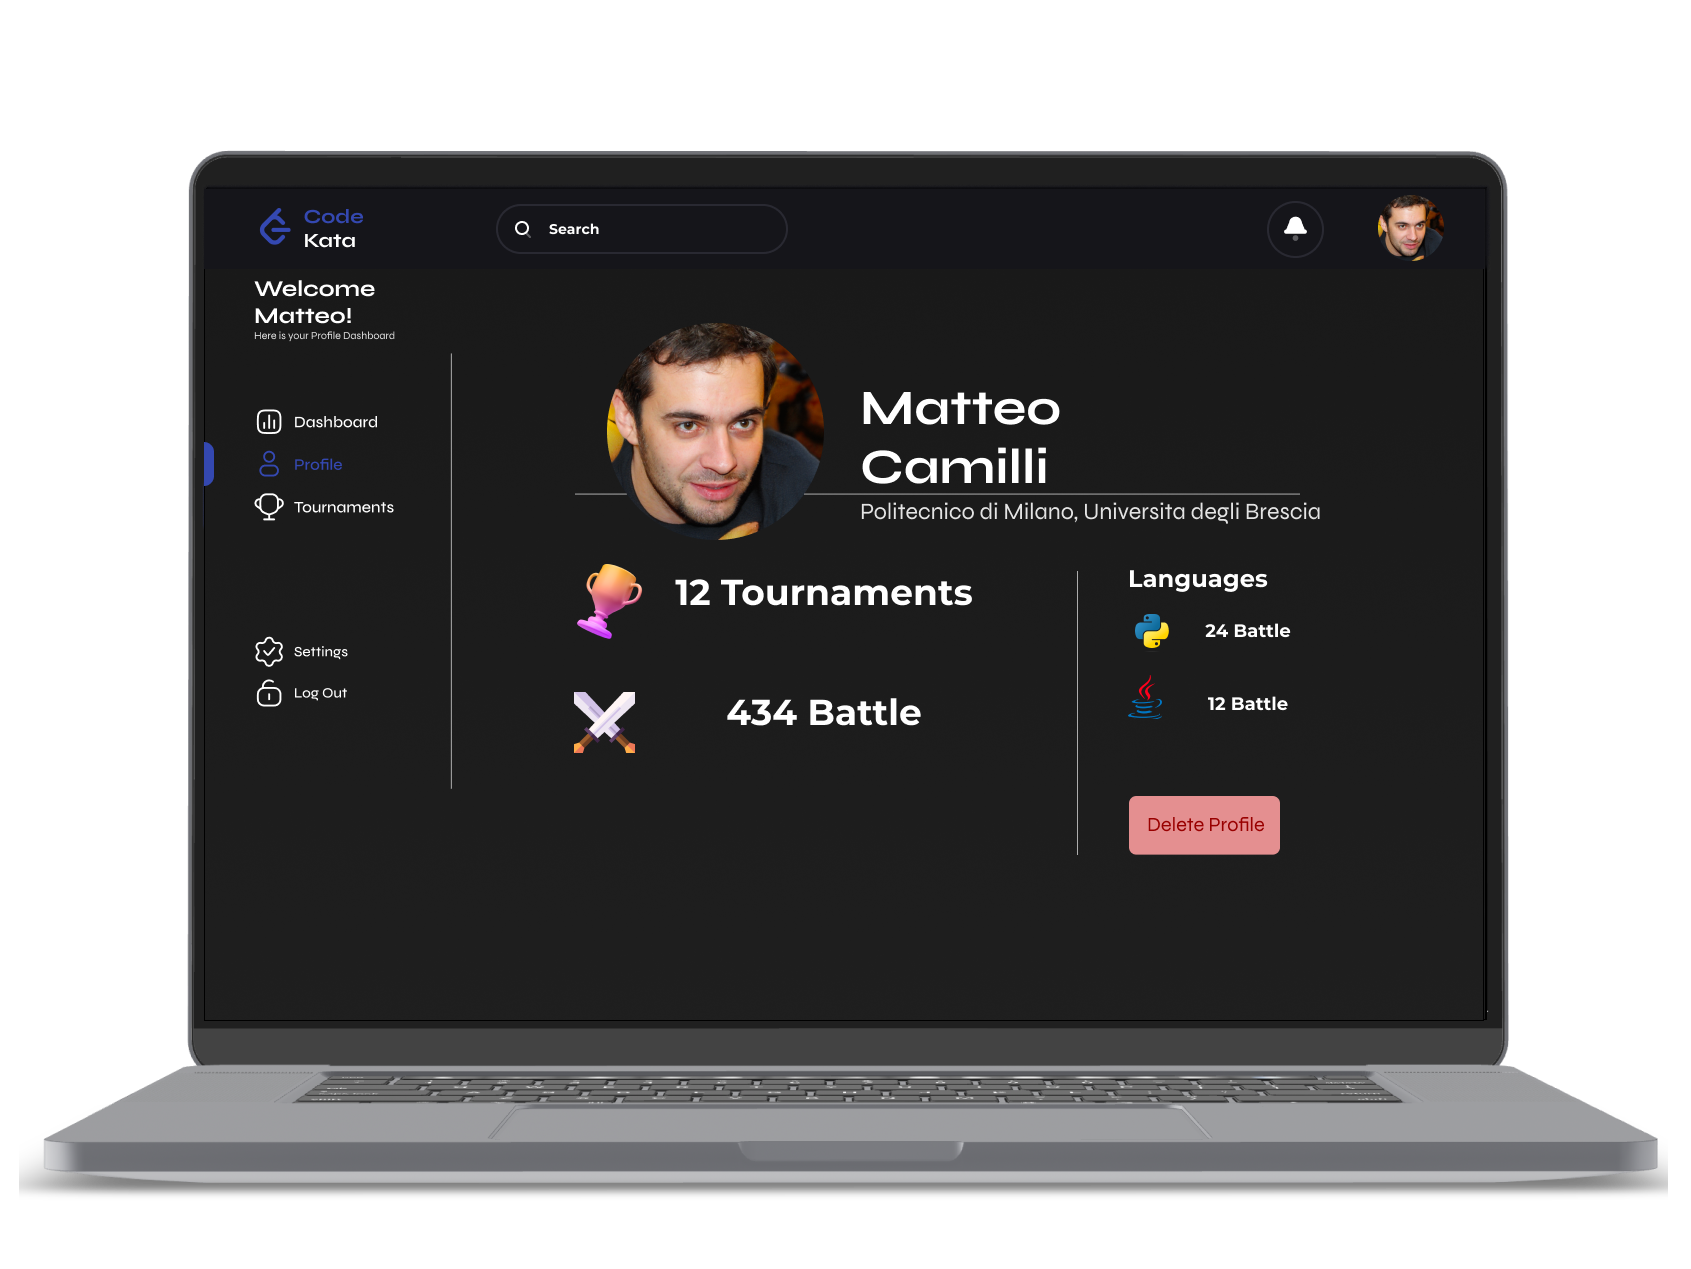
\includegraphics[scale=0.13]{Images/ui-ux/educator_profile.png}
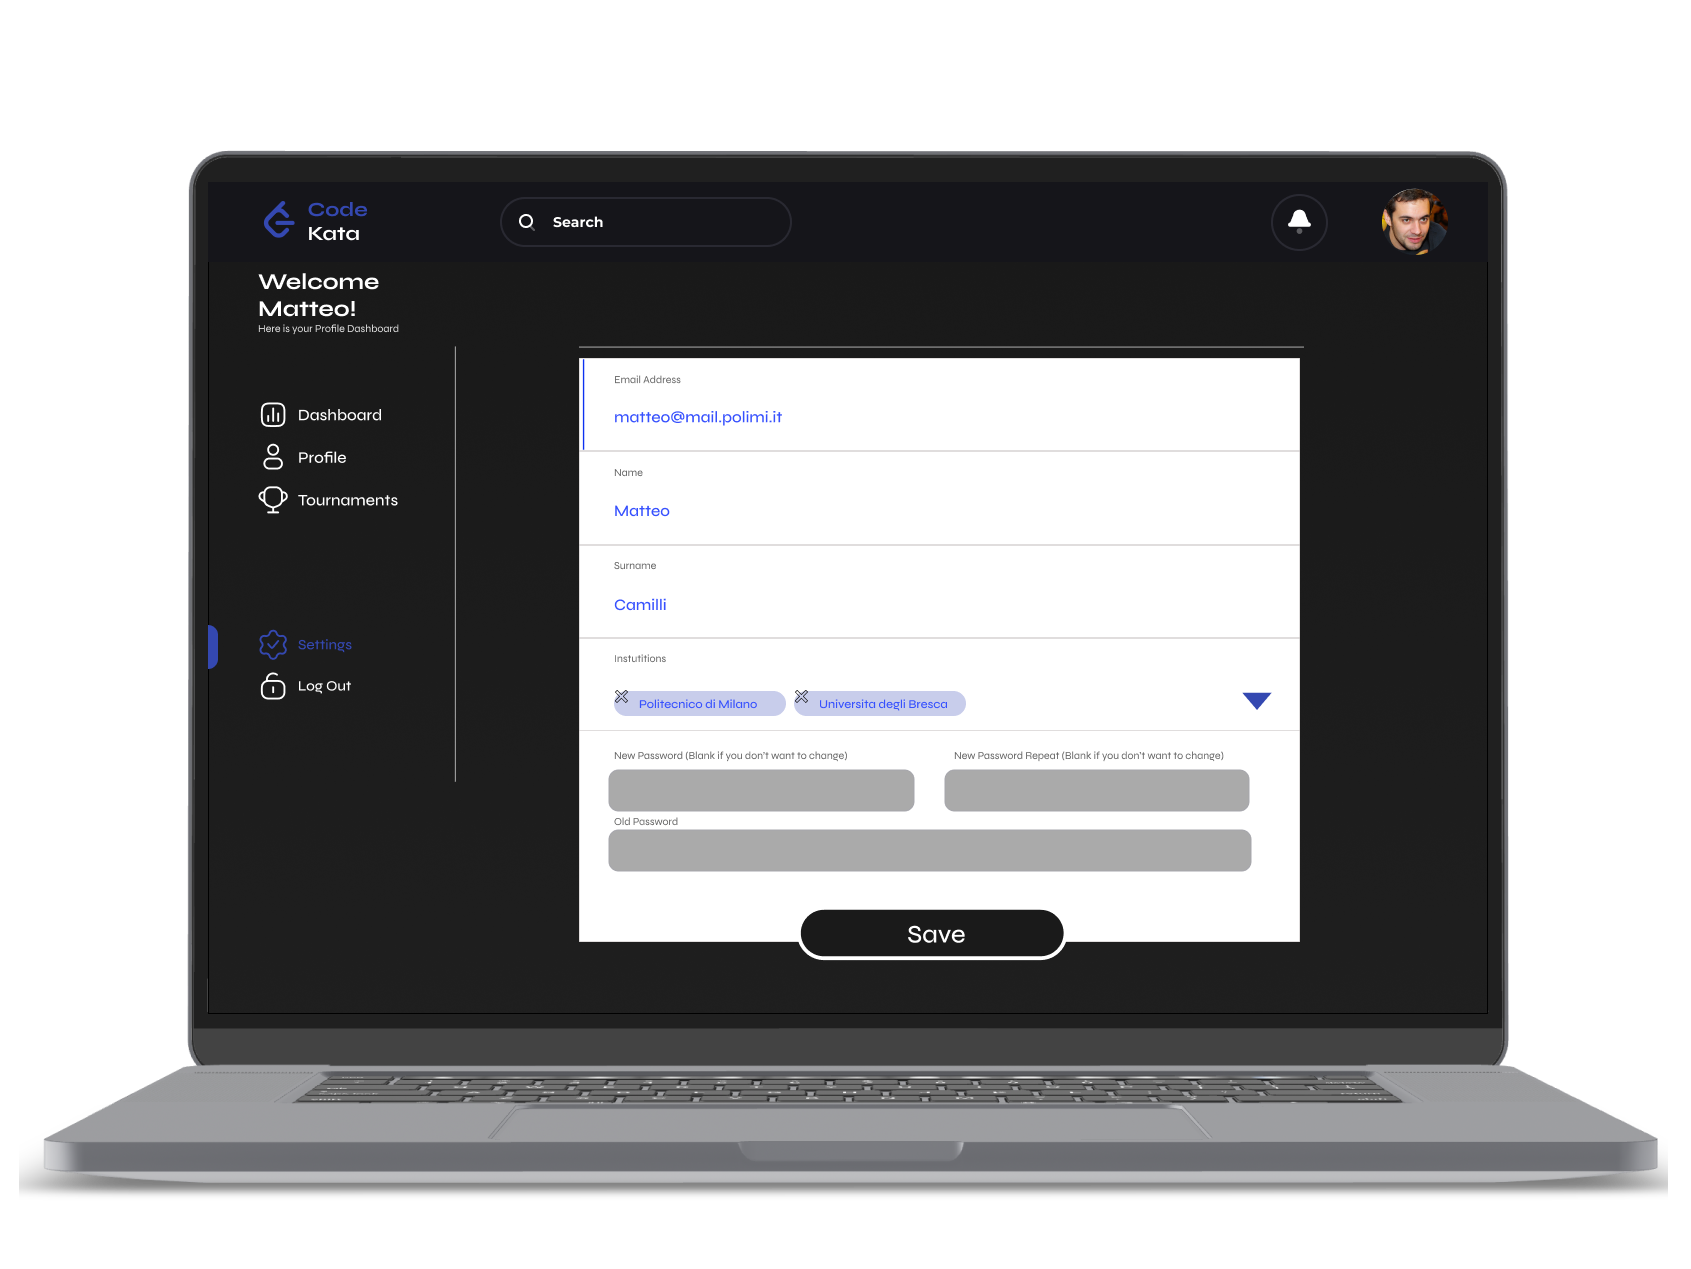
\includegraphics[scale=0.13]{Images/ui-ux/educator_settings.png}
        (o) $UI_{15}$  Educator Profile and Settings
\end{center}
\newpage
\begin{center}
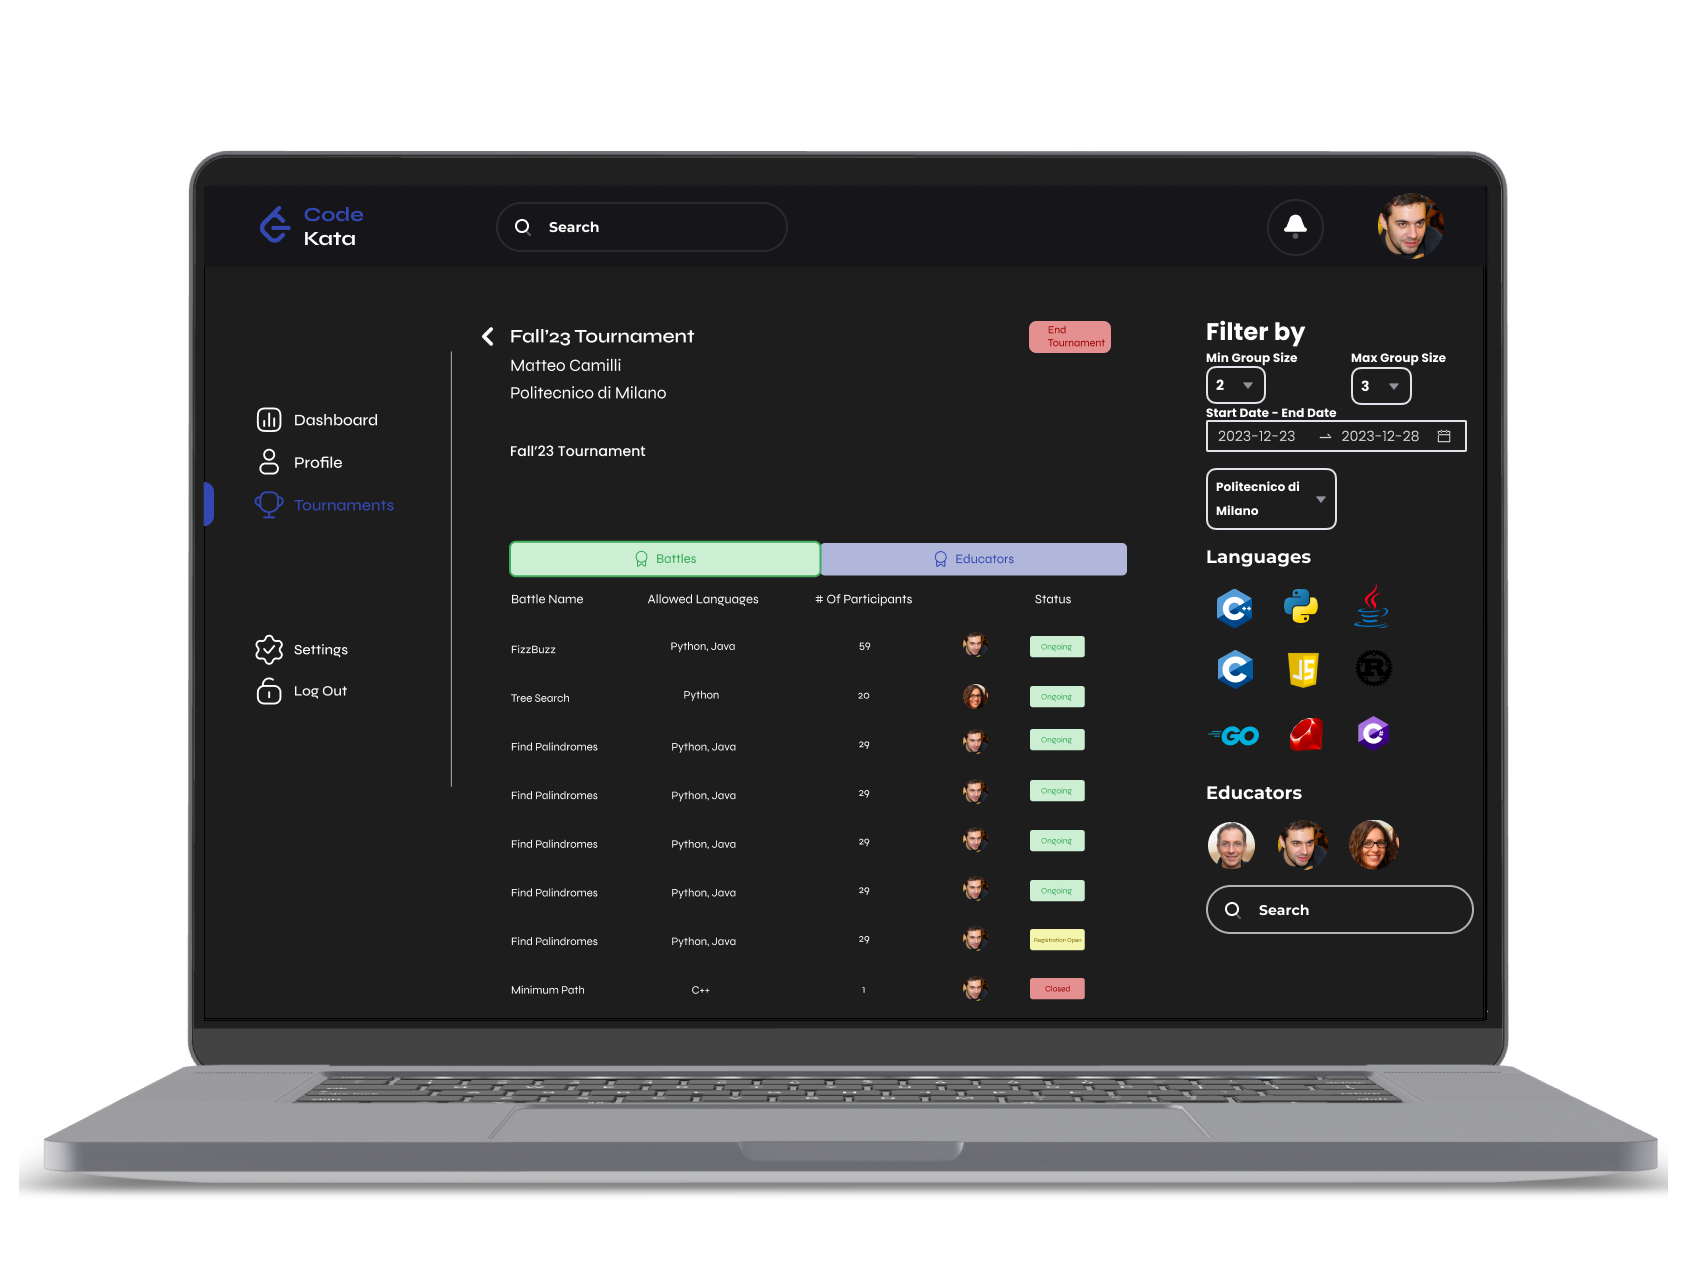
\includegraphics[scale=0.13]{Images/ui-ux/educator_end_tournament.png}
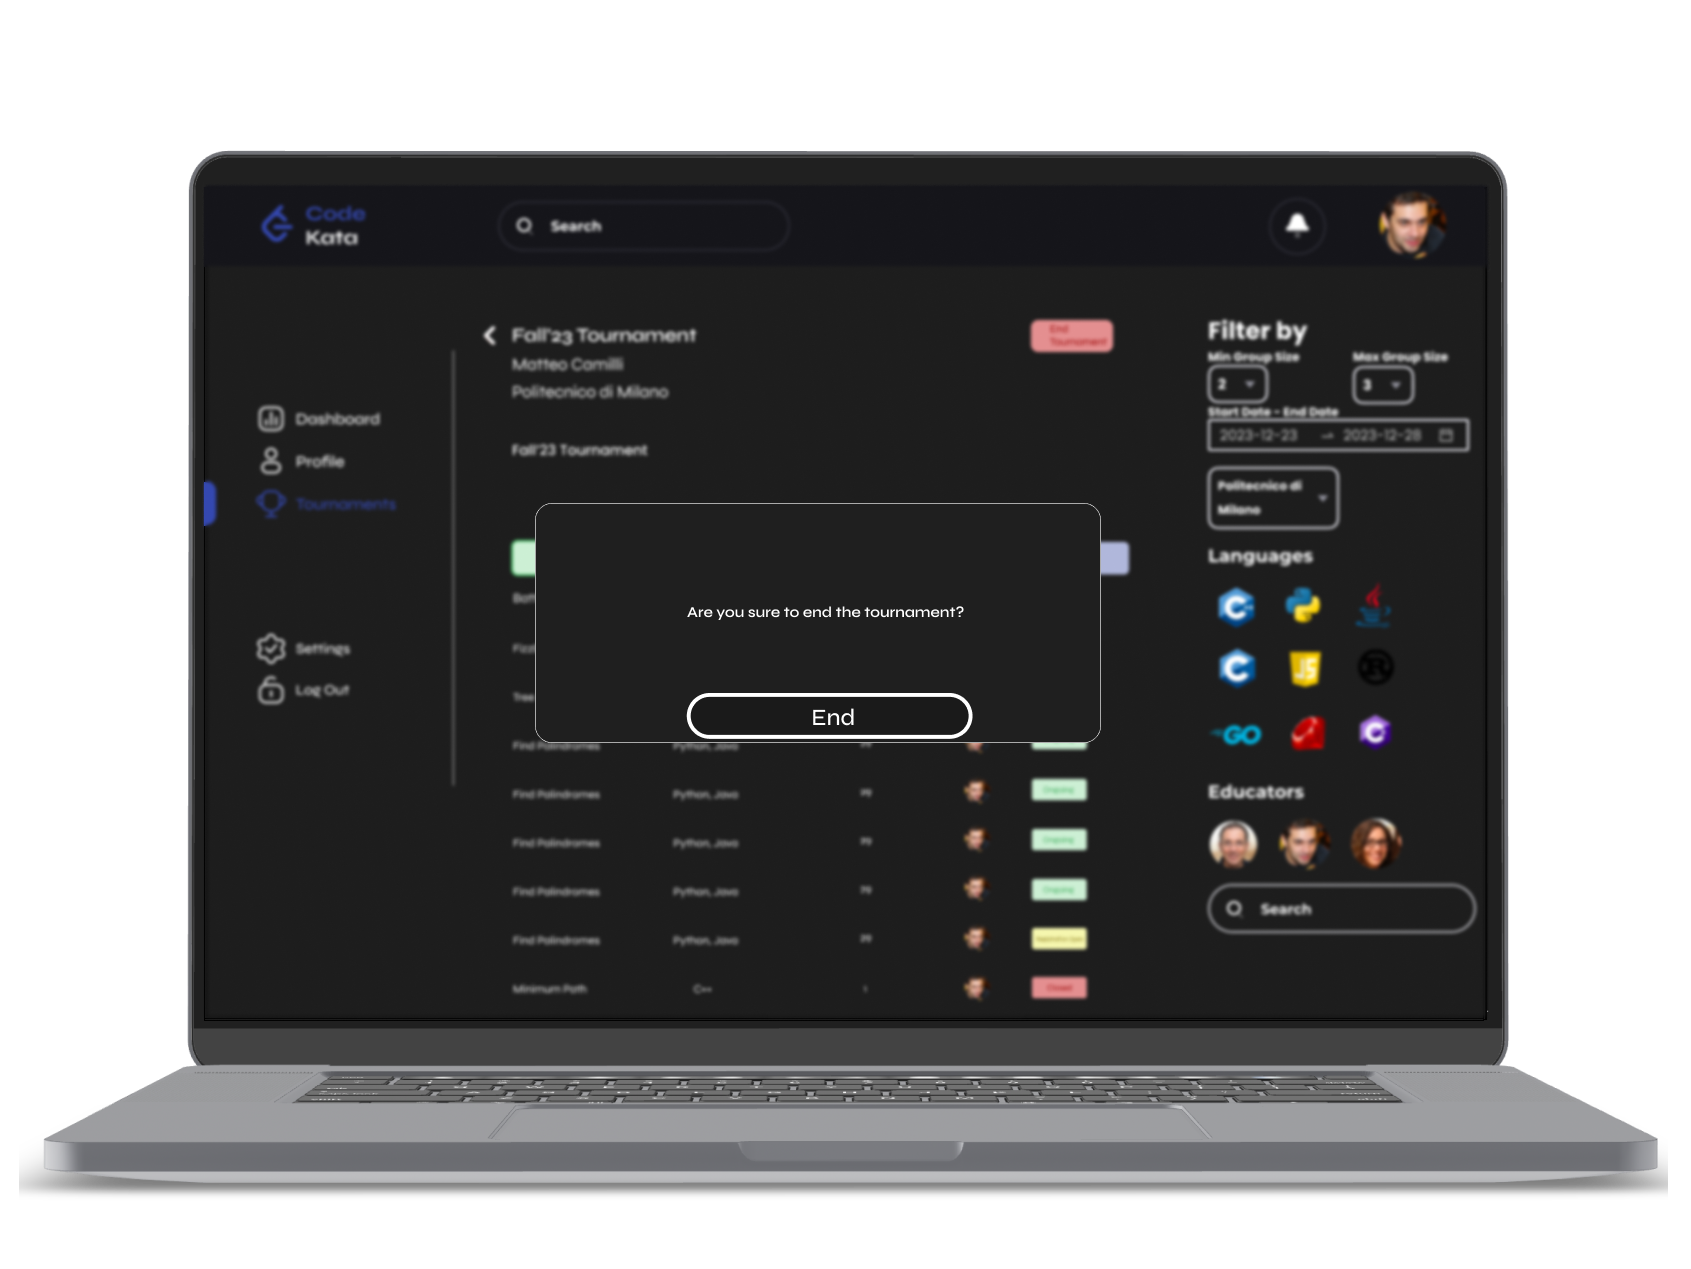
\includegraphics[scale=0.13]{Images/ui-ux/educator_end_tournament_1.png}
        (p) $UI_{16}$  Educator Ends Tournament
\end{center}

\begin{itemize}
    \item \textbf{$UI_{1}$:} This is a mockup for registration of students and educators. $RW_{1}$ is the related runtime diagram for this mockup.
    \item \textbf{$UI_{2}$:} This is mockup for student and educator login. $RW_{2}$ is the related runtime diagram for this mockup.
    \item \textbf{$UI_{3}$:} These are the screens of the student when it enters the application. This screens is created by fetching tournament with different filters.
    \item \textbf{$UI_{4}$:} These are screens of tournaments from students' perspective. Also these screens are related to  $RW_{3}$. Student can easily navigate among different tournaments.
    \item \textbf{$UI_{5}$:} These are screens of a single tournament from users' perspective. Also these screens are related to  $RW_{3}$. User can easily navigate among battles and leaderboard.
    \item \textbf{$UI_{6}$:} In this screen student register for battle by choosing "register as team" option. The following user interfaces $UI_{7}$ also explain the next steps from this design. Related to $RW_{10}$
    \item \textbf{$UI_{7}$:} This screens shows possible states of a battle screen for a student. Also related to $RW_{4}$ and and $RW_{10}$.
    \item \textbf{$UI_{8}$:} Profile and Setting screens of a student. Related to $RW_{5}$
    \item \textbf{$UI_{9}$:} These are the screens of the educator when it enters the application. This screens is created by fetching tournament with different filters.
    \item \textbf{$UI_{10}$:} These are screens of tournaments from educators' perspective. Also these screens are related to  $RW_{3}$. Educators can easily navigate among different tournaments.
    \item \textbf{$UI_{11}$:} These screens demonstrate the pages for tournament creation. As you can see another educators can be invited. Related to $RW_{6}$ and $RW_{11}$
    \item \textbf{$UI_{12}$:} These screens demonstrate the pages for battle creation. Related to $RW_{6}$ and $RW_{12}$
    \item \textbf{$UI_{13}$:} These screens demonstrate the pages for viewing a battle.  Related to $RW_{4}$
    \item \textbf{$UI_{14}$:} These screen shows how educators can see a submission made by students. Also it demonstrates the manual scoring.
    Related to $RW_{13}$, $RW_{14}$ and $RW_{15}$
    \item \textbf{$UI_{15}$:} Profile and Setting screens of a educator. Related to $RW_{5}$
    \item \textbf{$UI_{16}$:} Educator ends tournament.
\end{itemize}

\newpage
